%\documentclass[]{../../../tex/classes/styledArticle}
%\usepackage{../../../tex/packages/hebrewSupport}
%\usepackage{../../../tex/packages/mathShortcuts}
%\usepackage{../../../tex/packages/theoremsSupport}

\documentclass[name=רשימות חדו''א 2א]{../../../tex/classes/noChapterMegasumPreamble}
\usetikzlibrary{calc}
\usepackage{../../../tex/packages/mathShortcuts}
\usepackage{../../../tex/packages/hebrewSupport}

\usepackage{pgfplots}
\usepackage{pstricks-add}

\newcommand\Is{\dequad \ }
\newcommand\hopen {[a, \wg)}
\newcommand\bto{\lim_{{b \to \wg^{-}}}}
\newcommand\lims{\ol{\lim}}
\newcommand\limii{\underline{\lim}}

\newcommand\cz {\mathrm{(C)\ }}
\newcommand\ab {\mathrm{(A)\ }}
\newcommand\embed{\hookrightarrow}

\newcommand\uni{\overset{u}{\to}}


 \author{שחר פרץ}
 \title{\name}
 \date{2026 סמסטר ב'}
\begin{document}
% 	\maketitle
	\renewcommand{\footrule}{\rule{\linewidth-19pt}{0.25pt}\vspace{-5pt}}
	\firstPage{2026B}
	\newpage
	
	\hfil \textit{תאריך קימפול: \today}

	\setcounter{section}{-1}	
\section[מבוא למבוא]{\en{Introduction to the Introduction}}
\subsection[רישיון]{License $\sim$ רישיון}
	\en{The following summary is provided under the GNU General Public License version 3 (GPLv3). It can be distributed and/or modified under the terms of the license, or any later version of it. Additional information can be found \href{https://www.gnu.org/licenses}{here}. }
	
	הסיכום להלן מסופק תחת רשיון התוכנה החופשית של גנו גרסה 3 (GNU General Public License (GPL) version 3). ניתן להעתיקו ו/או להפיצו תחת GPLv3 או גרסה מאוחרת יותר. מידע נוסף אפשר למצוא \href{https://www.gnu.org/licenses}{כאן}. 
	
\subsection{הרבה מילים שאפשר לדלג עליהן}
	הסיכום להלן מבוסס על הרצאותיה של פרופסור יעל קרשון, ונכתב בסמסטר ב' של שנת 2026 (תשפ''ו). בניגוד לסיכומים אחרים (לפחות בשלב הזה) לא ערבו מקורות נוספים. כן הוספתי משפטים, הערות ואיורים לאחר הקלדת ההרצאות לסיכום לזה, ומי שמעוניין בהרצאות המקוריות מוזמן לבקר בגיטהאב שלי בתיקייה lec. 
	
	הפרק האחרון של הקורס, מרחבים מטריים, סוכם באופן עצמאי ומופיע כפרק הראשון של הסיכום (הכרגע עדיין־בשלבי־עבודה) שלי לטופולוגיה. לכן סיכום זה כולל שני פרקים עיקריים: אינטגרלי רימן וטורי פורייה. 
	
	\hfill שחר פרץ, 17.7.2026
	
	
\subsection{סימונים}
	בסיכום הבא נניח את הסימונים הבאים: 
	\begin{itemize}
		\item \hfil $[n] \cod \N \cap [0, n]$
		\item \hfil $\subset \; \cod \; \subseteq$
		\item \hfil $\bigcup A \cod \bigcup_{X \in A}X$
	\end{itemize}
	
%\subsection{רשימת נושאים שהוספתי לסיכום נוסף על החומר של הקורס}
	
	
	
	\newpage
	\setcounter{tocdepth}{3} % show subsubsections
	\tableofcontents
	
	%	\listoftheorems
	
	\middleText{\textit{בתיאבון}}

\section[אינטגרלי רימן]{\en{Riemann Integrals}}
\subsection{מבוא לחלוקות: חישוב אורך עקומות}
	\defi{בהינתן $a, b \in \R$ וכן $a < b$, \textit{קטע סגור} יוגדר להיות $[a, b] := \{c \mid a \le c \le b\}$}
	\exe{בהינתן קטע סגור, ניתן לעבור עליו בקצב אחיד. רמז:
	\[ \{c \mid a \le c \le b\} = \{(1 - \lg)a + \lg b \mid 0 \le \lg \le 1\} \]}
	\defi{\textit{חֲלוּקָה} של קטע $[a, b]$ (באנגלית – partition) היא קבוצה של $n + 1$ נקודות $\Pi = \{x_0, x_1 \dots x_n\}$ כאשר $n \in \N$, כך ש־$a = x_0 < x_1 < \cdots < x_n = b$. }
	מכאן, שכמות הנקודות בחלוקה היא {סופית}.
	\defi{בהינתן חלוקה, \textit{תת־הקטע ה־$i$} של החלוקה הוא $[x_{i - 1}, x_i]$. }
	\noti{{אורכו} של תת־הקטע ה־$i$ של החלוקה הוא $\Delta x_i = x_i - x_{i - 1}$. }
	\defi{ממד העדינות של החלוקה הוא $\lg(\Pi) := \max_{i}\Delta x_i$. }
	\defi{\textit{עידון} $\Pi$ של חלוקה $\Pi'$ כך ש־$\Pi' \supset \Pi$. }
	\exe{אם $\Pi' \supset \Pi$ אז $\lg(\Pi') \le \lg(\Pi)$. }\prooftrivial
	\exe{תארו במפורש חלוקה $\Pi$ של $[0, \sqrt 2]$ עם $\lg(\Pi) \le \frac{1}{3}$. }
	\exe{האם $\{0, 1, \frac{1}{2}, \frac{1}{3}, \frac{1}{4}, \dots\}$ היא חלוקה של $[0, 1]$?
		למה, או למה לא? }

	בקרוב נצטרך להגדיר מטריקה, כלומר, מושג של מדידת מרחק, מעל $\R^{2}$. לפני כן, נעבור לשעת סיפור: 

	חלוקה איננה בהכרח צריכה להיות לקטעים שווים.
	לפני 25 שנים ממשלת ארה''ב החליטה לעשות מהפכה בלימודי החדו''א בקולג'ים. הם השקיעו מיליונים בלכתוב ספרי מתמטיקה, שיועדו לאנשים שאינם מתמטיקאים וצריכים ללמוד חדו''א. הם הגדירו חלוקה לקטעים שווים, ואינטגרל רימן בהתאם לחלוקה כזו! נראה בעתיד דוגמאות (כמו פונקציית דיריכלה) שבהן ההגדרה הזו נופלת. זו טעות.

\subsubsection{מרחקים ב־$\R^{2}$}

	\exe{$\sof{a - b} = \sof{a - c} + \sof{c - b}$ אמ''מ $a \le c \le b \lor a \ge c \ge b$}
	''אני מדברת בהמון בטחון עצמי ואומרת טעויות. אתם צריכים לתפוס אותי`` $\sim$ יעל.

	ב־$\R^{n}$ כל נקודה במישור מיוצגת באמצעות קורדינאטות. המרחק בין שתי נקודות $p, q$ מוגדר להיות הנורמה (האוקלידית, לא שזה משנה חדו''אית) של חיסורם. בפרט, ב־$\R^{2}$, בהינתן $p = (x_p, y_p)$ וכן $q = (x_q, y_q)$, נקבל:
	\[ d(p, q) := \sof{o - q} := \sqrt{(x_p - x_q)^{2} + (y_p - y_q)^{2}} \]
	\exe{\footnote{רמז: להוכיח את א''ש המשולש בעבור הנורמה האוקלידית באמצעות קושי שוורץ. בעבור המטריקה המושרה מנורמת $L_p$ (מי שיודע מה זה) אפשר להשתמש בא''ש מינקובסקי במקום, שראינו בחדו''א 1א. }
	\[ \sof{x_p - x_q} + \sof{y_p - y_q} \ge \sof{p - q} \ge \begin{cases}
		\sof{x_p - x_q} \\
		\sof{y_p - y_q}
	\end{cases} \]}

	\exe{\[ \sof{p - q} = \sof{p - R} + \sof{R - q} \iff R \in [p, q] \]}

\subsubsection{עקומות}
	כל העיסוק בעקומות עקרונית מופיע בסוף הקורס אחרי שלומדים מרחבים מטריים, ובכל מקרה הוא לא לבחינה (בעקבות קיצור הסמסטר עקב המלחמה). נעסוק בו כדי להציג דוגמה יותר פשוטה לשימוש בחלוקות על מנת למדוד אורך (או שטח) של משהו, ביחס לאינטגרל רימן שנראה בהמשך.

	\defi{\textit{עקום}/\textit{עקומה}/\textit{מסילה} היא פונקציה רציפה $\cg \co [a, b] \to \R^{2}$. }
	זה לא באמת מגביל את הכלליות לדבר על $[0, 1]$ במקום $[a, b]$, בגלל סיבות שנציין בעתיד. טוב לחשוב על $[a, b]$ כעל ''הזמן`` שלאורכו זזה העקומה.

	עכשיו, יש לשאול מהי ההגדרה ההגדרה של רציפות בכלל ב־$\R^{2}$. נציג שתי הגדרות שקולות:
	\begin{Definition}[הגדרה ראשונה לרציפות]
		בהינתן $\cg \co [a, b] \to \R^{2}$, 	אפשר לפרק את $\cg$ להיות $\cg(t) = (x(t), y(t))$ (פורמלית: $x = \pi_1 \circ \cg, y = \pi_2 \circ \cg$), ואז להגדיר ש־$\cg$ \textit{רציפה} אמ''מ $x, y$ רציפות (במובן שהגדרנו בחדו''א 1א).
	\end{Definition}
	\begin{Definition}[הגדרה שנייה לרציפות]
		לכל $t \in [a, b]$, ולכל $\eg > 0$, קיים $\dg = \dg_{t, \eg} > 0$ כך שלכל $s \in [a, b]$, אם $\sof{t - s} < \dg$ אז $\sof{\cg(s) - \cg(t)} < \eg$.
	\end{Definition}

	יש לשקילות הזו משמעות עמוקה יותר בטופולוגיה\footnote{הדרך העמוקה לראות את זה שההגדרות שקולות, זה כי טופולוגיית טיכונוף (טופולוגיית המכפלה) היא ה־weak topology ביחס לפונקציות ההיטל $\pi_1 \dots \pi_n$ (בהינתן טופולוגיה על $\R$). זו ה''אינטואציה`` ללמה מגדירים את טופולוגיית המכפלה ככה. }.

	\defi{\textit{מסילה לינארית} מ־$p \in \R^{2}$ ל־$q \in \R^{2}$ היא המסילה $\cg = \phi \circ h$, כאשר:
	\begin{align*}
		[a, b] \rrr{\quad h\quad} &\ [0, 1] \rrr{\quad \phi\quad } \R^{2} \\
		c \mapsto \frac{c - a}{b - a} = &\ \lg \rrr{\quad \ \quad}(1 - \lg)p + \lg q
	\end{align*}
	כאשר $h, \phi$ רציפות.
	}
	ה־$h$ הזו ש''דוחסת`` את $[a, b]$ ל־$[0, 1]$ היא בדיוק הסיבה שזה לא כזה משנה על איזה domain מסתכלים\footnote{גיאומטרית: דיפאומורפיזם. למעשה יש כאן יותר מזה – הדחיסה מתבצעת ''בקצב קבוע``}.

	\defi{מסילה פוליגונלית דרך $p_0, p_1 \dots p_n \in \R^{2}$ היא $\cg \co [a, b] \to \R^{2}$ כך שקיימת חלוקה $a = x_0 < x_1 < \cdots < x_n < b$ כך שלכל $i$ מתקיים ש־$\cg|_{[x_{i - 1}, x_i]}$ היא מסילה לינארית מ־$p_{i - 1} = a$ ל־$p_i = b$. }

	אינטואיטיבית, זו מסילה שהיא בעצם קווים ישרים (מסילה לינארית) בין נקודות מסוימות במרחב. כמובן שיש להראות שהיא אכן מסילה.

	\noti{למסילה כלשהי $\cg \co [a, b] \to \R^{2}$ ולחלוקה $\Pi = \{x_0 \dots x_n\}$ של הקטע $[a, b]$, נסמן:
	\[ \ml(\cg, \Pi) = \sum_{i = 1}^{n}\sof{\cg(x_i) - \cg(x_{i - 1})} \]}

	\defi{מסילה $\cg \co [a, b] \to \R^{2}$ היא \textit{בעלת אורך סופי} אם הקבוצה:
	\[ \ccb{\ml(\cg, \Pi) \mid [a, b]\ \textit{חלוקה של}\ \Pi} \]
	חסומה. }

	אם כן,
	\defi{\textit{אורך העקומה} הוא:
		\[ L(\cg) = \sup\ccb{\ml(\cg, \Pi) \mid [a, b]\ \textit{חלוקה של}\ \Pi} \]
	}
	(במובן הרחב)
	\fig{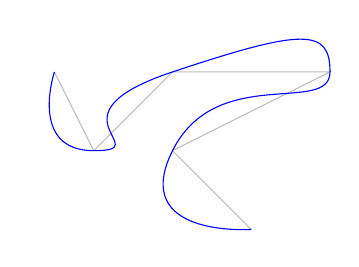
\begin{tikzpicture}
			\draw [gray!50]  (-0.5, 1) -- (0,0) -- (1,1) -- (3,1) -- (1,0)  -- (2,-1);
			\draw [blue] plot [smooth, tension=2] coordinates {(-0.5, 1) (0,0) (1,1) (3,1) (1,0) (2,-1)};
	\end{tikzpicture}}{עקומה וקירוב לינארי שלה, שחוסם מלמטה את אורכה}

	\textbf{דוגמה. }נתבונן בעקומה $[-1, 1] \to \R^{2}$ המוגדרת ע''י:
	\[ \cg(x) = (x, \sqrt{1 - x^{2}}) \]
	\fig{\begin{tikzpicture}
			\begin{axis}[
				axis equal image,
				xmin=-1.5, xmax=1.5,
				ymin=-0.5, ymax=1.5,
				ymajorgrids=true,
				xmajorgrids=true,
				grid style=dashed,
				]
				.. controls (axis cs:0.555,1) and (axis cs:1,0.555) .. (axis cs:1,0);
				\draw [blue] (axis cs:1,0) arc [start angle=0, end angle=180, radius=100];
			\end{axis}
	\end{tikzpicture}}{העקומה $\cg$ המוגדרת בדוגמה. אורך מעגל היחידה הוא $2\pi$}

	\clm{$\cg$ היא עקומה בעלת אורך סופי, וכן $2 \le L(\cg) \le 4$. }\begin{proof}
		מספיק להראות:
		\begin{enumerate}
			\item קיימת חלוקה $\Pi$ של $[-1, 1]$ עם $\ml(\cg, \Pi) = 3$
			\item לכל חלוקה $\Pi$ של $[-1, 1]$ עם $\ml(\cg, \Pi) \le 4$
		\end{enumerate}
		פרטים יעלו למודל.
	\end{proof}
	\defi{$\pi := L(\cg)$ כאשר $\cg$ העקומה המוגדרת לעיל. }

\subsection{הגדרת אינטגרל רימן}
\subsubsection{סכומי רימן}
	זה עתה הגדרנו אורך של עקומה, אובייקט רציף $[0, 1] \to \R$, באמצעות התבוננות על כל החלוקות ולקיחת הסופרמום שלהם. הדרך בה נגדיר את ''השטח מתחת לגרף של $f$``, הוא מושג האינטגרל, מזכיר במקצת את מה שזה עתה עשינו בעבור עקומות, אם כי למקרה זה יש דקויות רבות יותר. 

	נתחיל מתיאור יוריסטי: ''שטח מתחת לגרף``. עבור פונקציה $f \co [a, b] \to \R$, נסמן:
	\[ \int^{b}_a \dequad \ f = \int^{b}_a \dequad\ f(x)\dx = \int^{b}_a \dequad \ f(t) \dt = \int \Is f \]
	כאשר ''מתחת לגרף`` השטח שלילי. לעיתים נרצה לתאר אינטגרל של פונקצייה על כל $\R$, או על קטע חצי־פתוח $(0, 1]$ (לדוגמה במקרה של $\frac{1}{x^{2}}$), ולמושג הזה נקרא \textit{אינטגרל לא אמיתי}. 
	נתארו גם בצורה יוריסטית; נתבונן בפונקציה $f(x) = \frac{1}{x^2}$ בקטע $f \co [1, \inft) \to \R$. יש לנו כאן בעיה – הפונקציה מוגדרת על קטע (קרן) לא חסום. עתה נתבונן בפונקציה $f(x) = \frac{1}{\sqrt x} = x^{-\frac{1}{2}}$, שמוגדרת על קטע סופי $f \co (0, 1] \to \R$. כאן אומנם הפונקציה מוגדרת על קטע סופי, אך ב־$0$ היא שואפת לאינסוף, גם אם השטח לכאורה סופי. הפתרון הוא לקחת גבול על אינטגרל הרימן של הפונקציה (שזה מושג האינטגרל שנגדיר לקטעים סגורים).

	\exe{נתון מלבן $a \times b$, מחולק למלבנים $a_i \times b_i$, כאשר $i \in [n]$. אז:
	\[ ab = \sum_{i = 1}^{n}a_ib_i \]}
	למה התרגיל הזה חשוב? כי אם נתבסס על הקונספט של ''שטח מלבן`` (שהוא ידוע להיות $a \cdot b$, אורך כפול רוחב) חשוב לראות שזה מכבד את מה שהיינו ''מצפים`` מהגדרה של שטח – שהשלם שווה לסך חלקיו.

	להלן הרעיון מאחורי אינטגרל רימן: בהינתן פונקציה וגרפה, נבחר חלוקה של הקטע, ''נדגום`` את הערך של הפונקציה בנקודה שבחרנו, וניקח את הערך בנקודת הדגימה להיות הגובה של המלבן. לבחירה הזו נקרא ''תיוג`` או ''נקודות מתאימות``.

	\defi{\textit{חלוקה מתויגת} (באנגלית tagged partition, ברשימות ''חלוקה+נקודות מתאימות``) של הקטע $[a, b]$
		היא זוג $(\Pi, \{t_i\})$ כאשר $\Pi\co a = x_0 < x_1 < \cdots < x_n = b$ חלוקה של הקטע $[a, b]$, וכן תיוג $t_i \in [x_{i - 1}, x_i]$ לכל אחד מ־$i \in [n]$ קטעי החלוקה. אז \textit{סכום רימן} של הפונקציה $f \co [a, b] \to \R$ ביחס לחלוקה המתויגת $\{t_i\}_{i = 1}^{n}$ הוא:
		\[ S(f, \pi, \{t_i\}) := \sumnio f(t_i)\Delta x_i \]}

	\textbf{דוגמה. }\fig{\begin{pspicture}(-0.5,-1.5)(10,1.5)
			\psaxes[ticks=none,labels=none]{->}(0,0)(-1,-1.5)(10,1.5)
			\psStep[linecolor=black!70,StepType=upper,algebraic,fillstyle=solid,fillcolor=blue!10](0,9){20}{sqrt(x)*sin(x)*cos(x)}
			\psplot[plotpoints=100,linewidth=1pt,algebraic]{0}{9.5}{sqrt(x)*sin(x)*cos(x)}
	\end{pspicture}}{סכומי רימן של $\sqrt x\sinx\cosx$, עם נקודות מתאימות בסוף החלוקה ($t_i = x_{i}$)}
	

	\exe{ציירו חלוקה מתויגת של הקטע $[0, 1]$ עם שלושה תתי־קטעים באורכים שאינם כולם שווים, ועם $t_2 = t_3$. }

	עתה נתעסק עם שתי דוגמאות \textit{חשובות} שבהחלט יכולות להופיע בבחינה. נתבונן בפונקציה:
	\begin{align*}
		f \co [a, b] \to \R && f(x) = \begin{cases}
			5 & x = a \\
			15 & x \neq a
		\end{cases}
	\end{align*}
	נתבונן בסכום רימן ביחס לחלוקה כלשהי:
	\[ S(f, \Pi, \{t_i\}) = \sum_{i = 1}^{n}f(t_i)\Delta x_i = f(t_1)\Dg x_1 + \sum_{i = 2}^{n}\underbrace{f(t_i)}_{5}\Delta x_i \]
	כתלות בבחירה של נקודת הדגימה $t_1$, אם $t_1= a$ אז הסכום יוצא $10 \Delta x_i + 5(b - a)$, אחרת זה יוצא $5(b - a)$. לכן, נקבל:
	\[ \sof{S(f, \Pi, \{t_i\}) - 5(b - a)} \le 10 \Dg x_i \le 10 \, \lg(\Pi) \]

	יש לנו דוגמה חשובה נוספת: פונקציית דיריכלה. 

	\textbf{דוגמה. }נתבונן בפונקציית דיריכלה:
	\[ D(x) = \begin{cases}
		1 & x \in \Q \\
		0 & x \notin \Q
	\end{cases} \]
	ניקח חלוקה מתויגת $(\Pi, \{t_i\})$ של קטע $[a, b]$.
	\begin{itemize}
		\item אם לכל $i \in [n]$ מתקיים $t_i \in \Q$ (בהכרח קיים תיוג כזה, מצפיפות), אז:
		\[ S(f, \Pi, \{t_i\}) = \sumnio 1 \Delta x_i = b - a \]
		\item אם לכל $i \in [n]$ מתקיים $t_i \notin \Q$ אז:
		\[ S(f, \Pi, \{t_i\}) = \sumnio 0 \Delta x_i = 0 \]
	\end{itemize}
	נבחין שלא משנה עד כמה החלוקה $\Pi$ תהיה עדינה, תמיד נוכל לבחור תיוג כך שסכום רימן הוא $0$ ותיוג אחר כך שסכום רימן יהיה $1$. זו הסיבה שפונקציית דיריכלה תקרא \textit{לא אינטגרבילית רימן}. 


\subsubsection{אינטגרל רימן}
	\defi{נתונה פונקציה $f \co [a, b] \to \R$. נאמר ש־$f$ \textit{\href{https://eincyclopedia.org/wiki/\%D7\%A4\%D7\%95\%D7\%A0\%D7\%A7\%D7\%A6\%D7\%99\%D7\%94\_\%D7\%90\%D7\%99\%D7\%A0\%D7\%98\%D7\%92\%D7\%A8\%D7\%91\%D7\%99\%D7\%9C\%D7\%99\%D7\%AA}{אינטגרבילית} רימן עם אינטגרל שווה ל־$I$} אם\footnote{בהגדרות, ''אם`` זה ''אם ורק אם``, כי ברור ששני הכיוונים נדרשים} לכל $\eg > 0$ קיימת $\dg > 0$  כך שלכל חלוקה מתויגת $(\Pi, \{t_i\})$ של $[a, b]$, עם מדד עדינות $\lg(\Pi) < \dg$, מתקיים:
	\[ \sof{S(f, \Pi, \{t_i\}) - I} < \eg \]
	אם זה קורה, נאמר ש־$I$ \textit{האינטגרל המסויים} של $f$ בקטע $[a, b]$. }

	במילים אחרות, לכל אפסילון, עם מספר מסוים לעידון, אז כל חלוקה ותיוג יהיו בסביבת $\eg$ של ערך האינטגרל.

	\noti{מסמנים $\int^{b}_af = \int^{b}_af(x)\dx = I$}
	\defi{הפונקציה $f$ נקראת \textit{אינטגרבילית} אם קיים $I$ כך ש־$\int^{b}_a f = I$. }

	\rmark{$I$ איננו במובן הרחב, כלומר $I \in \R$. }

	\begin{Exercise}[''לא יכולה  להגזים בכמה הוא חשוב``]
		רשמו את השלילה של הביטוי $\int^{b}_a f = I$.
	\end{Exercise}

	\rmark{נניח שהאינטגרל של $f$ איננו שווה ל־$I$. יש שתי סיבות, מאוד שונות, לסיבה שזה קורה:
	\begin{itemize}
		\item $\int^{b}_a f = I' \neq I$
		\item $f$ איננה אינטגרבילית רימן בקטע $[0, 1]$.
	\end{itemize}}
	בהמשך נראה קריטריונים לאינטגרביליות של דורשים לדעת מי זה בדיוק $I$ (באופן דומה לכך שיודעים שפונקציה מתכנסת לאנשהו באמצעות קריטריון קושי, אך לא יודעים לאן).

	נציין את המשפטים הייסודים של החדו''א. לא נוכיח אותם כרגע, הם בחומר לעוד איזה חודש, אבל הם מה שיקשור את התיאוריה של ההרצאה לשבועיים הראשונים של התרגול (שכרגע יראו לא קשורים בעליל). ידועים גם בתור משפטי ניוטון־לייבניץ\footnote{המלחמה בנוגע מי הגיע למשפטים קודם, נמשכת עד היום. }

	בהינתן $f, F \co [a, b] \to \R$:
	\begin{enumerate}
		\item ''תחת הנחות מסוימות`` (\href{https://eincyclopedia.org/wiki/\%D7\%A4\%D7\%95\%D7\%A0\%D7\%A7\%D7\%A6\%D7\%99\%D7\%94\_\%D7\%A1\%D7\%99\%D7\%9E\%D7\%A4\%D7\%98\%D7\%99\%D7\%AA}{פונקציה סימפטית מספיק}), אם $F(x) = \int^{x}_a f(t) \dt$, אז $F'(x) = f(x)$.
		\item ''תחת הנחות מסוימות``, אם $F'(x) = f(x)$, אז $F(x) = F(a) + \int^{x}_af(t)\dt$
	\end{enumerate}
	זה מסביר למה המושג הבא כל־כך חשוב לחישובי אינטגרלים:
	\defi{לפונקציות ממשיות $f, F \co I \to \R$ על קטע $I \subset \R$, אז $F$ נקראת \textit{פונקציה קדומה של $f$ על קטע\footnote{לשימושנו, קבוצה סגורה. } $I$} אם $\forall x \in I \co F'(x) = f(x)$, כאשר בקצוות הקטע (אם יש כאלו) מדובר על נגזרת חד־כיוונית. }
	נעבוד בתרגולים למצוא פונקציות קדומות, כי הן בתורן יאפשרו לחשב אינטגרלים מסוימים, באמצעות המשפט היסודי.

	\defi{\textit{האינטגרל הלא מסויים של $f$} הוא \textbf{קבוצת} הפונקציות הקדומות של $f$. }
	בקורס ''פונקציות ממשיות`` נגדיר מושג אינטגרל רחב יותר, שנקרא \textit{אינטגרל לבג}, וניתן להגדיר אותו גם מחוץ ל־$\R$. כרגע אנחנו עובדים עם אינטגרל רימן.


	\begin{Exercise}[תרגיל חזרה על חדו''א 1א]
		\begin{enumerate}
			\item יהיו $A, B \subset \R$ קבוצות ממשיים. נגדיר $A + B = \{a + b \mid a\in A \land b \in B\}$. הוכיחו:
			\[ \sup (A + B) = (\sup A) + (\sup B) \]
			\item יהיו $A \subset \R$ קבוצת ממשיים, וכן $\lg > 0$. נגדיר $\lg A = \{ \lg a \mid a \in A\}$. הוכיחו $\sup(\lg A) = \lg \sup A$.
			\item יהיו $A, B \subset \R$ קבוצות חסומות. הוכיחו:
			\[ \sup (A \cup B) = \max\{\sup A, \sup B\} \]
			\item יהיו $A, B \subset \R$ חסומות. הוכיחו:
			\begin{enumerate}[A.]
				\item \hfil $\sup A \le \inf B \iff \forall a \in A, b \in B\co a \le b$
				\item \hfil $\sup A \ge \inf B \iff \forall \eg > 0 \exists a \in A, b \in B \co b - a < \eg$
			\end{enumerate}
			\item $A \subset B$ חסומה, אז:
			\[ \sup A - \inf A = \sup\{a - b \mid a, b \in A\} \]
		\end{enumerate}
	\end{Exercise}
	הרבה מהדברים שנעשה בשעתיים הקרובות ידרשו את זה, וזה יתחבא למטה.

\subsubsection{דוגמאות חישוביות}
	נתבונן בפונקציה:
	\begin{align*}
		f \co [a, b] \to \R && f(x) = \begin{cases}
			15 & x = a \\
			5 & a < x \le b
		\end{cases}
	\end{align*}
	\clm{$\int^{b}_af = 5(b-a)$}

	בהגדרה הקודמת שלנו לאינטגרל רימן, נדרשנו לדעת מה הערך של האינטגרל כדי להיות מסוגלים להוכיח אינטגרביליות.
	\begin{proof}
		יהי $\eg > 0$. יהי $\dg  = \dg_\eg = ?$ (בדיעבד אחרי כן נדע להשלים את ה־$\dg$, אך כתלות ב־$\eg$ בלבד) ותהי חלוקה מתויגת $(\Pi, \{t_i\})$ של הקטע $[a, b]$. נניח שמדד העדינות $\lg(\Pi) < \dg$. יש להוכיח $\sof{S(f, \Pi, \{t_i\}) - 5(b - a)} < \eg$. נזכר שחישבנו בעבור הפונקציה לעיל בשיעור הקודם ש־:
		\[ \sof{S(f, \Pi, \{t_i\}) - 5(b-a)} \le 10 \cdot \lg(\Pi) < 10 \delta = \cdots \]
		מכאן, שבעבור $\dg = \frac{\eg}{10}$ נקבל:
		\[ \cdots = \eg \]
		כנדרש.
	\end{proof}

	נזכר בתרגיל (''שאתם לא מבינים כמה הוא חשוב וכמה סטודנטים מתקשים בו``. ''אם אתם מתקשים, תבואו לשעת הקבלה. אם אתם לא מתקשים, תבואו לשאול משהו אחר. לא ממליצה לשאול את ה־AI, הוא יכניס לכם רעש``). יעל מזכירה ש־AI יכול מאוד לעזור, אבל צריך להיות במצב (מתמטית) שאנו יודעים להנחות אותו לעזור לנו. התרגיל – השלילה של הביטוי ''$f$ איננה אינטגרבילית``.

	\clm{פונקציית דיריכלה איננה אינטגרבילית, על אף תת־קטע סגור $[a, b]$ ($a < b$). }
	\begin{proof}
		נזכר בהגדרתה:
		\[ D(x) = \begin{cases}
			1 & x \in \Q \\
			0 & x \notin \Q
		\end{cases} \]
		נקבע קטע $[a, b]$. נניח בשלילה שקיים $I \in \R$  כך ש־$\int^b_a D(x) \dx = I$. נבחר $\eg = ?$ (נשלים אחרי כן מה הוא, כתלות ב־$I$ ו־$[a, b]$ בלבד) ותהי $\dg = \dg_e > 0$ המתאימה ל־$\eg$ ע''פ הגדרת אינטגרל רימן. נבחר $\Pi$ חלוקה של הקטע $[a, b]$, עם מדד עדינות $\lg(\Pi)$ (תרגיל: הוכיחו שקיימת כזו בהכרח כזו). מבחירת $\dg$, לכל תיוג של $\Pi$ נאמר $\{t_i\}$, מתקיים ש־: $\sof{S(f, \Pi, \{t_i\}) - I} < \eg$. מצפיפות הרציונליים והאי־רציונליים:
		\begin{itemize}
			\item קיים תיוג $\{t_i\}$ עם $t_i \in \Q$ (עבורו: סכום רימן הוא $b - a$, הוכחנו בשיעור הקודם)
			\item קיים תיוג $\{t'_i\}$ עם $t_i \notin \Q$ (עבורו: סכום רימן הוא $0$ הוכחנו בשיעור הקודם)
		\end{itemize}
		עבור התיוג הראשון נקבל $\sof{(b - a) - I} < \eg$ ועבור התיוג השני נקבל $\sof{0 - I} < \eg$. נבחר בדיעבד (וכתלות ב־$[a, b]$ בלבד) את $\eg = \frac{b - a}{3}$. מא''ש המשולש:
		\[ \sof{b - a} \le \sof{(b - a) - I} + \sof I < 2 \eg < b - a\quad \bot \]\envendproof
	\end{proof}



\subsubsection{חסימות ואינטגרביליות}
	אנחנו קצת בבעיה. כדי להראות שפונקציה היא אינטגרבילית, היינו צריכים ''להחזיק $I$ ביד`` ולדעת מה הערך של האינטגרל. עתה נמצא ל''מסע`` כדי למצוא תנאים הכרחיים, מספיקים, ושקולים להיות פונקציה אינטגרבילית, בלי לדעת מה הוא ה־$I$.

	\noti{\hfil $R([a, b]) := \{f \co [a, b] \to \R \mid \text{אינטגרבילית} f\}$}
	לשימושנו, \textbf{אינטגרבילית=אינטגרבילית רימן}. יש מושגי אינטגרציה אחרים (כמו אינטגרל לבג) שלא רלוונטיים בעבורנו. 
	
	\renewcommand{\footrule}{\rule{\linewidth-26pt}{0.25pt}\vspace{-5pt}}

	\theo{נניח $f \in \rim$, אז $f$ חסומה. }
	לדוגמה, הפונקציה: 
	\begin{align*}
		f \co [0, 1] \to \R && f(x) = \begin{cases}
			\frac{1}{\sqrt x} & 0 < x \le 1 \\
			0 & x = 0
		\end{cases}
	\end{align*}
	כאשר נלמד על אינטגרל לא אמיתי, נמצא משמעות לשטח מטחת לגרף, אבל $f$ איננה אינטגרבילית רימן. נפנה להוכיח את המשפט:
	\begin{proof}[הוכחת המשפט]
		נניח $f \co [a, b] \to \R$ אינטגרבילית רימן. מכאן שקיים $I \in \R$ כך ש־$\int^b_a f = I$. יהי $\eg$, נבחר אותו להיות $\eg = 1$ (זה לא קריטי לאיזה ערך מקבעים אותו). תהי $\dg > 0$ מתאימה ל־$\eg$ בהתאם להגדרת אינטגרל רימן. נבחר $\Pi = \{x_i\}_{i = 0}^{n}$ חלוקה של $[a, b]$ עם מדד עדינות $\lg(\Pi) < \dg$ (זכרו, יש להוכיח שקיימת כזו, תרגיל שנשאר לבית). נקבע תיוג $\{t_i\}_{i = 1}^{n}$ כלשהו של $\Pi$.

		''נחלק`` את הקטע $[a, b]$ לקטעים קטנים ונדרוש שהיא תהיה חסומה על כל אחד מקטעי הביניים בנפרד. יהי $k \in \{1, \dots n\}$, וננסה להוכיח חסימות ב־$[x_{k - 1}, x_k]$. נתבונן בתיוגים $\{t'_i\}_{i = 1}^{n}$ מהצורה:
		\[ t'_1 \dots t'_n = \underbrace{t_1 \dots t_{k - 1}}_{\ \!\text{קבועים}}, \overbrace{t}^{\mathclap{t \in [x_{k - 1}, x_k]}}, \underbrace{t_{k + 1}, \dots, t_n}_{\ \!\text{קבועים}} \]
		מהגדרת אינטגרל רימן, סכום רימן בעבור כל תיוג בסביבת $\eg$ של $I$, כלומר:
		\[ I - \eg < \underbrace{S(f, \Pi, \{t'_i\})}_{\mathclap{=f(t)\Delta x_k + \sum_{i \neq k}f(t_i)\Delta x_i}} < I + \eg \]
		נבחין ש־$\sum_{i \neq k} f(t_i)\Delta x_i$ קבוע ביחס לבחירת $k$, ונסמנו $C_k$. לכן לכל $t \in [x_{k - 1}, x_k]$ מתקיים:
		\begin{gather*}
			I - \eg - C_k < f(t) \Delta x_k < T + \eg - C_k \\
			\frac{I - \eg - C_k}{\Delta x_k} < f(t) < \frac{I + \eg - C_k}{\Delta x_k}
		\end{gather*}
		''לכן $f|_{[x_{k - 1}, x_k]}$ חסומה, והטוש הזה הלך לעולמו``.

		סה''כ $f$ חסומה על כמות סופית של קטעים סגורים שמכסים את $[a, b]$, כלומר היא חסומה.
	\end{proof}

	שימו לב! פונקציה חסומה לא חייבת להיות אינטגרבילית, לדוגמה, תנאי דרבו. חסימות הוא תנאי הכרחי, אך לא מספיק, לאינטגרביליות.

\subsection{סכומי דרבו}
\subsubsection{הגדרות בסיסיות}
	אם רוצים להמנע מבחירת תיוג, בהינתן חלוקה, אפשר לקחת את האינפימום והסופרמום של הפונקציה על אותו קטע חלוקה. גובה המלבנים שיבחר על ידי התיוגים יהיו חסומים ע''י זה. פורמלית:
	\defi{תהי $f \co [a, b] \to \R$ חסומה. תהי $\Pi = \{x_i\}_{i = 1}^{n}$ חלוקה של $[a, b]$, כלומר $a = x_0 < x_1 < \cdots < x_n = b$. לכל $i$, נגדיר:
	\[ M_i := \sup_{\mathclap{[x_{i - 1}, x_i]}} f \quad\quad m_i := \inf_{\mathclap{[x{i -1}, x_i]}} f \]
	(שימו לב שזה מוגדר רק בגלל שהנחנו $f$ חסומה).
	}

	\defi{בהינתן ההנחות מההגדרה הקודמת, נגדיר את \textit{סכום דרבו העליון} ו\textit{סכום דרבו התחתון} להיות:
	\begin{align*}
		\ol{\Sigma}(f, \Pi) = \sum_{i = 1}^{n} M_i\Delta x_i && \dard(f, \Pi) := \sum_{i = 1}^{n}m_i \Delta x_i
	\end{align*}}

	\fig{\begin{pspicture}(-0.5,-3)(10,3)
			\psaxes[ticks=none,labels=none]{->}(0,0)(-1,-2.5)(10,3)
			\psplot[plotpoints=100,linewidth=1.5pt,algebraic]{0}{9.5}{sqrt(x)*sin(x)}
			\psStep[linecolor=green,StepType=supremum,fillstyle=hlines,algebraic](0,9.5){20}{sqrt(x)*sin(x)}
			\psStep[linecolor=blue,StepType=infimum,fillstyle=vlines,algebraic](0,9.5){20}{sqrt(x)*sin(x)}
	\end{pspicture}}{סכומי דרבו עליונים בירוק, סכומי דרבו תחתונים בכחול, בעבור חלוקה ''אחידה``}

	\lem{תהי $f \co [a, b] \to \R$ חסומה, ו־$\Pi$ חלוקה של $[a, b]$. אז	לכל תיוג $\{t_i\}$ של החלוקה $\Pi$, מתקיים:
		\[ \dard(f, \Pi), S(f, \Pi, \{t_i\}) \le \daru(f, \Pi) \]
	}
	\begin{proof}
		לכל $i \in [n]$, מתקיים $m_i \le f(t_i) < M_i$. נכפיל ב־$\Delta x_i$ את הא''שים ונסכם על $i$. נקבל:
		\[ \dard(f, \Pi) = \sumnio m_i\Delta x_i \le \sum_{i = 1}^{n}f(t_i)\Delta x_i \le \sum_{i = 1}^{n} M_i \Delta x_i = \daru(f, \Pi) \]
		כנדרש.
	\end{proof}
	\lem{תהי $f \co [a, b] \to \R$ חסומה, וכן $\Pi$ חלוקה של $[a, b]$. אז:
	\begin{align*}
		\daru(f, \Pi) &= \sup\ccb{S(f, \Pi, \{t_i\}) \mid \Pi \ \text{תיוג של} \ \{t_i\}} \\
		\dard(f, \Pi) &= \inf\ccb{S(f, \Pi, \{t_i\}) \mid \Pi \ \text{תיוג של} \ \{t_i\}}
	\end{align*}}
	ברשימות של שירי יש הוכחה קונקרטית עבור $\daru$, בעוד ההוכחה בעבור $\dard$ אמורה להופיע בתרגיל הבית (''אתם מעתיקים מהרשימות של שירי, וכל דבר עליון, תחתון``). לב הטיעון יושב בתוך (הכללה באינדוקציה של) תרגיל הפתיחה של ההרצאה הזו. אנחנו גם נוכיח בעבור $\daru$:
	\begin{proof}
		נגדיר $A_i = \{f(t_i) \mid t_i \in [x_{i - 1}, x_i]\}$ (כלומר $A_i = f([x_{i - 1}, x_i])$). אז:
		\begin{multline*}
			\Sigma A := \ccb{S(f, \Pi, \{t_i\}) \mid \Pi \ \text{תיוג של} \ \{t_i\}} = \ccb{\sum_{i = 1}^{n}f(t_i)\Delta x_i \mid \forall i \co t_i \in [x_{i - 1}, x_i} = \ccb{\sumnio a_i \Delta x_i \mid a_i \in A_i} \\
			= (\Delta x_1)A_1 + \cdots + (\Delta x_n) A_n
		\end{multline*}
		המושגים של ''לחבר קבוצות`` ו''להכפיל קבוצה במספר`` נתונים בתרגיל הפתיחה, שם נמצא עיקר התוכן. ברשימות של שירי זה כתוב יותר מפורש. \\
		נזכר שבעצם יש להוכיח ש־$\daru(f, \Pi) = \sup \Sigma A$. מהשוויונות לעיל נקבל ש־:
		\begin{align*}
			\sup \Sigma A &= \sup((\Delta x_1)A_1 + \cdots + (\Delta x_n)A_n) \\
			&= \Delta x_1 \underbrace{\sup A_1}_{\smash{M_1}} + \cdots + \Delta x_n \underbrace{\sup A_n}_{\smash{M_n}} \\
			&= \sum_{i = 1}^{n}M_i\Delta x_i = \daru(f, \Pi)
		\end{align*}
	\end{proof}

	\begin{Theorem}[מונוטוניות של סכומי דרבו ביחס לעידון החלוקות]
		תהי $f \co [a, b] \to \R$ חסומה. יהיו שתי חלוקות $\Pi_1 \subset \Pi_2$ חלוקות של $[a, b]$. אז:
		\[ \dard(f, \Pi_1) \le \dard(f, \Pi_2) \le \daru(f, \Pi_2) \le \daru(f, \Pi_1) \]
	\end{Theorem}
	אינטואיטיבית: כשמעדנים את החלוקה, סכום דרבו העליון והתחתון מתקרבים זה לזה, אך לא בהכרח משתווים. היינו רוצים שהם יתקרבו אל האינטגרל. שימו לב: חצי מהא''שים במשפט ידועים מהמשפט הקודם.
	\begin{proof}[הוכחה עבור סכום דרבו עליון, במקרה הפרטי של $\Pi_2 = \Pi_1 \uplus \{p\}$]
		נרשום $\Pi_1 \co a = x_0 < x_1 < \cdots < x_n = b$. ישנו $k$ כך ש־$x_{k - 1} < p < x_k$. נסמן $M_i = \sup_{[x_{i - 1}, x_i]} f$, וכן $M'_k = \sup_{[x_{k - 1}, p]} f$ ו־$M''_k = \sup_{[p, x_k]}f$. אז:
		\[ \daru(f, \Pi_2) = \sum_{i \neq k} M_i \Delta x_i  + \underbrace{\overbrace{M'_k}^{\le M_k}(p - x_{k - 1}) + \overbrace{M''_k}^{\le M_k}(x_k - p)}_{\le M_k(x_k - x_{k -1})} \le M_k\Delta x_k + \sum_{i \neq k} M_i\Delta x_i = \daru(f, \Pi_1) \]
		כנדרש.
	\end{proof}
	הוכחת המקרה הכללי באינדוקציה על הנקודות שנוספו לחלוקה (זכרו, חלוקות הן סופיות). הוכחה עבור סכום דרבו תחתון מדואליות.

	\begin{Collary}
		לכל שתי חלוקות $\Pi_1, \Pi_2$ של $[a, b]$, תמיד $\dard(f, \Pi_1) \le \daru(f, \Pi_2)$.
	\end{Collary}
	\begin{proof}
		האיחוד $\Pi_3 := \Pi_1 \cup \Pi_2$ הוא עידון של $\Pi_1$ ושל $\Pi_2$ (עידון משותף). מהמשפט הקודם:
		\[ \dard(f, \Pi_1) \le \dard(f, \Pi_3) \le \daru(f, \Pi_3) \le \daru(f, \Pi_2) \]
		כנדרש.
	\end{proof}
	זו מסקנה נחמדה, שאומרת שקבוצת כל סכומי הדרבו העליונים חסומה מלמטה (ע''י סכום דרבו תחתון כלשהו) ולהפך. זה אומר שקיים לה סופרמום.

	\defi{תהי $f \co [a, b] \to \R$ חסומה. נגדיר:
	\begin{itemize}
		\item אינטגרל דרבו עליון: \hfill $\displaystyle \Idaru(f) := \inf \ccb{\daru(f, \Pi) \mid [a, b] \ \text{חלוקה של} \ \Pi}$
		\item אינטגרל דרבו תחתון: \hfill $\displaystyle \Idard(f) := \sup \ccb{\dard(f, \Pi) \mid [a, b] \ \text{חלוקה של} \ \Pi}$
	\end{itemize}}

	\defi{$f$ \textit{אינטגרבילית דרבו} אם $\Idard(f) = \Idaru(f)$. אם זה קורה, $I(f) = \Idard(f) = \Idaru(f)$ נקרא \textit{אינטגרל דרבו}. }

	\theo{עבור $f \co [a, b]\to \R$, $f$ אינטגרבילית רימן אמ''מ $f$ חסומה וגם $f$ אינטגרבילית דרבו. אם תנאים אלו מתקיימים, אז $\int^{b}_af = I(f)$. }

	\rmark{אינטגרל דרבו העליון והתחתון לא מוגדרים במידה ו־$f$ איננה חסומה, ולכן זו תמיד תתווסף כהנחה למשפטים הדורשים אינטגרל דרבו עליון או תחתון. }

	\begin{Theorem}[קריטריון דרבו]
		$f \co [a, b] \to \R$ אינטגרבילית אמ''מ $f$ חסומה וגם לכל $\eg > 0$, כך שלכל חלוקה $\Pi$ של $[a, b]$, אם $\lg(\Pi) < \dg$ אז $\daru(f, \Pi) - \dard(f, \Pi) < \eg$.
	\end{Theorem}
	\begin{Theorem}[קריטריון דרבו המשופר]
		$f \co [a, b] \to \R$ אינטגרבילית אמ''מ $f$ חסומה וגם לכל $\eg > 0$ קיימת חלוקה $\Pi$ של $[a, b]$ עם $\daru(f, \Pi) - \dard(f, \Pi) < \eg$.
	\end{Theorem}

	\begin{proof}[הוכחת קריטריון דרבו הרגיל, החלק של ''רק אם``]
		נניח ש־$f$ אינטגרבילית רימן עם $\int^{b}_a f = I$. כבר הראינו ש־$f$ חסומה. יהי $\eg > 0$. נבחר $\hat \eg = ?$ (נבחר בהמשך את ערכו). בהתאם להגדרת אינטגרל רימן, תהי $\dg$ שמתאימה ל־$\hat \eg$. תהי $\Pi$ חלוקה עם $\lg(\Pi) < \dg$. מבחירת $\dg$, לכל תיוג $\{t_i\}$ של החלוקה, נקבל:
		\[ I - \hat \eg < S(f, \Pi, \{t_i\}) < I + \hat \eg \]
		מטענה קודמת, ומשום שספורמום מכבד א''ש חלש, נקבל מיידית ש־:
		\[ I - \hat \eg \le \int_{\{t_i\}} S(f, \Pi, \{t_i\}) = \dard(f, \Pi) \le \daru(f, \Pi) = \sup_{\{t_i\}} S(f, \Pi, \{t_i\}) \le I + \eg \]
		נובע:
		\[ \daru(f, \Pi) - \dard(f, \Pi) \le 2 \hat \eg \]
		מכאן שעבור בחירת $\hat \eg = \frac{\eg}{3}$ נקבל את הנדרש.
	\end{proof}
	הכיוון ''אם`` השני – מהרשימות של שירי.

	\begin{Exercise}
		תהא פונקציה $f \co [a, b] \to \R$ ומספר $I \in \R$, וכן סדרת חלוקות מתויגות $(\Pi_k, \{t^{(k)_{\{t_i\}}}\})$ של $[a,b]$ שמדדי העדינות שלהן מקיימים $\lg(\Pi_k) \rrr{k \to \inft} 0$. הוכיחו:
		\begin{enumerate}
			\item אם $\int^{b}_a f = I$ אז $S(f, \Pi_k, \{t_i^{(k)}\}) \rrr{k \to \inft} 0$.
			\item נניח $S(f, \Pi_k, \{t_i^{(k)}\}) \rrr{k \to \inft} 0$. האם בהכרח $\int^{b}_a = I$? [רמז: אפריורי לא יודעים בהכרח ש־$f$ אינטגרבילית]
		\end{enumerate}
	\end{Exercise}


\subsubsection{אינטגרביליות דרבו ואינטגרביליות רימן}
	נסכם את שלושת המשפטים האחרונים שראינו לכדי שקילות אחת: 
	\theo{נתונה פונקציה ממשית $f \co [a, b] \to \R$. עבור פונקציה כזו, התנאים הבאים שקולים:
		\begin{enumerate}
			\item קיים $I \in \R$ כך שלכל $\eg > 0$ קיים $\dg > 0$ כך שלכל חלוקה מתוייגת $(\Pi, \{t_i\})$ של $[a, b]$, אם $\lg(\Pi) < \dg$, אז $\sof{S(f, \Pi, \{t_i\}) - I} < \eg$.
			\item הפונקציה $f$ חסומה, וגם לכל $\eg > 0$, קיימת $\dg > 0$ כך שלכל חלוקה $\Pi$ של $[a, b]$, אם $\lg(\Pi) < \lg$, אז $\daru(f, \Pi) - \dard(f, \Pi) < \eg$.
			\item $f$ חסומה, וגם לכל $\eg > 0$ קיימת חלוקה $\Pi$ של $[a, b]$ כך ש־$\daru(f, \Pi) - \dard(f, \Pi) < \eg$
			\item $f$ חסומה, וגם $\Idard(f) = \Idaru(f)$.
	\end{enumerate}}

	\exe{התאימו בין השקילויות לעיל לשקילות הבאה:
	\begin{enumerate}
		\item $f$ אינטגרבילית רימן
		\item $f$ מקיימת את התנאי בקריטריון דרבו
		\item $f$ מקיימת את התנאי בקריטריון דרבו המשופר
		\item $f$ אינטגרבילית דרבו
	\end{enumerate}}

	(רמז: הם לפי הסדר)

	בשיעור הקרוב נוכיח את השקילויות לעיל, ואז נפנה להסיק מהן מסקנות.

	\exe{שיעור שעבר הוכחנו ש־$1$ גורר את $2$. הוכיחו ש־$2$ גורר את $3$ (רמז: ההוכחה קלה, זהו רק מקרה פרטי). }

	\begin{proof}[הוכחה ש־$3 \to 4$]
		יהי $\eg > 0$. מההנחה $3$ קיימת חלוקה $\Pi$ כך ש־$\daru(f, \Pi) - \dard(f, \Pi) < \eg$. מצד שני, ידוע מהשיעור הקודם ומהגדרת אינטגרל דרבו עליון ותחתון:
		\[ \daru(f, \Pi) \le \Idard(f) \le \Idaru(f) \le \daru(f, \Pi) \]
		נובע ש־$\sof{\Idaru(f) - \Idard(f)} < \eg$, בעבור כל $\eg > 0$ שרירותי, ומכאן ש־$\Idaru(f)=\Idard(f)$ כנדרש.
	\end{proof}

	נסכם: הוכחנו שיעור שעבר $1 \to 2$, נתנו כתרגיל $2 \to 3$, ועתה הראינו $3 \to 4$. עתה נוכיח $4 \to 1$. מההנחה של 4 יש לנו אינטגרל דרבו, ונוכל להראות שהוא שווה לאינטגרל רימן.

	\begin{proof}[הוכחה ש־$4 \to 2$]
		נסמן $\Idard(f) = \Idaru(f) =: I$. אזי לכל חלוקה $\Pi$ של $[a, b]$ מתקיים:
		\[ (\mathrm{I}) \quad \dard(f, \Pi) \le I \le \daru(f, \Pi) \]
		כמו כן, לכל חלוקה מתויגת של הקטע:
		\[ (\mathrm{II})\quad \dard(f, \Pi) \le S(f, \Pi, \{t_i\}) \le \daru(f, \Pi) \]
		נחפש $\delta$ המתאימה ל־$\eg$ בהתאם להגדרה $2$ (נגדירה בהמשך). תהי $(\Pi, \{t_i\})$ חלוקה מתוייגת כלשהי עם $\lg(\Pi) < \dg$. מבחירת $\dg$, ידוע $\daru(f, \Pi) - \dard(f, \Pi) < \eg$. מ־$(\mathrm{I}), (\mathrm{II})$ fkunr
		$S(f, \Pi, \{t_i\})$ חסום בסביבת $\eg$ של $I$, כנדרש.
	\end{proof}
	נותרה לנו שקילות אחת להראות. לשם כך, נצטרך להגדיר כמה דברים.

	\defi{בהינתן $f \co J \to \R$ חסומה, \textit{תנודה} של $f$ ב־$J$ היא $\wg(f, J) := \sup_{J}f - \inf_J f$}
	\exe{הוכיחו כי
		\[ \wg(f) = \sup_{\mathclap{x, y \in J}}(f(x) - f(y)) = \sup\{\sof{f(x) - f(y) \mid x, y \in J}\} \]}

	\exe{עבור $J$ קטע פתוח, $x_0 \in J$, אז $f$ רציפה ב־$x_0$ אמ''מ $\wg(f, \; (x_0 - \dg, x_0 + \dg)) \rrr{\delta \to 0} 0$. }

	\defi{בהינתן $f \co [a, b] \to \R$ חסומה, ו־$\Pi$ חלוקה של $[a, b]$ נגדיר את \textit{תנודת דרבו של $f$ ביחס ל־$\Pi$} (או \textit{התנודה הכוללת של $f$ ביחס ל־$\Pi$}):
	\[ \wg(f, \Pi) := \sumnio \wg(f, [x_{i - 1}, x_i])\Delta x_i \]}

	\exe{הוכיחו כי:
	\[ \wg(f, \Pi) = \daru(f, \Pi) - \dard(f, \Pi) \]}

	\lem{בהינתן $\Pi, \Pi'$ חלוקות של $[a, b]$, כך ש־$\Pi' = \Pi \cup \{p\}$, מתקיים:
	\[ 0 \le \wg(f, \Pi) - \wg(f, \Pi') \le \lg(\Pi) \wg(f, [a, b]) \]}
	\begin{proof}
		נרשום $\Pi = \{x_0, \dots, x_n\}$, כך ש־$a = x_0 < \cdots < x_n = b$. תהי $k \in [n]$ כך ש־$x_{k  -1} < p < x_k$. אז:
		\[ \wg(f, \Pi) = \sum_{i \neq k} \wg(f, [x_{i - 1}, x_i])\Delta x_i + \wg(f, [x_{k - 1}, x_k])\Delta x_k \]
		וכן:
		\begin{align*}
			\wg(f, \Pi') &= \sum_{i \neq k} \wg(f, [x_{i - 1}, x_i]) \Delta x_i + \underbrace{\wg(f, [x_{k - 1}, p])(p - x_{k -1})}_{\wg(f, [x_{k - 1}, x_k])} + \underbrace{\wg(f, [p, x_k])(x_k - p)}_{\le \wg(f, [x_{k - 1}, x_k])} \\
			&\le \sum_{i \neq k} \cdots + \wg(f, [x_{k - 1}, x_k])\Big((p - x_{k - 1}) + (x_k - p)\Big) \\
			&= \wg(f, \Pi)
		\end{align*}
		נסכם:
		\begin{align*}
			\wg(f, \Pi) - \wg(f, \Pi') &= \wg(f, [x_{k - 1}, x_k])\Delta x_k - \cl{\text{שני ביטויים גדולים מ־0}} \\
			&\le \wg(f, [x_{k - 1}, x_k])\Delta x_k \le \wg(f, [a, b]) \cdot \lg(\Pi)
		\end{align*}
		כנדרש.
	\end{proof}
	\lem{נתונה $f \co [a, b] \to \R$ חסומה וחלוקות $\Pi, \Pi'$ של $[a, b]$ כך ש־$\Pi'$ מתקבלת מ־$\Pi$ ע''י הוספה של $m_0$ נקודות חלוקה. אז:
	\begin{alignat*}{9}
		(1) \quad 0 &\le \wg(f, \Pi) - \wg(f, \Pi') &\le m_0 \cdot \lg(\Pi) \; \wg(f, [a, b]) \\
		(2) \quad 0 &\le \daru(f, \Pi) - \daru(f, \Pi') &\le m_0 \cdot \lg(\Pi) \; \wg(f, [a, b]) \\
		(3) \quad 0 &\le \dard(f, \Pi) - \dard(f, \Pi') &\le m_0 \cdot \lg(\Pi) \; \wg(f, [a, b])
		\end{alignat*}}
	\begin{proof}
		באינדוקציה מהלמה הקודמת, אם $\Pi, \Pi'$ חלוקות ו־$\Pi''$ עידון של $\Pi$, אז $\wg(f, \Pi'') \le \wg(f, \Pi)$.
		\begin{enumerate}
			\item להוכחת $1$, נקבלת ישירות באינדוקציה מהלמה הקודמת על $m_0$. נרשום $\Pi' = \Pi'' \uplus \{p\}$ כאשר $\Pi''$ מתקבלת מ־$\Pi$ ע''י הוספת $m_0 - 1$ נקודות. נקבל:
			\[ \wg(f, \Pi) - \wg(f, \Pi') = \underbrace{\wg(f, \Pi) - \wg(f, \Pi'')}_{\mathclap{\le (m_0 - 1)\lg(\Pi)\wg(f, [a, b])}} + \underbrace{\wg(f, \Pi'') - \wg(f, \Pi')}_{\le \underbrace{\lg(\Pi'')}_{\le \lg(\Pi)}\wg(f, [a, b])} \le m_0 \lg(\Pi) \wg(f, [a, b]) \]
			\item[2, 3]ידוע:
			\[ 0 \le \underbrace{\cl{\daru(f, \Pi) - \daru(f, \Pi')}}_{\ge 0} + \underbrace{\cl{\dard(f, \Pi') - \dard(f, \Pi)}}_{\ge 0} = \wg(f, \Pi) - \wg(f, \Pi') \le \text{החסם לעיל} \]
		\end{enumerate}\envendproof
	\end{proof}

	\theo{תהי $f \co [a, b] \to \R$ חסומה. אז לכל $\eg < 0$ קיימת $\dg > 0$, כך שלכל חלוקה $\Pi$ של $[a, b]$, אם $\lg(\Pi) < \dg$ אז:
	\begin{align*}
		\daru(f, \Pi) - \eg \le \Idaru(f) && \Idard(f) \le \dard(f, \Pi) + \eg
	\end{align*}}
	\begin{proof}[הוכחה בעבור סכומי דרבו עליונים]
		נקבע $\Pi_0$ כך ש־:
		\[ \daru(f, \Pi_0) < \Idaru(f) + \frac{\eg}{2} \]
		יש כמות סופית של נקודות ב־$\Pi$, נסמנה $m_0$. תהי $\dg = ???$ שנשלים בהמשך.

		תהי $\Pi$ חלוקה עם $\lg(\Pi) < \dg$. תהי $\Pi'  =\Pi \cup \Pi_0$. נבחין ש־$\Pi'$ ניתנת ע''י הוספה של לכל היותר $m_0$ נקודות ל־$\Pi$.
		מהטענה שהוכחנו ו''ממונוטוניות`` של סכומי דרבו ביחס לעידון חלוקות:
		\[ \begin{WithArrows}
			\daru(f, \Pi) &\le \daru(f, \Pi') + m_0 \, \lg(\Pi) \wg(f, [a, b]) \Arrow{מונוטוניות} \\
			&\le \daru(f, \Pi_0) + m_0 \, \lg(\Pi) \wg(f, [a, b]) \Arrow[jump=2, down]{מבחירת $\!\,_0\Pi$} \\
			&\le \Idaru(f) + \frac{\eg}{2} + m_0 \, \smash{\underbrace{\lg(\Pi)}_{\le \dg}\wg(f, [a, b])} \\
			&< \daru(f) + \eg
		\end{WithArrows} \]
		כאשר השלמנו $\dg = \frac{1}{m_0\wg(f, [a, b])}$.
	\end{proof}

	עתה נחזור להוכיח $4 \to 1$ כדי להשלים את רצף הגרירות.
	\begin{proof}[הוכחה ש־$4 \to 1$]
		נתונה $f \co [a, b] \to \R$. נניח $f$ חסומה ו־$\Idard(f) = \Idaru(f)$. יהי $\eg > 0$. נבחר $\dg > 0$ שמתאימה ל־$\frac{\eg}{3}$ כמו בטענה שעכשיו הוכחנו. כלומר, לכל חלוקה $\Pi$, אם $\lg(\Pi) < \dg$ אז:
		\[ \dard(f, \Pi) - \frac{\eg}{3} \le I \le \dard(f, \Pi) +\frac{\eg}{2} \]
		תהי $(\Pi, \{t_i\})$ חלוקה מתוייגת עם $\lg(\Pi) < \dg$. מבחירת $\dg$:
		\[ I - \frac{\eg}{3} \le \dard(f, \Pi) \le \daru(f, \Pi) \le I + \frac{\eg}{3} \]
		סה''כ $\dard(f, \Pi) - \daru(f, \Pi) < \eg$ כנדרש.
	\end{proof}

\subsection{תנאים מספיקים לאינטגרביליות}

	\theo{תהי $f \co [a, b] \to \R$ פונקציה רציפה. אז $f$ אינטגרבילית. }\begin{proof}
		ידוע ש־$f$ רציפה על קטע קומפקטי. אז:
		\begin{itemize}
			\item $f$ חסומה
			\item $f$ רציפה במידה שווה
		\end{itemize}
		תהי $\eg > 0$, וכן נבחר $\hat \eg = ???$ שנמצא בהמשך (מדובר על האפסילון מההגדרה של רציפות במ''ש).

		תהי $\dg > 0$ כך שלכל $x, y$ בקטע אם $\sof{x - y} < \dg$ אז $\sof{f(x) - f(y)} < \hat \eg$. אז לכל תת קטע $J$ מספיק קטן (כלומר $\sof{J} < \dg$), מתקיים $\wg(f, J) \le \hat \eg$.

		לכן, לכל חלוקה $\Pi$, אם $\lg(\Pi) < \dg$ אז:
		\[ \wg(f, \Pi) = \sumnio \wg(f, [x_{i - 1}, x_i])\Delta x_i = \hat \eg(b - a) < \eg \]
		נבחר בדיעבד $\hat \eg = \frac{1}{b - a}$. מקריטריון דרבו, $f$ אינטגרבילית.
	\end{proof}

	\theo{תהי $f \co [a, b] \to \R$ מונוטונית. אז $f$ אינטגרבילית. }\begin{proof}
		לכל $x$ בקטע מתקיים $f(a) \le f(x) \le f(b)$. לכן $f$ חסומה.

		יהי $\eg> 0$ ותהי $\dg = ???$ שנבחר בהמשך. תהי $\Pi$ עם $\lg(\Pi) \le \dg$. אז:
		\[ \wg(f, \Pi) = \sumnio \underbrace{\wg(f, [x_{i - 1}, x_i])}_{=f(x_i) - f(x_{i - 1}) \ge 0}\underbrace{\Delta x_i}_{< \dg} = \dg \sumnio \cl{f(x_i) - f(x_{i - 1})} < \eg \]
		כאשר בחרנו בדיעבד $\dg = \frac{\eg}{f(b) - f(a) + 1}$.
	\end{proof}

	\exe{הוכיחו בעבור $f$ יורדת. }
	\begin{Theorem}[איחוד קטעים זרים]
		נתונה $f \co [a, b] \to \R$, וכן $a < b < c$. נניח ש־$f$ אינטגרבילית על $[a, b]$ וגם עם $[b, c]$. אז $f$ אינטגרבילית אז $[a, c]$.
	\end{Theorem}
	\begin{proof}
		$f$ אינטגרבילית על $[a, b]$ ו־$[b, c]$ ולכן חסומה. יהי $\eg > 0$, מקריטריון דרבו המשופר יש חלוקה $\Pi_1$ של $[a, b]$ ו־$\Pi_2 $ של $[b, c]$ עם תנודת דרבו קטנה כרצוננו, בפרט קיימות בעבור $\frac{\eg}{2}$ כלומר $\wg(f|_{a, b}, \Pi_1) < \frac{\eg}{2}$ ו־$\wg(f_{[b, c]}, \Pi_2) < \frac{\eg}{2}$. נבחין ש־$\Pi_1 \cup \Pi_2$ חלוקה של $[a, c]$, אז:
		\[ \wg(f, \Pi_1 \cup \Pi_2)  = \wg(f|_{[a, b]}, \Pi_1) + \wg(f|_{[b, c]}, \Pi_2) < \frac{\eg}{2} + \frac{\eg}{2} = \eg \]
		סה''כ $f$ אינטגרבילית על הקטע כולו.
	\end{proof}

	\begin{Theorem}[תת־קטע]
		נתונה $f \co [a, c] \to \R$ אינטגרבילית, ו־$a < b < c$. אז $f$ אינטגרבילית גם על $[a, b]$ וגם על $[a, c]$.
	\end{Theorem}
	\begin{proof}
		$f$ אינטגרבילית ולכן חסומה על $[a, c]$, ובפרט חסומה על $[a, b]$. יהי $\eg > 0$. מקריטריון דרבו המשופר, נבחר $\Pi_0$ חלוקה של $[a, c]$ כך ש־$\wg(f, \Pi_0) < \eg$.

		נתבונן בחלוקה:
		\[ \Pi = \cl{\Pi_0 \cup \{b\}} \cap [a, b] \]
		יש לוודא שזו אכן חלוקה. נבחין ש־:
		\[ \wg(f|_{[a, b]}, \Pi) \le \wg(f, \Pi_0 \uplus \{b\}) \le \wg(f, \Pi_0 \cup \{b\}) \le \wg(f, \Pi_0) < \eg \]
		מקריטריון דרבו המשופר, $f|_{[a, b]}$ אינטגרבילית.
	\end{proof}

	\begin{Theorem}[כל הקטעים השמאליים]
		נתונה $f \co [a, c] \to \R$ \textbf{חסומה} (חשוב). נניח שלכל $a < b < c$, מתקיים ש־$f|_{[a, b]}$ אינטגרבילית. אז $f$ אינטגרבילית.
	\end{Theorem}
	\rmark{שימו לב, $f$ לא בהכרח חסומה אפילו אם היא אינטגרבילית על כל הקטעים השמאליים. לדוגמה, $\frac{1}{x^{2}}$. }\begin{proof}
		יהי $\eg > 0$ ונבחר $b \in (a, c)$ כך ש־(חסם תחתון על $b$ קרוב ל־$c$ כרצוננו שנשלים בהמשך)

		מקריטריון דרבו המשופר בעבור $[a, b]$, ניתן לבחור חלוקה $\Pi_1$ של $[a, b]$ כך ש־$\wg(f|_{[a, b]}, \Pi) < \frac{\eg}{2}$. נבחין ש־$\Pi_1 \cup \{c\}$ חלוקה של $[a, c]$.
		\[ \wg(f, \Pi_1 \cup \{c\}) = \underbrace{\wg(f|_{a, b}, \Pi_1)}_{\le \eg/2} + \underbrace{\wg(f|_{[b, c]})(c - b)}_{\le \wg(f, [a, c])} < \eg \]
		כלומר נשלים את התנאי על $b$ לעיל להיות $c - b < \frac{\eg}{2\wg(f, [a, c]) + 1}$.
	\end{proof}

	\exe{נסחו והוכיחו משפט על כל הקטעים הימניים}

	\textbf{דוגמה. }נתבונן בפונקציה $f \co [0, 1] \to \R$ המוגדרת לפי:
	\[ f(x) = \begin{cases}
		17 & x = 0 \\
		\sin \frac{1}{x} & 0 < x \le 1
	\end{cases} \]
	נבחין שהיא אינטגרבילית ממשפט ''כל הקטעים הימניים`` מכיוון שבכל $[\eg, 1]$ ($\eg \in (0, 1)$) היא רציפה, ולכן אינטגרבילית.

	\clm{$f \co [a, b] \to \R$ חסומה, ו־$a = x_0 < x_1 < \cdots < x_n = b$ חלוקה. נניח שלכל $i$ מתקיים ש־$f|_{(x_{i - 1}, x_i)}$ מונוטונית או רציפה. אז $f$ אינטגרבילית. \begin{proof}
			נקבע $1 \le k \le n$. לכל $x < y < z < x_k$. אז $f$ רציפה או מונוטונית ב־$[y, z]$ ולכן אינטרגבילית.

			''כל הקטעים השמאליים`` $\impliedby$ $f$ אינטגרבילית ב־$[y, x_k]$.

			''כל הקטעים הימניים`` $\impliedby$ $f$ אינטגרבילית ב־$[x_{k - 1}, x_k]$

			''איחוד קטעים זרים`` $\impliedby$ $f$ אינטגרבילית על $[a, b]$
	\end{proof}}


	\begin{Exercise}
		\begin{enumerate}
			\item הוכיחו מהגדרת האינטגרל: $f \co [a, b] \to \R$ קבועה, ו־$f = M$. אז $\int^b_a f(t) \dt = M(b - a)$.
			\item נתונות $f, g \co [a, b] \to \R$ כך שהקבוצה $\{x \mid f(x) = g(x)\}$ צפופה ב־$[a, b]$. הוכיחו:
			\begin{itemize}[A.]
				\item הוכיחו אם $f, g$ אינטגרבילית (רימן) אז $\int^b_a f = \int^b_a g$.
				\item נניח $f$ אינטגרבילית, האם בהכרח $g$ אינטגרבילית?
			\end{itemize}
		\end{enumerate}
	\end{Exercise}

	\exe{נתונות $f, g \co J \to \R$ חסומות כאשר $J$ קבוצה כלשהי. אז:
	\begin{enumerate}
		\item \hfil $\forall \lg \in \R\co \wg(\lg f, J) = \sof{\lg}\wg(f, J)$.
		\item \hfil $\wg(f + g, J) \le \wg(f, J) + \wg(g, J)$
		\item \hfil $\wg(\sof f, J) \le \wg(f, J)$
		\item \hfil $\sof f \le M \implies \wg(f^2, J) \le 2M\wg(f, J)$
		\item \hfil $0 < \ag \le g \implies \wg\cl{\frac{1}{g}, J} \le \frac{1}{\ag^2}\wg(g, J)$
	\end{enumerate}}

	תזכורת! התנודה של פונקציה חסומה על קטע מוגדרת להיות:
	\[ \mathrm{osc}(f, J) = \wg(f, J) = \sup_J f - \inf_J f = \sup_{\mathclap{x, y \in J}} \sof{f(x) - f(y)} \]
	ותנודת דרבו בהינתן $f$ חסומה וחלוקה $\Pi = \{x_i\}$ של $[a, b]$, אז:
	\[ \wg(f, \Pi) := \sum_{i = 1}^{n}\wg(f, [x_{i - 1}, x_i]) \cdot \Delta x_i \]
	\begin{Collary}[מסקנה מהתרגיל]
		משום שתנודות מהגדרתן הן אי־שליליות, נבחין בססקווי־לינארית של אוסילציית דרבו:
		\begin{enumerate}
			\item \hfil $\wg(\lg f, \Pi) = \sof \lg \wg(f, \Pi)$
			\item \hfil $\wg(f + g, \Pi) \le \wg(f, \Pi) + \wg(g, \Pi)$
			\item \hfil $\wg(\sof f, \Pi) \le \wg(f, \Pi)$
			\item \hfil $\sof f \le M \implies \wg(f^{2}, \Pi) \le 2M\wg(f, \Pi)$
			\item \hfil $0 < \ag < g \implies \wg\cl{\frac{1}{g}, \Pi} \le \frac{1}{\ag^{2}}\wg(g, \Pi)$
		\end{enumerate}
	\end{Collary}

	תזכורת! קריטריון דרבו המשופר אומר שבהינתן $h \co [a, b] \to \R$ אינטגרבילית רימן אמ''מ $h$ חסומה ולכל $\eg > 0$ קיימת חלוקה $\Pi$ של $[a, b]$ כך ש־$\wg(h, \Pi) < \eg$.

	את זה הוכחנו.

	נשתמש בזה כדי להשתמש את הקריטריון האחרון בסדרה של אינטגרביליות.
	\begin{Theorem}[אריתמטיקת אינטגרביליות]
		יהי זוג פונקציות $f, g \co [a, b] \to \R$ וכן $\lg \in \R$. אם $f, g$ אינטגרביליות, אז $\lg f, f + g, \sof f, f^{2}, f \cdot g$ אינטגרביליות כולן. יתר על כן, אם $ g \ge \ag >0$ אז $\frac{1}{g}$ אינטגרבילית.
	\end{Theorem}

	שימו לב שהמשפט מתקיים רק בכיוון ה''אם``. לדוגמה $D(x) - D(x)$ אינטגרבילי אך $D(x)$ אינה.


	בכך סיימנו את \shiri{2.2}.

\subsection{על ערך האינטגרל}

	ברשימות של שירי מופיע כסעיף \shiri{2.3}.
	\clm{נתונה $f \co [a, b] \to \R$ ו־$I \in \R$. נתונה סדרת חלוקות מתוייגות $(\Pi^{(k)}, \{t_i^{(k)}\}^{n_k}_{i = 1})$ של $[a, b]$ שמקיימות $\lg(\Pi^{(k)}) \rrr{k \to \inft} 0$. יתר על כן, נניח שהיא אינטגרבילית. אז $\int^b_a f = I$ אמ''מ $S(f, \Pi^{(k)}), \{t_i\}^{(k)} \rrr{k \to \inft} I$. }
	את אחד הכיוונים עשינו בשיעור הקודם.
	\begin{proof}[הוכחה]
		\begin{itemize}
			\item[$\implies$] רק אם – היה תרגיל פתיחה בשיעור \#3
			\item[$\impliedby$] נתון $f$ אינטגרבילית. יהי $I'$ כך ש־$\int^{b}_a f(t) \dt = I'$. מהכיוון ''רק אם`` מתקיים $S(f, \Pi^{(k)}, \{t_i^{(k)}\}) \rrr{k \to \inft} I'$. מיחידות גבול הסדרה, $I' = I$.
		\end{itemize}
	\end{proof}

	\exe{נתונים קטע $[a, b]$, $\dg > 0$ ו־$c_1 \dots c_m \in [a, b]$. מצאו חלוקה $\Pi$ של $[a, b]$ עם מדד עדינות $\lg(\Pi) < \dg$ כך ש־$c_1 \dots c_m \in \Pi$. }

	\begin{Theorem}[אדטיביות האינטגרל ביחס לקטע האינטגרציה]
		נתונים $a < b < c$ ו־$f \co [a, b] \to \R$. הראינו ש־$f$ אינטגרבילית על $[a, c]$ אמ''מ $f$ אינטגרבילית על $[a, b]$ וכן אינטגרבילית על $[b, c]$. אז:
		\[ \int^{b}_a\Is f(x) \dx = \int^c_b\Is f(x) \dx = \int^c_a\Is f(x) \dx \]
	\end{Theorem}\begin{proof}
		לכל $k \in \N$, נבחר חלוקה $\Pi^{(k)}$ של $[a, c]$ עם $\lg(\Pi^{(k)}) < \frac{1}{k}$ ו־$b \in \Pi^{(k)}$ (אפשר לעשות זאת מהתרגיל הקודם). נבחר תיוג כלשהו $\{t_i^{(k)}\}_{i =1}^{n_k}$ של $\Pi^{(k)}$. נסמן ב־$1 \le m_k \le n_k - 1$ את נקודת החלוקה $b = x_{m_k}^{(k)}$.

		נתבונן ב־$(\Pi^{(k)} \cap [a, b], \{t_i\}^{m_k}_{i = 1})$ חלוקה של $[a, b]$ עם מדד עדינות קטן מ־$k$,

		ונתבונן ב־$(\Pi^{(k)} \cap [b, c], \{t_i\}^{n_k}_{i = m_k})$ חלוקה של $[b, c]$ עם מדד עדינות קטן מ־$k$.

		עתה, לכל $k$:
		\[ \underbrace{S(f, \Pi^{(k)}, \{t_i^{(k)}\}_{i = 1}^{n_k})}_{\rrr{k \to \infty} \int^{c}_a f(x) \dx} = \underbrace{S(f|_{[a, b]}, \Pi^{(k)} \cap [a, b], \{t_i\}_{i = 1}^{m_k})}_{\rrr{k \to \infty} \int^{b}_a f(x) \dx} + \underbrace{S(f|_{[b, c]}, \Pi^{(k)} \cap [b, c], \{t_i\}_{i = m_k}^{n_k})}_{\rrr{k \to \infty} \int^{c}_b f(x) \dx}  \]
		כנדרש.
	\end{proof}

	\defi{נבצע את ההגדרות הבאות בהינתן $a < b$:
		\begin{align*}
			\int^{a}_a\dequad \  f:= 0 && \int^{a}_b\dequad \  f := -\int^{b}_a\dequad \  f
	\end{align*}}
	\theo{נתון קטע $J$ ופונקציה $f \co J \to \R$. נניח שלכל קטע סגור וחסום $I \subset J$ מתקיים $f|_I = I \to \R$. אז לכל $a, b, c \in \R$, מתקיים:
	\[ \int^c_a \dequad \  f = \int^b_a \dequad \ f + \int^c_b \dequad \ f \]}
	\begin{proof}
		\begin{itemize}
			\item אם $a < b < c$, הוכחנו.
			\item אם $a = b < c$, צ''ל $\int^c_a = 0 + \int^c_b$ וסיימנו.
			\item אם $a < c < b$, צ''ל $\int^c_a = \int^b_a - \int^b_c$ ולאחר העברת אגפים נקבל את האדטיביות שהוכחנו.
			\item אם $b < a < c$ צ''ל $\int^c_a = -\int^a_b + \int^c_b$ ולאחר העברת אגפים נקבל פשוט אדטיביות.
			\item לבסוף עבור $b < c < a$ צ''ל $-\int^a_c = -\int^a_b + \int^c_b$ ונקבל את הדרוש לאחר העברת אגפים גם כאן.
		\end{itemize}
		שאר המקרים לבית.
	\end{proof}


	\defi{האינטגרנד זו הפונקציה המאֻסכּמֵת. }
	\begin{Theorem}[לינאריות האינטגרל ביחס לאינטגרנד]
		נתונות $f, g \co [a, b] \to \R$, ו־$\ag, \bg \in \R$. נניח $f, g$ אינטגרביליות רימן. הוכחנו $\ag f + \bg g $ אינטגרבילית. אז:
		\[ \int^{b}_a (\ag f + \bg g) = \ag \int^b_a \dequad \ f(x) + \bg \int^b_a \dequad \ f \]
	\end{Theorem}
	\begin{proof}
		לכל $k$ נבחר חלוקה $\Pi^{(k)}$ של $[a, b]$ כך ש־$\lg(\Pi^{(k)}) < \frac{1}{k}$. נבחר תיוג $\{t_i^{(k)}\}_{i = 1}^{n_k}$ של $\Pi^{(k)}$. מלינאריות הסכום:
		\[ \underbrace{S(\ag f + \ag g, \Pi^{(k)}, \{t_i^{(k)}\}_{i = 1}^{n_k})}_{\rrr{k \to \inft} \int^b_a (\ag f + \bg g)} = \underbrace{\ag S(f, \Pi^{(k)}, \{t_i^{(k)}\})}_{\rrr{k \to \inft} \int^b_a f} + \bg \underbrace{S(g, \Pi^{(k)}, \{t_i^{(k)}\})}_{\rrr{k \to \inft} \int^b_a g} \]

		מתכונות של גבול של סדרה, נקבל $\int^b_a(\ag f + \bg g) = \ag \int^b_a f + \bg \int^b_a g$.
	\end{proof}
	\exe{הוכיחו שזה עובד גם לקטעים מנוונים והפוכים. }

	\rmark{אין נוסחה כללית ל־$\int^b_af \cdot g$ לפי $\int^b_af$ ו־$\int^b_a g$. למה הכוונה? לא קיימת פונקציה אלמנטרית בשני משתנים שתלויה באינטגרל של $f$ ו־$g$ בלבד. תרגיל. למעשה, תמיד אפשר למצוא $\int^b_af = 0 \land \int^b_a g = 0$ אך $\int^b_a f g$ כל מספר ב־$\R$. }

	\rmark{יש שיטות להוכיח שפונקציות מסויימות הן לא אלמנטריות. אינטגרלים של פונקציות אלמנטריות יכולים להיות לא אלמנטרית. }

	\begin{Theorem}[מונוטוניות האינטגרל]
		נתונות $f, g \co [a, b] \to \R$ אינטגרביליות. נניח $f \le g$. אז:
		\[ \int^b_a \dequad \ f(x) \dx \le \int^b_a \dequad \ g(x) \dx \]
	\end{Theorem}
	\begin{proof}
		נבחר סדרת חלוקות מתוייגות $(\Pi^{(k)}, \{t_i\}_{i = 1}^{n_k})$ עם $\lg(\Pi^{(k)}) < \frac{1}{k}$. אז לכל $k$:
		\[ \int\dequad \ f \reflectbox{$\rrr{\reflectbox{\scriptsize $k \!\!\to\!\! \inft$}}$\ } S(f, \Pi^{(k)}, \{t_i\}_{i = 1}^{n_k}) \le S(g, \Pi^{(k)}, \{t_i^{(k)}\}_{i = 1}^{n_k}) \rrr{k \to \infty} \int^b_a \dequad \ g \]
		וסיימנו. [הא''ש נובע ישירות ממונוטוניות סכום]
	\end{proof}


	\begin{Theorem}[חסמים שימושיים]
		תהא $f \co [a, b] \to \R$ אינטגרבילית. נניח $n \le f \le M$. אז:
		\begin{enumerate}
			\item \hfil $\displaystyle n(b - a) \le \int^{b}_a\dequad \ f(x) \dx \le M(b - a)$\begin{proof}
				מצד אחד $f \le M$. מתרגיל הפתיחה ומהמשפט הקודם:
				\[ \int^b_a \dequad \ f \le \int^b_a \dequad \ M = M(b - a) \]
				הא''ש השמאלי בדומה.
			\end{proof}
			\item \hfil $\displaystyle \sof{\int^b_a\dequad \ f} \le \int^b_a\dequad \ \sof f \le (b -a) \cdot \sup_{[a, b]} \sof f$\begin{proof}
				ידוע:
				\[ - \sof f \le f \le \sof f \le \sup_{[a, b]} \sof f \]
				וממונוטוניות סיימנו.
			\end{proof}
		\end{enumerate}
	\end{Theorem}

	ה''שיא של השיאים`` של החשבון הדיפרנציאלי והאינטגרלי, הם המשפטים הייסודיים שנגיע אליהם שיעור הבא. הם נותנים קשר בין אינטגרל לגזירות. לפני כן, נרצה להראות קשר בין אינטגרל לרציפות.
	\begin{Theorem}[רציפות האינטגרל ביחס לגבולות האינטגרציה]
		יהי $I \in [\zeta, \xi]$ (בחיי שלא אני זה שבחר את הסימון הזה וזו החלטה של המרצה) ותהי $f \co I \to \R$ אינטגרבילית. נקבע $\ag \in I$. נגדיר $F \co I \to \R$ ע''י:
		\[ F(x) := \int^x_a \dequad \ f(t)\dt \]
		אז $F$ רציפה.
	\end{Theorem}
	נכון לחשוב על $F$ כעל ''פונקציה צוברת שטח``.
	\begin{proof}
		נסמן $M = \sup_I \sof f$. יהיו $x \in I, h > 0, x + h \in I$. אז:
		\[ F(x + h) - F(x) = \int^{x + h}_a \dequad \dequad \ f(x)\dx - \int^{x}_a \dequad \ f(x) \dx = \int^{x + h}\dequad\dequad f(x) \dx \]
		ממונוטוניות:
		\[ \sof{F(x + h) - F(x)} = \sof{\int^{x + h}_x \dequad \dequad \ f(t)\dt} \le h \cdot M \rrr{h \to 0^{+}} 0 \]
	\end{proof}
	\cola{אם $x\in I$ נקודה פנימית או קצה שמאלית, אז $f$ רציפה מימין ב־$x$. }
	\exe{נסחו והוכיחו טענה דומה עבור רציפות משמאל. בשני המקרים, הסיקו ש־$F$ רציפה ב־$I$ [כלומר רציפה מצד אחד בקצוות ובשני הצדדים בצדדים בפנים הקטע]}

\subsection{משפטי ערך ביניים}
	תזכורת! [מחדו''א 1א] תהי $H \co [a, b] \to \R$ פונקציה רציפה (באופן כללי אפשר על קטע קומפקטי), אז (ממשפט קנטור) יש לתמונתה מינימום ומקסימום $M = \max_{[a, b]} H$ ו־$m = \min_{[a, b]}H$. נתון $m \le \ag \le M$. אז קיים $a \le x_0 \le b$ כך ש־$H(x_0) = \ag$. \begin{proof}
		נבחר נקודות שבהן מתקבל המינימום והמקסימום, נאמר $f(c) = m, f(d) = M$. נפעיל את משפט ערך הביניים הרגיל של חדו''א 1א על הקטע $[c, d]$ או $[d, c]$ (תלוי בהאם $c < d$ או להפך). וסיימנו.
	\end{proof}
	משתמשים כאן חזק בשלמות של הממשיים.

	\theo{נתונה פונקציה $f \co [a, b] \to \R$ רציפה על קטע סגור. אז קיימת $a \le x_0 \le b$ כך ש־:
		\[ f(x) = \frac{1}{b - a} \int^b_a \dequad \ f(t) \dt \]
		(אפשר לחשוב על זה כעל הערך הממוצע של $f$ בקטע)}
	\begin{proof}
		יהיו $m = \max_{[a, b]} f$ ו־$m = \min_{[a, b]} f$. אז $m \le f \le M$. נבחין ש־:
		\begin{alignat*}{9}
			m(b - a) &\le \int^{b}_a \dequad \ d(t) \dt &&\le M(b - a) \\
			\implies m &\le \underbrace{\frac{1}{b - a} \int^{b}_a \dequad \ f(t) \dt}_{:= \ag} &&\le M
		\end{alignat*}
		וממשפט ערך הביניים קיימת $x_0$ עם $f(x_0) = \ag$, כנדרש.
	\end{proof}

	\begin{Theorem}[משפט ערך הביניים הראשון לאינטגרל מסוים]
		נתונות $f, g \co [a, b] \to \R$. נניח ש־:
		\begin{itemize}
			\item $f$ רציפה (ולכן אינטגרבילית)
			\item $g$ אינטגרבילית ו־$g \ge 0$
		\end{itemize}
		אז קיים $a \le x_0 \le b$ כך ש־:
		\[ \int^b_a \dequad \ f(t)g(t) \dt = f(x_0)\int^{b}_a g(t) \dt \]
	\end{Theorem}
	\begin{proof}
		נסמן $M = \max_{[a, b]} f, m = \min_{[a, b]} f$. משום ש־$m \le f \le M$ נקבל ש־$mg \le fg \le Mg$. נאסכם ונקבל:
		\[ m\int^{b}_a \dequad \ g \le \int^{b}_a \dequad \ fg \le M\! \int^{b}_a \dequad \ g \]
		לכאורה, נרצה לחלק באינטגרל של $g$. אך אסור לחלק ב־$0$. אם $\int^b_a = 0$, אז אגפים שמאל וימין הינם $0$, וכן $\int^b_a fg = 0$, וסיימנו. אחרת, $\int^b_a g > 0$, ולכן נוכל לנרמל:
		\[ m \le \underbrace{\frac{\int^b_a fg}{\int^b_a g}}_{:= \ag} \le M \]
		וממשפט ערך הביניים קיים $x_0$ עם $f(x_0) = \ag$ כנדרש.
	\end{proof}

	\begin{Lemma}[הלמה של בונה]נתונות $f, g \co [a, b] \to \R$.
		\begin{itemize}
			\item \textbf{גרסה 1: }נניח $f$ מונוטונית, $g \ge 0$ ואינטגרבילית.
			\item \textbf{גרסה 2: }נניח $g$ רציפה, ו־$f$ גזירה ברציפות כך ש־$f' \ge 0$
		\end{itemize}
		אז, קיימת נקודת ביניים $a \le x_0 \le b$ כך ש־:
		\[ \int^b_a \dequad \ f(t)g(t) \dt = f(a)\! \int^{x_0}_a \dequad g(t) \dt + f(b)\! \int^{b}_{x_0}\dequad \ g(t) \dt \]
	\end{Lemma}
	\rmark{בלעז: Bonnet. }
	שתי ההנחות, של גרסה 1 ושל גרסה 2, קבילות. אין הכרח להניח את שתיהן.


	\begin{Exercise}[פתיחה]
		\begin{enumerate}
			\item הראו:
			\[ \int_{-\pi}^{\pi}\Is \sqrt{R^{2} - x^{2}}\dx = \frac{\pi R^{2}}{2} \]
			כאשר $\frac{-\pi}{2} \le t \le \frac{\pi}{2}$ ו־$\cos t \ge0$, וכן $\cos t = \sqrt{1 - \sin^{2}t}$.

			\item נתונה פונקציה עולה חלש $F \co (0, 20) \to \R$. הוכיחו $\lim_{b \to -20}F(b) = \sup_{(0, 20)}F$.
		\end{enumerate}

		היום: השלמות מ־\shiri{2.3.7} ו־\shiri{2.3.8}, ו־\shiri{3} אינטגרל לא אמיתי (מתחילים).
	\end{Exercise}

	השימוש הראשון לשיטות אינטגרציה שנראה היום יהיה ''דעיכת מקדמי פורייה`` לפונקציה גזירה.
	\subsection{דעיכת מקדמי פורייה לפונקציה גזירה}
	נתונה $f \in C^{1}([0, 2\pi])$. אז קיים $B > 0$, כך ש־
	\[ \forall n \in \N \co \sof{\int^{2\pi}_0 \Is f(x) \sin(nx) \dx} \le \frac{B}{n}  \]
	\begin{proof}
		נבצע אינטגרציה בחלקים:
		\begin{multline*}
			\int^{2\pi}_0 f(x) \cdot \underbrace{\sin(nx)}_{g'(x)}\dx = \csb{g(x) = -\frac{\cos(nx)}{n}} = f(x)g(x)\Big\vert^{2\pi}_0 - \int^{2\pi}_0 \Is f'(x) g(x) \dx \\
			= \underbrace{-\frac{f(x) \cos(nx)}{n}\Big\vert^{2\pi}_0}_{-\frac{f(2\pi) + f(0)}{n}} + \frac{1}{n}\overbrace{\int^{2\pi}_0 f'(x) \cos(nx) \dx}^{\mathclap{\smash{\sof{\cdot}\le \int^{2\pi}_0 \sof{f'(x)} \sof{\cos nx}} \dx \le \int^{2\pi}_0 \sof{f'(x)}\dx \le 2\pi\max_{0, 2\pi} \sof{f'(x)}}} \le \frac{1}{n}\cl{\sof{f(0) - f(2\pi)} + 2\pi \max_{0, 2\pi} \sof{f'}} = B
		\end{multline*}
		כנדרש.
	\end{proof}
	\rmark{הסימון $C^{i}(A)$ מסמן את קבוצת הפונקציות הגזירות ברציפות $i$ פעמים. $C^{\infty}(A)$ מסמן פונקציה גזירה אינסוף פעמיים בכל $A$, ו־$C(A)$ את קבוצת הפונקציות הרציפות. }

	\defi{''עצרת בדילוגים`` (אנ' double factorial): עבור $k \in \Neven$ נגדיר $k!! = 2 \cdot 4 \cdots (k - 2) \cdot k$, בעבור $k \in \Nodd$ נגדיר $k!! := 1 \cdot 3 \cdot 5 \cdots (k- 2) \cdot k$, ועבור $k = -1, 0$ נגדיר $k!! = 0$. }


	\begin{Claim}
		\[ I_m := \int^{2\pi}_0 \sin^{m}x \dx = \begin{cases}
			\frac{\pi}{2} \cdot \frac{(m - 1)!!}{m!!} & m \in \Neven \\
			\frac{(m - 1)!!}{m!! } & m \in \Nodd
		\end{cases} \]
	\end{Claim}
	ההוכחה משתמשת באינטגרציה בחלקים ואז פיתוח נוסחה רקורסיבית, בדומה למה שראינו בתרגול.
	\begin{proof}[רעיון הוכחה]
		עבור $m = 0$ נמצא:
		\[ I_0 = \int^{\pi/2}_0 1 \dx = \frac{\pi}{2} \]
		עבור $m = 1$:
		\[ I_1 = \int^{\pi/2}_0 \sinx\dx = -\cosx\Big\vert^{\pi/2}_0 = -0 + 1 = 1 \]
		ובמקרה הכללי:
		\begin{multline*}
			I_m = \int^{\pi/2}_0 (\underbrace{\sin^{m - 1}x}_{f(x)} \cdot \underbrace{\sinx}_{g'(x)}) \dx\\
			 = \underbrace{\sin^{m - 1}x \cdot (-\cosx)\vert^{\pi/2}_0}_0 - \int^{\pi/2}_0 \Is (m - 1)\sin^{m - 2}x\cosx(-\cosx)\dx  + (m - 1)\int^{\pi/2}_0\Is \sin^{m - 2}x(1 - \sin^{2}x)\dx \\
			 = (m - 1)\cl{I_{m - 2} - I_m}
		\end{multline*}
		לאחר העברת אגפים:
		\[ I_m = \frac{m - 1}{m}I_{m - 2} \]
		ונסיים באינדוקציה.
	\end{proof}

	\begin{Theorem}[Wallis]
		הגבול:
		\[ \limsi \cl{\frac{(2n)!!}{(2n - 1)!!}}^{2} \cdot \frac{1}{2n} = \frac{\pi}{2} \]
	\end{Theorem}
	הביטוי בתוך הגבול נראה משהו כזה: 
	\[ \frac{2 \cdot 2 \cdot 4 \cdot 4 \cdots (2n - 2)\cdot(2n - 2)\cdot (2n)}{1 \cdot 1 \cdot 3 \cdot 3 \cdots (2n - 1)\cdot (2n - 1)} \]
	\begin{proof}
		בקטע $[0, \frac{\pi}{2}]$ נבחין ש־$0 \le \sinx \le 1$. לכן $(\sinx)^{2n + 1} \le \sin^{2n}x \le (\sinx)^{2n - 1}$. עתה ניקח אינטגרל על שלושת הביטויים שקיבלנו ונקבל, תוך שימוש בנוסחה מהמשפט הקודם:
		\[ I_{2n +1} \le I_{2n} \le I_{2n - 1} \]
		מה שיוביל אותנו ל־:
		\[ \frac{(2n)!!}{(2n + 1)!!}\le \frac{\pi}{2} \cdot \frac{(2n - 1)!!}{(2n)!!} \le \frac{(2n - 2)!!}{(2n - 1)!!} \]
		לאחר הכפלת האגפים ב־$\frac{(2n)!!}{(2n - 1)!!}$:
		\[ \underbrace{\frac{1}{2n + 1} \cdot \cl{\frac{(2n)!!}{(2n - 1)!!}}^{2}}_{\ \! \text{אגף שמאל}} \le \frac{\pi}{2} \le \underbrace{\cl{\frac{(2n)!!}{(2n - 1)!!}}^{2} \cdot \frac{1}{2n}}_{\ \! \text{ביטוי מנוסחאת Wallis}} \]
		נראה שהביטויים מימין ומשמאל קרובים למדי:
		\[ \sof{\text{אגף ימין} - \frac{\pi}{2}} \le \sof{\text{אגף ימין} - \text{אגף שמאל}} = \underbrace{\cl{\frac{(2n)!!}{(2n - 1)!!}}^{2}}_{\le \frac{\pi}{2}(2n + 1)} \cdot\underbrace{\cl{\frac{1}{2n} - \frac{1}{2n + 1}}}_{\frac{1}{(2n + 1)(2n)}} \le \frac{\pi}{2} \cdot \frac{2n  + 1}{(2n + 1)(2n)} \rrr{n \to \infty} 0 \]
		כנדרש. [את הא''ש $\cl{\frac{(2n)!!}{(2n -1)!!}}^{2} \le \frac{\pi}{2} (2n + 1)$ הוצאנו מאי השוויון הקודם]
	\end{proof}

	עכשיו נדלג על העשרה שמופיעה ברשימות של שירי, שמוכיחה ש־$e$ מספר טרסצדנדטדלידלי (''נשגב`` בעברית), כלומר לא שורש של אף פונקציה רציונלית.

\subsection{אינטגרל לא אמיתי}
	באינטגרל רימן רצינו שהפונקציה תהיה חסומה על קטע סגור. אינטגרל לא אמיתי מכליל את הקונספט. אנ' improper integral.
	
\subsubsection{הגדרות}
	\defi{נתונה $f \co [a, \infty) \to \R$ ונתון $I \in \R$. נניח $f$ אינטגרבילית רימן על כל תת־קטע סגור.
	נאמר ש''האינטגרל הלא אמיתי של $f$ מתכנס ל־$I$, ונרשום $\int^{\inft}_a f(x)\dx = I$, אם:
	\[ \lim_{b \to \infty} \int^{b}_a \Is f(x) \dx = I \]
	}
	\exe{רשמו הגדרה דומה בעבור $f \co (-\infty, 0] \to \R$, בעבור פונקציה $f \co (0, 20] \to \R$, ובעבור פונקציה $f \co [-5, 5) \to \R$. }

	\exe{נניח $g \co [-5, 5] \to \R$ אינטגרבילית רימן. תהי $f:= g|_{[-5, 5)} \co [-5, 5) \to \R$. אז האינטגרל הלא אמיתי $\int^{5}_{-5}f(x)\dx$ קיים ושווה לאינטגרל רימן $\int^{5}_{-5}g(x)\dx$. }
	רמז: משפט כל הקטעים השמאליים.


	\defi{נתונה $f \co [a, \inft)$ אינטגרבילית רימן על כל תת־קטע סופי. נאמר שהאינטגרל הלא אמיתי שלה \textit{מתבדר לאינסוף} ונרשום $\int^{\infty}_a f(x) \dx = \infty$ אם:
	\[ \lim_{b \to \infty} \int^{b}_a \Is f(x) \dx = \infty \]}
	\defi{נתונה $f \co \R \to \R$ ונתון $I \in \R$. נאמר ש\textit{האינטגרל הלא אמיתי של $f$ מתכנס ל־$I$} אם $\int^{\infty}_0 f(x) \dx, \int^{0}_{-\infty}f(x)\dx$ מתכנסים, ומתקיים:
	\[ \int^{\infty}_{-\infty}\dequad\! f(x)\dx := \int^{0}_{-\infty}\dequad\! f(x)\dx + \int^{\infty}_0 \dequad f(x)\dx = I \]}
	\exe{רשמו הגדרה דומה עבור $f \co (0,\infty) \to \R$. }
	התרגיל לעיל יחייב לבחור איזשהי נקודת ביניים $a \in (0, \infty)$. כדאי להראות שלא משנה איפה שוברים את הקטע, הן השאלה האם הפונקציה תתכנס, והן השאלה לגבי ערך ההתכנסות, ישאר זהה.

	\textbf{דוגמה: }בעבור $f(x) = x$, אומנם האינטגרל $\lim_{b \to \infty}\int^{b}_{-b}f(x)\dx = 0$, אך האינטגרל $\int^{\infty}_0 f(x)\dx$ מתבדר. לכן $\int^{\infty}_{-\infty}f(x) \dx$ לא מוגדר.

	\exe{הגדירו $\int^{\infty}_{-\infty}f(x)\dx = \infty$ (רמז: מרשים אינסוף+סופי, סופי+אינסוף, ואינסוף+אינסוף). }

	\textbf{דוגמה: }
	\[ \int^{\infty}_1 \frac{\dx}{x^{\ag}} = \lim_{b \to \infty} \int^{b}_1 \Is x^{-\ag}\dx \overset{\ag \neq 1}{=} \lim_{b \to \infty} \frac{x^{-\ag + 1}}{-\ag + 1}\Bigg\vert^{b}_1 = \lim_{b \to \infty}\frac{b^{1 - \ag} - 1}{1 - \ag} = \begin{cases}
		\frac{1}{1 - \ag} & \ag > 1 \\
		\infty & \ag < 1
	\end{cases} \]
	בפרט, $\int^{\infty}_1 \frac{\dx}{\sqrt x} = \infty$.

	יש לטפל במקרה של $\ag = 1$ בנפרד. במקרה זה:
	\[ \int^{\infty}_1 \frac{\dx}{x} = \lim_{b \to \infty} \logx \Big\vert^{b}_1 = \lim_{b \to \infty} \log b = \infty \]

	\exe{חשבו את האינטגרל:
	\[ \int^{1}_0 \Is x^{\ag} \]}
	נוכיח ש־:
	\[ \int^{1}_0\Is x^{\ag}\dx = \begin{cases}
		\frac{1}{\ag  +1} & \ag > -1 \\
		\infty & \ag \le -1
	\end{cases} \]
	רמז: אם $\ag \ge 0$ זהו אינטגרל רימן, בעוד אם $\ag < 0$ מדובר על אינטגרל לא אמיתי (כי במקרה זה $x^{\ag} \co (0, 1] \to \R$), ובמקרה זה האינטגרל יוגדר להיות:
	\[ \int^{1}_0 \Is x^{\ag}\dx = \lim_{\eg \to 0^{+}} \int^{1}_{\eg} \Is x^{\ag} \dx \]

	\textbf{דוגמה: }נגדיר
	\[ I_n := \int^{\infty}_0 \dequad t^{n}e^{-t}\dt = \lim_{b \to \infty} \int^{b}_0  \overbrace{t^{n}}^{\mathclap{f(t) = t^{n}, f'(t) = nt^{n -1}}}\underbrace{e^{-t}}_{\mathclap{g'(t) = e^{-t}, g(t) = -e^{t}}}\dt = \lim_{b \to \infty} \cl{-t^{n}e^{-t}\Big\vert^{b}_0 - \int^{b}_0 nt^{n - 1}(-e^{t})\dt} = 0 + nI_{n - 1} \]
	חישוב ישיר מראה ש־$I_0 = 1$, ובאינדוקציה נקבל $I_n = n!$. למעשה, קיבלנו ''החלקה`` של עצרת. זה מגדיר את פונקציית גאמא: $\Gamma(r) = I_r$ כאשר $I_r$ האינטגרל לעיל.

\subsubsection{תכונות של אינטגרל לא אמיתי}
	\begin{Claim}[לינאריות בפונקציה המאוסכמת]
		בהינתן $f, g \co [a, \infty) \to \R$ אינטגרביליות על כל ת''ק סגור. יהיו $\ag, \bg \in \R$. אז:
		\[ \int^{\infty}_a \dequad (\ag f + \bg g)(x)\dx = \ag\int^{\infty}_a \dequad f(x)\dx + \bg\int^{\infty}_a \dequad g(x)\dx \]
		כלומר: אם האינטגרלים הלא אמיתיים מתכנסים, אז האינטגרל הלא אמיתי משמאל גם הוא מתכנס, ומתקיים השוויון. [הערה: בגרסה במובן הרחב של המשפט, לא נרשה מקרה של $\infty - \infty$ וכיו''ב, נתייחס לזה כאל מקרה שלא מכסה המשפט. אפשר לנסח את זה כרשימה של תנאים]
	\end{Claim}
	ההוכחה נובעת ישירות מהגדרת האינטגרל הלא אמיתי ומתכונות של גבולות פונקציות שראינו בחדו''א 1א. זה מוביל אותנו להוכחה הבאה:
	\prooftrivial

	\begin{Claim}[אדטיביות]
		בקטע האינטגרציה: נתונה $f \co [a, \infty)$ אינטגרבילית על כל תת־קטע סגור. יהיו $a < b < \infty$. אז:
		\[ \int^{\infty}_a \dequad f(x) \dx = \int^{b}_a \Is f(x) \dx +\int^{\infty}_b\dequad f(x) \dx \]
		כלומר: $\int^{\infty}_a$ מתכנס אמ''מ $\int^{\infty}_b$ מתכנס, ואם הם מתכנסים, אז מתקיים השוויון לעיל.
	\end{Claim}
	\prooftrivial

	\begin{Claim}[מונוטוניות]
		נתונות שתי פונקציות $f, g \co [a, \infty) \to \R$ אינטגרביליות על כל ת''ק סגור. נניח $f \le g$. אז:
		\[ \int^{\infty}_a \dequad f(x)\dx \le \int^{\infty}_a \dequad g(x) \dx \]
		במובן הרחב (שימו לב שבמקרה בו האינטגרל של $g$ מתבדר לאינסוף, אי אפשר אפילו לדעת אם האינטגרל של $f$ מתבדר מתבדר (לאינסוף, לא לאינסוף, לא לשום מקום, סתם עושה שטויות) או לא)
	\end{Claim}

	\exe{נסחו והוכיחו טענות דומות עבור פונקציות $[-1, 0) \to \R$. }

	\begin{Claim}[ניוטון לייבניץ לאינטגרלים לא אמיתיים]
		נתונות $f, G \co [a, \infty) \to \R$ ונניח ש־$F$ גזירה ברציפות, $F' = f$. נניח $f$ אינטגרבילית על כל תת־קטע סגור. אז:
		\[ \int^{\infty}_a \Is f(x)\dx = \cl{\lim_{b \to \infty} F(b)} - F(a) \]
		במובן הרחב.
	\end{Claim}
	\rmark{במשפט לעיל, אגף שמאל מתכנס אמ''מ אגף ימין מתכנס. כאשר יש התכנסות, יש שוויון. יתרה מכך, במידה ואחד מהם מתבדר לאינסוף, האחד מתבדר לאינסוף. }

	\prooftrivial

	\begin{Claim}[שינוי משתנה]
		יהיו:
		\[ [\ag, \eta) \rrt{\phi}{\text{מונוטונית עולה חלש}} [a, \infty) \rrt{f}{\text{רציפה}} \R \]
		(יש גרסה יותר כללית, למעשה $\eta$ יכול להיות אינסופי) ונדרוש:
		\[ \phi(\ag) = a, \lim_{b \to \eta^{-}} \phi(b) = \infty \]
		אז:
		\[ \int^{\eta}_\ag\Is f(\phi(t))\phi'(t) \dt = \!\!\int^{\infty}_a \dequad f(x) \dx  \]
		כלומר:
		\begin{itemize}
			\item האינטגרל הלא אמיתי באגף ימין מתכנס אמ''מ האינטגרל הלא אמיתי באגף שמאל מתכנס, ואם זה קורה, אז מתקיים השוויון.
			\item אגף שמאל מתבדר ל־$\infty$ אמ''מ אגף ימין מתבדר ל־$\infty$
			\item כנ''ל ל־$-\infty$
		\end{itemize}
	\end{Claim}
	\begin{proof}[רעיון ההוכחה]
		לכל $\ag < \bg <\eta$, ידוע ש־: (משינוי משתנה לאינטגרל רימן)
		\[ G(\beta) := \int^{\bg}_\ag\Is f(\phi(t))\phi'(t) \dt = \int^{b}_a \Is f(x)\dx =: F(b) \]
		כאשר $b = \phi(\bg)$. נבחין שהפונקציות שלנו:
		\[ G \co [\ag, \eta) \to \R \quad F \co [a, \infty) \to \R \quad \phi \co [\ag, \eta) \to [a, \infty) \]
		ולכן נוכל לזרוק גבולות ולקבל:
		\[ \lim_{\beta \to \eta^{-}}\phi(\bg) = \infty \quad \forall \beta F(\phi(\beta)) = G(\beta) \]
		ותחת ההנחה ש־$G, F$ רציפות נקבל:
		\[ \lim_{\beta \to \eta^{-}} G(\beta) = \lim_{b \to\infty} F(b) \]
	\end{proof}

	\begin{Claim}[אינטגרציה לחלקים לאינטגרלים לא אמיתיים]
		יהיו $f, g \co [a, \infty) \to \R$ גזירות ברציפות [הנחה יותר חזקה ממה שבפועל צריך] אז:
		\[ \int^{\infty}_a \dequad f(x)g'(x)\dx = f(x)g(x)\bigg\vert^{\infty}_a - \int^{\infty}_a \dequad f'(x)g(x) \dx \]
		כלומר:
		אם שני הגבולות מימין מתכנסים, אז הגבול משמאל מתכנס ומתקיים השוויון (בגבול: בהצבה יש לנו גבול, ואינטגרל לא אמיתי הוא גבול)
	\end{Claim}
	\begin{Exercise}[פתיחה]
		\begin{enumerate}
			\item נתונות $F \co [1, \infty) \to \R$ ו־$G \co (0, 1] \to \R$. נניח $G(\frac{1}{x}) = F(x)$ לכל $x \ge 1$. הוכיחו:
			\[ \lim_{\epsi \to 0^{+}}G(\eg) = \lim_{b \to \infty}F(b) \]
			(וודאו שאתם יודעים מה זה גבול מימין)
			\item נתונה $f \co [1, \infty) \to \R$ אינטגרבילית על כל תת־קטע סגור. נגדיר $g \co (0, 1] \to \R$ ע''י $g(t) = f\cl{\frac{1}{t}}$. אז:
			\[ \int^{\infty}_1\dequad f(x)\dx = \int^{1}_0 \frac{1}{t^{2}}g(t) \dt \]
			(שימו לב לקשר לשאלה הקודמת)
			\item נתונה $g \co I \to \R$ אינטגרבילית רימן, ו־$\int^{1}_0 g(x) \dx = I$. נגדיר $f:= g|_{(0, 1]}$. הוכיחו שהאינטגרל הלא אמיתי $\int^{1}_0f(x)\dx$ קיים ושווה לאינטגרל רימן $\int^{1}_0 g(x)\dx$ (עשינו דברים דומים שבוע שעבר).
		\end{enumerate}
	\end{Exercise}

	נטפל בפונקציות $g \co [a, \wg) \to \R$ עם $\wg \in \R$.
	\exe{רשמו הגדרות/טענות/הוכחות המתאימות ל־:
	\begin{itemize}
		\item $g \co [1, \infty) \to \R$ (התנהגות כאשר $x \to \infty$)
		\item $g \co (0, 1) \to \R$ (התנהגות כאשר $x \to 0^{+}$)
	\end{itemize}}
	המטרה: לפתח קריטריון קושי לאינטגרל לא אמיתי, שיאפשר לנו להבטיח התכנסות בלי לדעת לאן הולך הגבול. לפני כן, נחזור על חומר שאנחנו לכאורה יודעים מסמסטר ראשון.
\subsubsection{חזרה קצרה על חדו''א 1א}
	נדבר על המושג של \textit{גבול משמאל}.
	\begin{Theorem}[התכנסות מונוטונית]
		נתונה $g \co [a, \wg) \to \R$ מונוטונית חלש.
		\begin{itemize}
			\item אם $g$ עולה וחסומה, הגבול מתכנס לסופרמום \hfill $\disty \lim_{b \to \wg^{-}} g(b) = \sup_{\hopen} g$.
			\item אם $g$ עולה אך לא חסומה, הגבול מתבדר לאינסוף \hfill $\disty \lim_{b \to \wg^{-}} g(b) = \infty$
			\item אם $g$ יורדת וחסומה, אז הגבול מתכנס לאינפימום \hfill $\disty \lim_{b \to \wg^{-}} g(b) = \inf_{\hopen} g$
			\item אם $g$ יורדת אך איננה חסומה, אז הגבול מתבדר למינוס אינסוף \hfill $\disty \lim_{b \to \wg^{-}} g(b) = -\infty$
		\end{itemize}
	\end{Theorem}

	\prooftrivial


	\begin{Theorem}[סנדוויץ']
		נתונות $f, g, h \co \hopen \to \R$. נניח $f \le g \le h$. אז:
		\[ \cl{\lim_{b \to \wg^{-}} f(b) = 17 \land \lim_{b \to \wg^{-}} = 17} \implies \lim_{b \to \wg^{-}} g(b) = 17 \]
	\end{Theorem}
	\theo{תהי $g \co \hopen \to \R$ חסומה $m \le g \le M$. נגדיר $h, H \co \hopen \to \R$ ע''י:
	\[ h(b) = \int_{[b, \wg)} g(x) \quad\quad H(b) = \sup_{[b, \wg)} g(x) \]
	אז $h, H$ מוגדרות היטב (הסופרמום והאינפימום קיימים), מקיימות $m \le h \le H \le M$, נוסף על כך $h$ עולה חלש ו־$H$ עולה חלש.
	}
	\prooftrivial

	\defi{נתונה $g \co \hopen \to \R$. אז:
	\begin{gather*}
		\limsup_{b \to \wg^{-}} g(x) = \ol{\lim_{x \to \wg^{-}}} g(x) := \bto \underbrace{\sup_{[b, \wg)} g(b)}_{H(b)} = \inf_{b \to \hopen} \sup_{\hopen} g
	\end{gather*}
	ובאופן דומה לגבול תחתון. }

	\begin{Theorem}
		נתונה $g \co \hopen \to \R$ חסומה $m \le g \le M$. אז $\lim_{x \to \wg^{-}} g(x)$ מתכנס ל־$I$ אמ''מ $\limii_{x \to \wg^{-}} g(x) = I \land \lims_{x \to \wg^{-}} g(x) = I$.
	\end{Theorem}

	\prooftrivial

\subsubsection{קריטריוני התכנסות אינטגרל לא אמיתי}
	\begin{Theorem}[קריטריון קושי]
		נתונה $f \co \hopen \to \R$, אינטגרבילית על כל תת־קטע סגור. אז האינטגרל הלא אמיתי $\int^{\wg}_a f(x)\dx$ מתכנס אמ''מ לכל $\eg > 0$ קיימת $a < b_0 < \wg$ כך שלכל $b_1, b_2 \in [b_0, \wg)$ מתקיים:
		\[ \sof{\int^{b_2}_{b_1} \dequad f(x)\dx} < \eg \]

	\end{Theorem}
	\rmark{לכאורה האינטגרל המסוים לעיל כולל גם אינטגרל הפוך, אך $\sof{\int^a_b} = \sof{\int^{b}_a}$ מהגדרה, ולכן בה''כ אפשר להסתכל על האינטגרלים הלא הפוכים. }
	\begin{proof}
		נגדיר $g(x) = \int^{x}_a f(t)\dt$ (אינטגרל רימן במובן הרגיל. הוכחנו בעבר שזה רציף). מאדטיביות אינטגרל רימן:
		\[ \forall b_1, b_2 \in \hopen \co \sof{\int^{b_2}_{b_1}\dequad f(t)\dt} = \sof{g(b_2) - g(b_1)} \]
		\begin{itemize}
			\item[$\implies$]ננניח ש־$\int^{\wg}_a f(t)\dt$ מתכנס. אז $\lim_{x \to \wg^{-}} g(x) = I$. יהי $\wg > 0$, יהי $b_0 \in \hopen$ כך ש־$\forall x \in [b_0, \wg) \co \sof{g(x) - I} < \frac{\eg}{2}$. אז לכל $b_1, b_2 \in [b_0, \wg)$: [מא''ש המשולש]
			\[ \sof{\int^{b_2}_{b_1} \dequad f(x)\dx} = \sof{g(b_2) - g(b_1)} \le \sof{g(b_2) - I} + \sof{I - g(b_1)} < \frac{\eg}{2} + \frac{\eg}{2} = \eg \]
			\item[$\impliedby$]מצד שני, נניח ש־$f$ מקיימת את התנאי בקריטריון קושי. יהי $\eg > 0$. אז יש $b_0$ מתאימה מקריטריון קושי. אז לכל $b_1, b_2 \in [b_0, \wg)$:
			\[ \sof{g(b_2) - g(b_1)} = \sof{\int^{b_2}_{b_1}\dequad f(t)\dt} < \eg \]
			(מבחירת $b_0$). לכן:
			\[ \sup_{[b_0, \wg]} g - \inf_{[b_0, \wg)} g = \sup_{\mathclap{b_1, b_2 \in [b_0, \wg]}} \sof{g(b_2) - g(b_1)} \]
			משום שהטענה לעיל נכונה לכל $\eg$, בהכרח $\limsup g = \liminf g$ (כפי שהוגדרו לעיל) ולכן קיים:
			\[ \lim_{x \to \wg^{-}}\int^{x}_a \Is f(t)\dt = \lim_{x \to \wg^{-}} g(x) \]
		\end{itemize}
	\end{proof}

	\rmark{היה אפשר להוכיח זאת בקלות יותר תוך שימוש בקריטריון קושי מחדו''א 1א. }

	נתונה $f \co [a, \wg) \to \R$ אינטגרבילית על כל תת־קטע סגור.
	\defi{נאמר שהאינטגרל $\int^{\wg}_a f(x)\dx$ \textit{מתכנס בהחלט} אם $\int^{\wg}_a \sof{f(x)}$ מתכנס. }
	\clm{נניח $\int^{\wg}_a f(x)\dx$ מתכנס. אז $\int^{\wg}_a f(x)\dx$ מתכנס בהחלט, ו־:
	\[ \sof{\int^{\wg}_a \Is f(x)\dx} \le \int^{\wg}_a \Is  \sof{f(x)}\dx \]}
	\begin{proof}
		יהי $\eg > 0$. מקריטריון קושי ל־$\sof f$ קיים $b_0$ כך שלכל $b_0 \le b_1 < b_2 < \wg$ מתקיים $\int^{b_2}_{b_1} \sof{f(x)} \dx < \eg$. נבחר $b_0$ כזה. לכל $b_1, b_2$ אנחנו יודעים את א''ש המשולש לאינטגרל רימן, כלומר:
		\[ \sof{\int^{b_2}_{b_1}\dequad f(x)\dx} \le \int^{b_2}_{b_1}\dequad \sof{f(x)}\dx < \eg \]
		(השוויון האחרון נכון מבחירת $b_0$). מקריטריון קושי ל־$f$, האינטגרל הלא אמיתי $\int^{\wg}_a f(x)\dx$ מתכנס. אחת שאנחנו יודעים שיש גבול, אפשר להשתמש בעובדה שגבול משמר אי־שוויון כדי לקבל את הנדרש.
	\end{proof}

	\begin{Theorem}[התכנסות kthbydrk לא אמיתי של פונקציה חיובית]
		נתונה $f \co \hopen \to \R$ אינטגרבילית רימן על כל תת־קטע סגור. נניח $f \ge 0$. אז:
		\[ \int^{\wg}_a \Is f(x)\dx \quad \veebar \quad \int^{\wg}_a \Is f(x)\dx = \infty \]
		(הסימן $\veebar$ מייצג $\lor$ אקסלוסיבי)
	\end{Theorem}
	\begin{proof}
		הפונקציה $b \mapsto \int^{b}_a f(x)\dx$ מונוטונית עולה חלש מאדטיביות של אינטגרל רימן ביחס לקטע האינטגרציה + מונוטוניות אינטגרל רימן באינטנגרנד. לכן, או שיש לה גבול או שהיא מתבדרת לאינסוף (ממשפט מחדו''א 1א) כאשר $b \to \wg^{-}$.
	\end{proof}

	וודאי כולנו זוכרים את קריטריוני ההשוואה לטורים מחדו''א 1א. אז עכשיו נפליץ קריטריון השוואה נוסף, שה''רעיון`` שלו הוא שאפשר לחסום את האינטגרל בין שני סכומים. ניעזר בפונקציות מונוטוניות (שמבטיחה אינטגרביליות רימן בכל קטע סגור). ראה איור [איור שאוסיף בהמשך].

	\clm{נתונה $f \co [1, \infty) \to \R$.
	\begin{itemize}
		\item נניח $f$ יורדת במובן החלש ו־$f > 0$. אז האינטגרל הלא אמיתי $\int^{\infty}_1 f(x)\dx$ מתכנס אמ''מ הטור $\sumninf f(n)$ מתכנס. ואם תנאים אלו מתקיימים, אז $\sum_{n = 2}^{\infty}f(n) \le \int^{\infty}_1 f(x) \dx \le \sumninf f(n)$.
	\end{itemize}}
	''נתתי לך משפט יותר חזק. את מתלוננת?!``
	\begin{proof}
		לכל $n \in \N$ (''ואצלנו הטבעיים מתחילים מ־$1$. צרפת מתחילים מ־$0$, אצלנו מתחילים מ־$1$``) ולכל $n \le x \le n + 1$, מתקיים $f(n + 1) \le f(x) \le f(n)$ (ממונוטוניות). ממונוטוניות אינטגרל רימן בבירור:
		\[ f(n + 1) = \int^{n + 1}_n\dequad\Is f(n + 1) \le \int^{n + 1}_n \dequad \Is f(x)\dx \le \int^{n + 1}_n\dequad\Is f(n)\dx = f(n) \]
		נסכום על הא''שים לעיל לפי $n = 1, 2 \dots N$:
		\[ \sum^{N + 1}_{n = 2}f(n) \le \int^{n + 1}_1\dequad\Is f(x)\dx \le \sum^{N}_{n = 1}f(n) \]
		נניח $\sumninf f(n)$ מתכנס ל־$S$. אז לכל $b\ge 1$:
		\[ \int^{b}_1 \Is f(x)\dx \le \int^{\floor{b} + 1}_1 \dequad\dequad f(x)\dx \le \sum_{n = 1}^{\floor{b}} f(n) \overset{f \ge 0}{ \le }\sum_{n = 1}^{\infty} f(n) = S \]
		מקריטריון להתכנסות אינטגרל לא אמיתי של פונקציות חיוביות, יש לנו דיכוטומיה (ראה משפט קודם), ולכן כל הביטוי לעיל חסום ולכן $\int^{\infty}_1 f(x) \dx$ מתכנס, ובגבול $\int^{S}_1 f(x)\dx \le S$. זה משלים כיוון אחד של המשפט וכיוון אחד של אי־השוויון.

		עתה נראה את הכיוון ההפוך. נניח ש־$\int^{\infty}_1 f(x)\dx$ מתכנס ל־$I$. אז לכל $N \in \N$, מתקיים:
		\[ \sum_{n = 1}^{N}f(n) \le f(1) + \int^{N}_1 \Is f(x)\dx \overset{f > 0}{\le} f(1) + \int^{\infty}_1 \Is f(x)\dx  = f(1) + I \]
		משום שאיברי הטור אי־שליליים, יש דיכוטומיה, ובגלל שקבוצת הסכומים החלקיים חסומה כי $\sum_{n = 1}^{N} f(n) \le f(1) + I$, סה''כ קיבלנו ש־$\sum_{n = 1}^{\infty}f(n)$ מתכנס. יתרה מכך, קיבלנו ש־$\sum_{n = 2}^{\infty} f(n) \le \int^{\infty}_1 f(x)\dx$.
	\end{proof}

	\subsection*{''אם תתעסקו בזה תוכלו להרוויח מיליון דולר``}
	\textbf{דוגמה: }פונקציית הזטא של רימן (על הממשיים. המיליון דולר של על המרוכבים). עבור $s > 1$ נגדיר:
	\[ \zeta(s) := \sum_{i = 1}^{\infty}\frac{1}{n^{s}} \]
	כדי להראות שהפונקציה מוגדרת היטב, יש להראות שהטור לעיל מתכנס. את זה אנחנו יודעים ממבחן ההשוואה, כי הראנו ש־$\int^{\infty}_1 \frac{\dx}{x^{s}}$ עבור $s > 1$.

	יש לפונקציית הזטא תכונות נחמדות מאוד. לדוגמה:
	\[ \lim_{s \to 1^{+}}(s-1)\zeta(s) = 1 \]
	(פרטים ברשימות של שירי). לא מפתיע שזטא בשאיפה לאחת מתבדרת (כי הטור ההרמוני מתבדר), מה שמעניין בגבול לעיל זה שאנחנו יודעים להגיד ''באיזה קצב`` היא מתבדרת.
\subsubsection{התכנסות בתנאי של אינטגרל לא אמיתי של מכפלה של פונקציות}
	\defi{\textit{התכנסות בתנאי} היא התכנסות לא בהחלט. }
	\textbf{דוגמה: }האינטגרל הבא מתכנס בתנאי: \hfill $\disty \int^{\infty}_1 \frac{\sinx}{x}\dx$

	בבירור הוא לא מתכנס בהחלט (ממבחן ההשוואה ומהתבדרות הטור ההרמוני), אך בלי ערך מוחלט מאינטגרציה בחלקים על $\sinx$:
	\[ \int^{\infty}_1\frac{1}{x}\sinx \dx = \frac{1}{x}(-\cosx)\bigg\vert^{\infty}_1 - \int^{\infty}_1\cl{-\frac{1}{x^{2}}}\cl{-\cosx}\dx = -\frac{\cosx}{x}\bigg\vert^{\infty}_1 - \int^{\infty}_1\frac{\cosx}{x^{2}}\dx \]
	מכיוון ש־$\cos$ חסום ו־$\frac{1}{x^{2}}$ מתכנס, בבירור $\int^{\infty}_1\frac{\cosx}{x^{2}}\dx$ מתכנס. נוסף על כך $-\frac{\cosx}{x}\big\vert^{\infty}_1$ מתכנס (חדו''א 1א) וסיימנו.


	\textbf{תזכורת: }\textit{הגרסה השנייה של הלמה של בונה: }אם $f, g \co [a, b] \to \R$ וכן $f \in C^{1}([a, b])$, ו־$f' \ge 0$ וכן $g \in C([a, b])$. אז קיימת $x_0 \in [a, b]$ כך ש־:
	\[ \int^{b}_a \Is f(t)g(t)\dt = f(a)\int^{x_0}_a \dequad g(t)\dt + f(b)\int^{b}_{x_0} \Is g(t)\dt \]

	\begin{Theorem}[קריטריוני אבל ודיריכלה]
		נתונות $f, g \co \hopen \to \R$. נתון ש־$f \in C^{1}([a, b])$, וכן $f$ מונוטונית, ו־$g$ רציפה.
		\begin{itemize}
			\item \textbf{קריטריון אבל: }נניח ש־$f$ חסומה ו־$\int^{\wg}_a g(x)\dx$ מתכנס
			\item \textbf{קריטריון דיריכלה: }$x \mapsto \int^{x}_a g(t)\dt$ חסומה, וגם $f(x) \rrr{x \to \wg^{-}} 0$
		\end{itemize}
		אז $\int^{\wg}_a f(x)g(x) \dx$ מתכנס.
	\end{Theorem}
	\begin{proof}
		בה''כ $f$ עולה ואז $f' \ge 0$ (אחרת נעבוד עם $-f$ במקום). מהלמה של בונה (גרסה 2), לכל $b_1 < b_2$ קיים בינהם $x_0$ כך ש־:
		\[ \int^{b_2}_{b_1}\dequad f(t)g(t)\dt = f(b_1) \int^{x_0}_{b_1} \dequad g(t)\dt + f(b_2)\int^{b_2}_{x_0}\dequad g(t)\dt \]
		נשתמש בקריטריון קושי בתלות בהנחות שלנו.
		\begin{itemize}
			\item \textbf{אם מתקיימת ההנחה של אבל: }יהי $\eg > 0$. נסמן $M = \sup \sof f$. יהי $\hat \eg = ??? $ (נקבע בהמשך). מקריטריון קושי להתכנסות $\int^{\wg}_a g(x)\dx$, נבחר $a \le b_0 < \wg$ כך שלכל $y, z \in [b_0, \wg)$ מתקיים:
			\[ \sof{\int^{z}_y \Is g(t)\dt} < \hat \eg \]
			יהיו $b_0 < b_1 < b_2 <\wg$ ותהי $x_0$ שהלמה של בונה הפילה לנו מהשמיים עבור $[b_1, b_2]$. אז:
			\[ \sof{\int^{b_2}_{b_1}\dequad f(x)g(x)\dx} \le \underbrace{\sof{f(b_1)}}_{\le M}\cdot \sof{\int^{x_0}_{b_1}g(t)\dt} + \underbrace{\sof{f(b_2)}}_{\le M}\cdot \sof{\int^{b_2}_{x_0}\dequad g(t)\dt} \le 2M \hat \eg < \eg \]
			נבחר בדיעבד $\hat \eg = \frac{\eg}{2M + 1}$, וקיבלנו את הדרוש.
			\item \textbf{אם מתקיימת ההנחה של דיריכלה: }ברשימות של שירי.
		\end{itemize}
	\end{proof}

	\begin{Exercise}[פתיחה]
		\begin{enumerate}
			\item נניח $\sof{f_n(x)} \le 1$ לכל $x$ ולכל $n$, ונניח $g(x) \ge \dg > 0$. הוכיחו, המשפחה $\ccb{\frac{f_n(x)}{g(x)}}$ חסומה במידה אחידה.
			\item הוכיחו $\frac{x}{1 + n^{2}x^{2}} \rrr{n \to \infty} 0$ במ''ש ב־$[0,\infty)$.

			\textbf{רמז: }במהלך השיעור נלמד משפט שיעזור.
		\end{enumerate}
	\end{Exercise}

	\begin{Theorem}[עוד קריטריון קושי]
		נתונות $f_n \co I \to \R$, אז $(f_n)_{n = 1}^{\infty}$ מתכנסות במ''ש אמ''מ
		\[ \forall \eg > 0.\, \exists N_\eg \in \N.\, \forall m, n > N_\eg.\, \forall x \in I \co \sof{f_m(x) - f_n(x)} < \eg \]
	\end{Theorem}
	לפעמים יותר נוח לעבוד עם הסופרמום במקום.
	\begin{proof}
		\begin{itemize}
			\item \textbf{הוכחת ''אם``: }התנאי בקריטריון קושי גורר שלכל $x$, $(f_n(x))_{n = 1}^{\infty}$ סדרת קושי (של מספרים) ולכן יש לה גבול. נגדיר $f(x) = \lim_{n \to \infty}f_n(x)$ (התכנסות נקודתית). יהי $\eg > 0$. אז קיימת $N_{\frac{9}{10}\eg}$ כך שלכל $m, n > N_{\frac{9}{10}\eg}$ מתקיים $\sof{f_n(x) - f_m(x)} < \frac{9}{10}\eg$. ''נקפיא את $n$ ונריץ את $m$``:
			בגבול $m \to \infty$: $\sof{f(x) - f_n(x)} \le \frac{9}{10}\eg < \eg$, וסיימנו.
			\item \textbf{הוכחת ''רק אם``: }נניח $f_n \to f$ במ''ש. יהי $\eg > 0$ כלשהו. יהי $N$ כך שלכל $n > N$ וכל $x$ מתקיים $\sof{f_n(x) - f(x)} < \frac{\eg}{2}$. אז לכל $m, n > N$ ולכל $x$, מא''ש המשולש:
			\[ \sof{f_n(x) - f_m(x)} \le \sof{f_n(x) - f(x)} + \sof{f(x) - f_m(x)} < \frac{\eg}{2} + \frac{\eg}{2} = \eg \]
		\end{itemize}
	\end{proof}

	עתה נראה משפט בשם \textit{משפט דיני}. הוא מגדיר תנאי של פונקציות המתכנסות נקודתית, תחתיו הן מתכנסות במ''ש. הוכחת המשפט דורשת את הלמה של היינה־בורל, שיש לו חשיבות משמעותית מאוד בטופולוגיה\footnote{באופן כללי יותר היינה בורל אומר שב־$\R^{n}$ קבוצה היא סגורה וחסומה אמ''מ היא קומפקטית. זו תכונה ייחודית למטריקה על $\R^{n}$}. נעשה פרק קצר על הטופולוגיה ב־$\R$ (בסיכומים קודמים שלי אפשר למצוא הרחבות).

	\npage

\section[טופולוגיה ב־$\R$]{\en{Topology over $\R$}}
	\defi{הקבוצה $U \subset \R$ נקראת \textit{פתוחה} אם לכל $x \in U$ קיימת $\dg > 0$ כך ש־$(x - \dg, x + \dg) \subset U$. }
	\exe{כל קטע פתוח $(c, d)$ הוא קבוצה פתוחה. }
	שאלות למחשבה:
	\begin{itemize}
		\item האם $\R \setminus \Q$ פתוחה? לא – היא משלים של קבוצה צפופה.
		\item האם $[0, \infty)$ פתוחה? לא – כי סביבות של $0$ יוצאות מהקבוצה.
	\end{itemize}
	\defi{תהא $A \subset \R$. אז $A$ תקרא \textit{צפופה} אם כל $U \subset \R$ פתוחה מקיימת $A \cap U \neq \vn$. }

	\exe{מצאו $U \subset \R$ שהיא גם פתוחה, גם צפופה, אך היא לא כל $\R$. }
	פתרון: $R \setminus \Q$. 

	\exe{איחוד (לאו דווקא בן מנייה) של קבוצות פתוחות הוא קבוצה פתוחה, וחיתוך סופי של קבוצות פתוחות הוא קבוצה פתוחה. }

	\defi{קבוצה $U \subset \R$ נקראת \textit{קומפקטית} אמ''מ לכל כיסוי פתוח, קיים תת־כיסוי סופי. }

	\begin{Theorem}[הלמה של היינה־בורל]
		נתון קטע סגור $[a, b]$. יהי אוסף $\{U_\ag\}$ (אוסף לאו דווקא בן מניה. פורמלית, אוסף הוא פונקציה $f \co \Lg \to \ps(\R)$ כאשר $U_\ag := f(\ag)$ עבור $\ag \in \Lg$) של קבוצות פתוחות $U_\ag \subset \R$, שמכסות אותו כלומר:
		\[ [a, b] \subset \bigcup_\ag U_\ag \]
		אז קיים תת־אוסף סופי $U_{\ag_1} \dots U_{\ag_n}$ שמכסה אותו, כלומר $[a, b] \subset U_{\ag_1} \cup \cdots \cup U_{\ag_n}$.
	\end{Theorem}
	\rmark{בקורס שלנו, סגור זה לא סגור במובן הטופולוגי, אלא סגור וחסום. ''זה קטע סגור, אבל זה לא קטע סגור``. }
	\exe{הראו שהלמה של היינה־בורל לא עובדת אם מחליפים את $[a, b]$ ב־$(a, b]$. אך היא כן עובדת בעבור מקרים כלליים יותר מקטעים סגורים, כמו $[a, b] \cup [c, d]$ (פורמלית: קבוצה היא קומפקטית אמ''מ היא סגורה טופולוגית וחסומה). }

	\begin{proof}[הוכחת הלמה של היינה־בורל]
		נוכיח בדרך השלילה. נוכיח בשלילה ש\textit{אין} תת־אוסף סופי של $\{U_\ag\}$ שעדיין מכסה את הקטע הסגור $[a, b]$. אז לאחד מבין הקטעים $[a, \frac{a + b}{2}]$ או $[\frac{a + b}{2}, b]$ יש את אותה התכונה (אין לו תת־אוסף סופי של האוסף הנתון, שמכסה אותו). אחרת, היינו יכולים לאחד שני תת־אוסיף סופיים שמכסים את קטע בנפרד והיינו מגיעים לסתירה. נמשיך למצוא קטעים כאלו ברקורסיה (''אריה במדבר``) עד לכדי הגדרת קטעים $[a_n, b_n]$. נקבל:
		\[ [a, b] =: [a_0, b_0] \supset [a_1, b_1] \supset [a_2, b_2] \supset \cdots \]
		כך שלכל $n$ ל־$[a_n, b_n]$ אין תת־אוסף סופי של $\{U_\ag\}$ שמכסה אותה. עוד נבחין ש־$b_n - a_n = \frac{b- a}{2^{n}}$, כלומר אורכי הקטעים שואפים לאפס. מהלמה של קנטור, החיתוך לא ריק וקיים בו איבר אחד, כלומר:,
		\[ \bigcup_{n = 1}^{\infty}[a_n, b_n] = \{x_0\} \]
		בפרט, $x_0 \in [a, b]$, לכן קיים $\ag_0 \in \Lg$ כך ש־$x_0 \in U_{\ag_0}$. יהי $\dg > 0$ כך ש־$(x_0 - \dg, x_0 + \dg) \subset U_{\ag_0}$. משום שאורכי הקטעים בסדרת הקטעים לעיל שאופים לאפס, קיים $n$ מספיק קטן כך ש־$\frac{b - a}{2^{n}} < \dg$. ואז $x_0 \in [a_n, b_n] \subset (x_0 - \dg, x_0 + \dg)$ וזו סתירה, כי מצאנו תת־כיסוי סופי (בגודל $1$) שמכסה את $[a_n, b_n]$.
	\end{proof}
	
	\npage
	
\section[התכנסות במידה שווה]{\en{Uniform Convergence}}
\subsection{מבוא והגדרות}
	\defi{תהא $f_n \co I \to \R$ סדרת פונקציות. נאמר ש־\textit{$f_n$ מתכנס ל־$f$ במידה שווה} אם מתקיים: 
	\[ \lim_{n \to \infty}\sup_{x \in I}\sof{f_n(x) - f(x)} = 0 \]}
	\noti{נסמן $f_n \tou f$ אם $f_n$ מתכנסות ל־$f$ במידה שווה. לעיתים נכתוב גם $f_n \to f$ במ''ש. }
	\defi{תהא $f_n \co I \to \R$ סדרת פונקציות. נאמר ש־\textit{$f_n$ מתכנסת ל־$f$ נקודתית} אם $f_n(x) \toinf f(x)$ לכל $x \in \R$. }
	\clm{התכנסות במ''ש גוררת התכנסות נקודתית. }
	\begin{proof}
		יהי $x \in \R$. אז: 
		\[ 0 \le \sof{f_n(x) - f(x)} \le \sup_{x \in I}\sof{f_n(x) - f(x)} \toinf 0 \]
		ומסנדוויץ' סיימנו. 
	\end{proof}
	\noti{תהא $f \co I \to \R$. נסמן $f \le M$ אם $\forall x \in \R \co f(x) \le M$. }
	\defi{תהא $f_n \co I \to \R$ סדרת פונקציות. נאמר ש־\textit{$f_n$ חסומות במידה אחידה} אם קיים $M$ כך ש־$\sof{f_n} \le M$ לכל $M$. }
	\clm{תהאנה $f_n, g_n \co I \to \R$ סדרות פונקציות חסומות במידה אחידה כך ש־$f_n \tou f \land g_n \tou g$. אז $f_ng_n  \tou fg$. }
	
%	TODO
	
\subsection{משפט דיני והוכחתו}
	\begin{Theorem}[דיני]
		נתונות סדרה של פונקציות $f_n \co [a, b] \to \R$, ו־$f$ כלשהי. נניח:
		\begin{enumerate}[(A)]
			\item $f_n$ ו־$f$ רציפות
			\item נניח שיש התכנסות נקודתית $f_n \to f$.
			\item לכל $x$ (בנפרד), הסדרה $(f_n(x))_{n = 1}^{\infty}$ מונוטונית חלשה (לא נדרוש מונוטוניות באותו הכיוון לכל ה־$x$־ים).
		\end{enumerate}
		אז $f_n \to f$ התכנסות במ''ש.
	\end{Theorem}
	\rmark{לא נוכיח זאת, אבל ב+ג גוררים שלכל $x$ (בנפרד), $\sof{f_n(x) - f(x)}$ סדרה מונוטונית יורדת. זה החלק החשוב. }
	\begin{proof}
		יהי $\eg > 0$ כלשהו. יהי $x \in [a, b]$. מ(ב) קיים $n_x$ כך ש־$\sof{f_{n_x}(x) - f(x)} < \eg$. מ(א) מיידית $f_{n_x}$ ו־$f$ רציפות. לכן קיים $\dg > 0$ כך שלכל $y \in [a, b]$ אם $\sof{y - x}  < \dg_x$ אז $\sof{f_{n_x}(y) - f(y)} < \eg$. נסמן $\UU_x := (x -\dg_x, x + \dg_x)$. אז $\UU_x$ פתוחה, $x \in \UU_x$, ואם $y \in \UU_x \cap [a, b]$ אז $\sof{f_{n_x}(y) - f(y)} < \eg$.

		נבחין שהאוסף $\{\UU_x\}_{x \in [a, b]}$ הוא אוסף של קבוצות פתוחות שמכסה את $[a, b]$. ואז היינה בורל יפיל לנו מהשמיים תת־כיסוי סופי, כלומר קיימים $x_1 \dots x_m \in [a, b]$ כך ש־$\UU_{x_i} \subset \bigcup_{i = 1}^{m}[a, b]$. תהי $N = \max\{n_{x_1} \dots n_{x_m}\}$. תהי $n > N$, ותהי $y \in [a, b]$. יהי $1 \le i \le m$ כך ש־$y \in \UU_{x_i}$. אז מההערה שקדמה להוכחה (שמשתמשת במונוטוניות):
		\[ \sof{f_n(y) - f(y)} \le \sof{f_{n_{x_i}}(y) - f(y)} < \eg \]
		כנדרש.
	\end{proof}

	\begin{Lemma}
		לפונקציות חסומות $f, \hat f \co J \to \R$, מתקיים: (תנודה רגילה, לא דרבו)
		\[ \sof{\wg(f, J) - \wg(\hat f, J)} \le 2 \sup_J \sof{f - \hat f} \]
	\end{Lemma}\begin{proof}
		נסמן $B := \sup_J\sof{f - \hat f}$. לכל $y \in J$ מתקיים $\hat f(y) \le f(y) + B \le \sup_J f + B$. אפשר לקחת סופרמום על אגף שמאל של הא''ש שקיבלנו ולקבל $\sup_J \hat f \le \sup_J f + B$. מאותו השיקול נקבל מהצד השני $\sup_J f \le \sup_J \hat f + B$. מכאן נובע $\sof{\sup_J f - \sup _J \hat f} \le B$. באופן דומה (תרגיל) מתקיים $\sof{\inf_J f - \inf_J \hat f} \le B$ כלומר:
		\[ \sof{\wg(f, J) - \wg(\hat f, J)} = \sof{\cl{\sup_Jf - \inf_Jf} - \cl{\sup_J \hat f - \inf_J \hat f}} \le \sof{\sup_J f - \sup_J \hat f} + \sof{\inf_j \hat f - \inf_J f} \le B + B = 2B \]\envendproof
	\end{proof}

	''כתבתי לכם טענה שגויה. בואו נתקן אותה`` (קודם לכן בלמה לעיל לא היה כפל פי $2$. תרגיל: למצוא דוגמה נגדית לטענה המקורית)

\subsubsection{גבול תחת האינטגרל}
\subsubsubsection{תחת אינטגרל רימן}
	\begin{Theorem}[גבול תחת אינטגרל]
		נתונות $f, f_n \co [a, b] \to \R$. נניח שלכל $n$, $f_n$ אינטגרבילית רימן. נניח ש־$f_n \to f$ במ''ש. אז $f$ אינטגרבילית רימן, ויתר על כן, הפונקציות:
		\[ F_n(x) := \int^{x}_a \dequad \ f_n(t)\dt \quad \quad F(x) := \int^{x}_a \dequad \ f(t)\dt \]
		מקיימות $F_n \to F$ במ''ש.
	\end{Theorem}
	\rmark{זה מזכיר לנו משפט מהשבוע שעבר, שבו הוכחנו את המשפט לעיל בהנחה ש־$f$ אינטגרבילית (ולא רק $f_n$), ואז הראנו שסדרת האינטגרלים מתכנסת. המשפט הזה הרבה יותר חזק: הוא מראה שהתכונה של האינטגרביליות משמרת אינטגרביליות. }
	\begin{proof}
		יהי $\eg > 0$ כלשהו. יהי $N$ כך ש־$\sup_{[a, b]}\sof{f_N - f} < \hat \eg$. מקריטריון דרבו המשופר ל־$f_n$ נבחר חלוקה של $[a, b]$ כך שתנודת דרבו של $f_n$ ביחס ל־$\Pi$ מקיימת $\wg(f_N, \Pi) < \frac{\eg}{1 + 4(b - a)}$. נסמן את תתי־הקטעים של החלוקה ב־$J_i := [x_{i - 1}, x_i]$. אז:
		\[ \sof{\wg(f, \Pi) - \wg(f_N, \Pi)} \le \sof{\sum_{i = 1}^{n}\wg(f, J_n) \Delta x_i - \sum_{i =1}^{n}\wg(f_N, J_n)\Delta x_i} \le \sum_{i = 1}^{n}\sof{\wg(f, J_i) - \wg(f_N, J_i)\Delta x_i} = 2(b - a)\hat \eg < \frac{\eg}{2} \]
		נסיים עם א''ש המשולש:
		\[ \sof{\wg(f, \Pi)} \le \sof{\wg(f_N, \Pi)} + \sof{\wg(f, \Pi) - \wg(f_N, \Pi)} < \frac{\eg}{2} + \frac{\eg}{2} = \eg \]
		מקריטריון דרבו המשופר, $f$ אינטגרבילית רימן.

		עתה נותר להראות שהאינטגרבילית המצטברים מתכנסים במ''ש. אכן:
		\begin{multline*}
			\sup_{[a, b]} \sof{F - F_N} = \sup_{x \in [a, b]}\sof{\int^{x}_a \dequad \ f(t)\dt - \int^{x}_a \dequad \ f_N(t) \dt} \le \sup_{[a, b]}\dequad \ \int^{x}_a \sof{f(t) - f_N(t)} \dt \\
			= \int^{b}_a \dequad \ \sof{f(t) - f_N(t)}\dt \le (b - a) \sup_{t \in [a, b]} \sof{f(t) - f_N(t)}
		\end{multline*}
		הביטוי שקיבלנו באגף הימני שואף ל־$0$ מהתכנסות במ''ש של הפונקציות $f_n \to f$, ולכן סיינו את ההוכחה.
	\end{proof}


\subsubsubsection{תחת אינטגרל לא אמיתי}
	\textbf{דוגמה: }''בריחת מסה לאינסוף``. נגדיר נגדיר $f_n \co [0, \infty) \to \R$ ע''י:
	\[ f_n(x) = \begin{cases}
		\frac{1}{n} & 0 \le x \le n \\
		0 & \other
	\end{cases} \]
	אומנם אי אפשר להשתמש במשפט של דיני כאן, אבל ישירות מההגדרה קל לראות ש־$f_n \to 0$ במ''ש. עם זאת, האינטגרל הלא אמיתי $\int^{\infty}_0 f_n(x) \dx \not\to \int^{\infty}_0 0 \dx$ (כי אגף שמאל $1$ ואגף ימין $0$). מכאן, שבמקרה של אינטגרל לא אמיתי, יש צורך בתנאים יותר הדוקים בשביל שהפונקציות צוברות השטח יתכנסו לאותו המקום.
	\begin{Theorem}[משפט המג'וראנטה]
		נתונות פונקציות $f, f_n \co [a, \infty) \to \R$. נניח ש־$f_n \to f$ במידה שווה על כל תת־קטע סגור. נניח שלכל $n$, $f_n$ אינטגרבילית על כל תת־קטע סגור. מ''גבול תחת האינטגרל`` נסיק גם ש־$f$ אינטגרבילית על כל תת־קטע סגור. נניח שקיימת $\Psi \co [a, b] \to \R$ (''המאז'וראנטה``) כך ש־:
		\begin{enumerate}
			\item $\sof{f_n} \le \Psi$ לכל $n \in \N$.
			\item $\Psi$ אינטגרבילית על כל תת־קטע סגור.
			\item $\int^{\infty}_0 \Psi(x)\dx$ מתכנס.
		\end{enumerate}
		אז $\int^{\infty}_a f_n(x)\dx$ ו־$\int^{\infty}_a f(x)\dx$ מתכנסים בהחלט, ויתר על כן:
		\[ \lim_{n \to \infty}\int^{\infty}_a \dequad f_n(x)\dx = \int^{\infty}_a\dequad f(x)\dx \]
	\end{Theorem}\begin{proof}
		נתון $\sof{f_n} \le \Psi$ וגם $f_n \to f$, ולכן גם $\sof{f} \le \Psi$. עוד ידוע ש־$\int^{\infty}_a \Psi(x)\dx$ מתכנס וגם $\sof f, \sof{f_n} \le \Psi$, ולכן האינטגרלים הלא אמיתיים $\int^{\infty}_a \sof{f(x)} \dx$ ו־$\int^{\infty}_a \sof{f_n(x)}\dx$ מתכנסים. לכן $\int^{\infty}_a f_n$ ו־$\int^{\infty}_a f$ מתכנסים בהחלט ובפרט מתכנסים.

		יהי $\eg > 0$. נבחר $b$ כך ש־$\int^{\infty}_b \Psi(x) \dx < \frac{\eg}{4}$. נבחר $n_0$ כך שלכל $n > n_0$ מתקיים:
		\[ \sup_{[a, b]}\sof{f_n - f} < \frac{\eg}{4(b - a)} \]
		אז לכל $n > n_0$:
		\begin{multline*}
			\sof{\int^{\infty}_a \dequad f_n - \int^{\infty}_a \dequad f\ } = \sof{\int^{b}_a (f_n - f) + \int^{\infty}_b \dequad f_n - \int^{\infty}_b \dequad f} \le \int^{b}_a\sof{f_n - f} + \int^{\infty}_b \dequad \sof{f_n} + \int^{\infty}_a \dequad \sof{f} \\
			\le (b - a)\sup_{[a, b]}\sof{f_n - f} + 2\int^{\infty}_b \dequad \Psi \le (b - a) \cdot \frac{\eg}{1 + 4(b - 1)} + 2\cdot \frac{\eg}{4} < \eg
		\end{multline*}
		כנדרש.
	\end{proof}


	\begin{Theorem}[סטירלינג]
		\[ n! \sim \sqrt{2n\pi} \cl{\frac{n}{e}}^{n} \]
		כלומר:
		\[ \frac{n!}{\sqrt{2 \pi n}\cl{\frac{n}{e}}^{n}} \rrr{n \to \infty} 1 \]
		
	\end{Theorem}

	מסתמך על השוואה לפונקציית גאמא (האינטגרל $\Gamma(n) = \int^{\infty}_0 t^{n}e^{-t}\dt$), שינויי משתנים וטור טיילור, ובסוף מז'וראנטה. הפרטים ברשימות של שירי.

	להרבה שימושים מספיקה יותר קלה של סטרלינג, והיא ש־$\sqrt[n]{n!} \sim \frac{n}{e}$ כאשר $n$ שואף ל־$\infty$.

%	TODO

\subsubsection{החלפת גבול ונגזרת}
	\clm{נתונות $f, gf_n \co [a, b] \to \R$ ונניח ש־$f_n \in C^{1}([a, b])$ נקודתית וכן $f_n \to f, f_n' \to g$ במ''ש. אז $f_n \to f$ במ''ש וגם $f' = g$. }\begin{proof}
		$f_n \in C^{1}([a, b])$ ולכן $f_n'$ רציפות ובפרט אינטגרביליות. $g$ גבול במ''ש של פונקציות רציפות, ולכן $g$ רציפה אזי בעצמה אינטגרבילית. נקבע $x_0 \in [a, b]$ כלשהו. נגדיר:
		\[ G(x) = \int^{x}_{x_0} \dequad \ g(t)\dt \quad\quad h_n(x) = \int^{x}_{x_0}\dequad \ f_n'(t)\dt \]
		ממשפט על גבול תחת האינטגרל, מקבלים $h_n(x) \to G(x)$ במ''ש (הוכחנו בהרצאה הקודמת). מניוטון לייבניץ קיבלנו:
		\[ \underbrace{h_n(x)}_{\overset{u}{\to}G(x)} + \underbrace{f_n(x_0)}_{\overset{u}{\to}f(x_0)} = f_n(x) \]
		לכן $f_n(x) \to G(x) + f(x_0)$ במ''ש לכל. מצד שני, $f_n \to f$ שואף נקודתית (ובפרט במ''ש, ובכך סיימנו את החלק הראשון בהוכחה), וגבול נקודתי הוא יחיד, כלומר $f(x) = G(x) + f(x_0)$. נפעיל את המשפט היסודי של $G$ ונקבל $G'(x) = g(x)$ כלומר $f'(x) = g(x)$ כנדרש.
	\end{proof}
	\begin{Theorem}[גרסה חזקה יותר של המשפט הקודם]
		יהיו $f_n, g \co [a, b] \to \R$. נניח:
		\begin{itemize}
			\item $f_n \in C^{1}([a, b])$
			\item $f_n' \to g$ במ''ש
			\item קיימת $x_0 \in [a, b]$ כך ש־$(f_n(x_0))^{\infty}_{n = 1}$ מתכנסת ל־$c \in \R$.
		\end{itemize}
		אז הפונקציה:
		\[ f_n\overset{u}{\to} f(x) := c + \int^{x}_{x_0} \dequad \ g(t)\dt \]
		וכן $\frac{d}{\dx}f(x) = g(x)$ (נוסף על התכנסות במ''ש של $f_n$ ל־$f$).
	\end{Theorem}
	בניגוד למשפט הקודם, עתה ''שחזרנו`` את הפונקציה $f$ בהינתן גבול נקודתי אחד, בלי שהיא הייתה נתונה לנו.
	\begin{proof}
		נשאר כתרגיל בעבור הקורא

		\textbf{רמז: }יש הוכחה ברשימת של שירי
	\end{proof}
	\rmark{צריך לזכור שלהתכנסות במידה שווה מספיק (בעיקר ש־) שהנגזרות מתכנסות במ''ש. }
	\textbf{דוגמה: }הטור $\frac{1}{1 - x} = 1 + x + x^{2} + \cdots$. אם נגזור איבר־איבר נקבל $\frac{1}{(1 - x)^{2}} = 1 + 2x + 3x^{2} + 4x^{3} + \cdots$. ומכאן אפשר להראות התכנסות במ''ש של הפונקציה הראשונה (להשלים הוכחה).

%	TODO
	''נורא שימושי``.

\subsection{טורי פונקציות}
\subsubsection{הגדרות בסיסיות}
	\defi{יהיו $f, u_N \to I \to \R$ ($I$ קבוצה כללית). אז \textit{טור הפונקציות $\sumninf u_n(x) = f(x)$ מתכנס ל־$f$ במ''ש ב־$I$} אם סדרת הסכומים החלקיים $f_n(x)= \sumnko u_k(x)$ מתכנסת ל־$f$ במ''ש ב־$I$. }
	\noti{מקובל להוסיף את האות $u$ מעל השוויון (כך, $\overset{u}{=}$) כדי להדגיש ההתכנסות במ''ש. }
	\defi{תחת התנאים לעיל, נאמר ש־$\sumninf u_n(x) = f(x)$ \textit{נקודתית} אם לכל $\ag \in \R$, מתקיים $\sumninf u_n(\ag) = f(\ag)$ כטור מספרים. }
	\begin{Theorem}[קריטריון קושי להתכנסות טור פונקציות במידה שווה]
		מתקיים $\sumninf u_n(x)= f(x)$ במ''ש אמ''מ לכל $\eg > 0$ קיים $N_0 \in \N$ כך שלכל $m \ge n < N_0$ מתקיים:
		\[ \forall x \in I \co \sof{\sum_{k = n}^{m}u_k(x)} < \eg \]
	\end{Theorem}
	\exe{ההוכחה טרוויאלית כי פשוט מעבירים את זה לסוכמים חלקיים ומפעילים את קריטריון קושי. ההוכחה כתרגיל. }
	\rmark{שימו לב, הכמתים בסדר שונה מקריטריון קושי מחדו''א 1א: קיים $N_0$ יחיד כך שלכל $x$ מתקיים (הא''ש לעיל), במקום שלכל $x$ קיים $N_0$ שמקיים (הא''ש לעיל). }
	\exe{אם $\sumninf u_n(x) = f(x)$ נקודתית, אז $u_n(x) \to 0$ נקודתית. אם $\sumninf u_n(x)$ מתכנס במ''ש, אז $u_n(x) \to 0$ במ''ש ב־$I$. }
	\rmark{זהירות! $\int^{\infty}_0 g(t) \dt$ מתכנס \textbf{לא גורר} ש־$g(t) \to 0$ (כאשר $t$ שואף לאינסוף). }
	\defi{נתונות $u_n \co I \to \R$. הטור $\sumninf u_n(x)$ מתכנס בהחלט במ''ש ב־$I$ אם $\sumninf \sof{u_n(x)}$ מתכנס במ''ש ב־$I$. }
	\theo{אם טור מתכנס בהחלט במ''ש, אז $\sumninf \sof{u_n(x)}$ מתכנס לכל $x$ וגם $\sumninf u_n(x)$ מתכנס במ''ש (הוכחה באמצעות קריטריון קושי במ''ש). \textbf{הכיוון השני לא עובד. }התכנסות בהחלט + התכנסות במ''ש לא גורר התכנסות בהחלט במ''ש. }
	\textbf{דוגמה. }נתבונן ב־$\log(1 + x) = \sum_{n = 1}^{\inft}(-1)^{n -1}\frac{x^{n}}{n}$ בקטע $[0, 1)$. היא מתכנסת במ''ש ומתכנסת בהחלט, אך לא בהחלט במ''ש.

\subsubsection{משפטים מבניים וטרוויאלים}
	\theo{נניח $\sumninf u_n(x) =f(x)$ במ''ש ב־$I = [a, b]$.
	\begin{enumerate}
		\item אם לכל $n$, $u_n$ רציפה אז $f(x)$ רציפה.
		\item אם לכל $n$, $u_n$ אינטגרבילית אז $f(x)$ אינטגרבילית. במקרה זה מתקיים:
		\[ \int^{b}_a \dequad \ f(x) \dx  = \sumninf \int^{b}_a \dequad \ u_n(x)\dx \]
		לפעמים יקרא ''אינטגרציה איבר־איבר``.
	\end{enumerate}}
	\begin{Theorem}[דיני]
		אם $f, u_n$ רציפות וכן $\forall n \in \N \co u_n \ge 0$. אז אם $\sumninf u_n(x) = f(x)$ נקודתית אז $\sumninf u_n(x) = f(x)$ במ''ש.
	\end{Theorem}



	\begin{Exercise}[תרגיל פתיחה]
		\begin{enumerate}
			\item נתונות $u_n \co [0, R] \to \R$ רציפות. נניח שהטור $\sumnoinf u_n(x)$ מתכנסת במ''ש ב־$[0, R)$. אז $\sumnoinf u_n(x)$ מתכנס במ''ש ב־$[0, R]$.
			\item ידוע ש־$B_n(x) := \sumnko \sin(kx) = \frac{\sin\cl{\frac{n + 1}{2}x}\sin\cl{\frac{n}{2}x}}{\sin\cl{\frac{x}{2}}}$ (ברשימות). הראנו ש־$\{B_n\}$ חסומה במידה אחידה ב־$[\eg, 2\pi - \eg]$. הוכיחו שהמשפחה $\{B_n\}$ אינה חסומה במ''ש ב־$(0, 2\pi)$.

			\textbf{רמז: }מצאו $x_n \in (0, 2\pi)$ כך ש־$x_n \to 0$ ולכל $n$ מתקיים $\sin\cl{\frac{n}{2}x_n} = 1$. הראו ש־$B_n(x_n) \toinf \infty$.
		\end{enumerate}
	\end{Exercise}

\subsubsection{פונקציה רציפה שאינה גזירה באף נקודה}
	ממליץ מאוד לראות של הגרפים ברשימות של שירי: (נסמן ב־$\{x\} := x - \floor{x}$ את החלק השברי של $x$)
	\begin{align*}
		u_0(x) := \begin{cases}
			\{x\} & n \le x \le n + \frac{1}{2} \\
			1 - \{x\} & n + \frac{1}{2} \le x \le n + 1
		\end{cases} && u_k(x) := \frac{1}{4^{k}}u_0(4^{k}x)
	\end{align*}
	ניעזר בפונקציות העזר האלו, כדי להתבונן בטור $f(x) := \sumkoinf u_k(x)$ שמתכנס במ''ש. זה מבוחן $M$ של ווייראשטראס: עבור $M_k = \frac{1}{24^{k}}$ נקבל $\sof{u_k(x)} \le M_k$, ו־$\sumkoinf M_k$ מתכנס. מכאן נובע ש־$f$ מוגדרת היטב ורציפה (התכנסות במ''ש של רציפות היא רציפה). יתר על כן, $f$ איננה גזירה באף נקודה – נוכיח זאת.

	\theo{לכל $x_0 \in \R$ קיימת סדרה $x_n$ כך ש־
	\[ \frac{f(x_n) - f(x_0)}{x_n - x_0} \in \begin{cases}
		\Neven & n \in \Neven \\
		\Nodd & n \in \Nodd
	\end{cases} \]}
	ההוכחה של המשפט ברשימות של שירי. בפרט, נובע מכך שלא קיים גבול של $\lim_{\eta \to x_0}\frac{f(x_n) - f(\eta)}{x_n - \eta}$ מהיינה.

	עד עתה, סיימנו את \shiri{4.3}. נמשיך ל־\shiri{4.4} – הסעיף האחרון לפני שנעבור לדבר על טורי חזקות.
\subsection{משפט וויראשטראס (קירוב במ''ש ע''י פולינומים)}
	\textbf{תזכורת: }
	\begin{itemize}
		\item $\sumnoinf \frac{x^{n}}{n = 0} = \exp(x)$ במ''ש על קטעים סגורים ב־$\R$.
		\item $\sumnoinf x^{n} = \frac{1}{1- x}$ במ''ש על קטעי־קטעים סגורים של $(-1, 1)$.
	\end{itemize}
	הטורים לעיל הם דוגמאות ל\textit{טורי חזקות}, שזה הנושא הבא. בפרט, בכל קטע סגור $[a, b]$, קיימת סדרה של פולינומים $P_n(x) = \sumnko \frac{x^{k}}{k!}$ כך ש־$P_n \to \exp(x)$ במ''ש.

	''אוי, שכחתי לקטום``

	זה מקרה מיוחד, שבו כל $P_n$ נוצר מקודמו ע''י חיבור של פולינום ממעלה גבוהה יותר. אם מתירים להשתמש בפולינומים כלליים, מגיעים למשפט וויראשטראס.
	\begin{Theorem}[וויראטשראס]
		תהי $f \co C([a, b])$ כלשהי. אז קיימת סדרה של פולינומים $P_k(x)$ כך ש־$P_k \to f$ במ''ש\footnote{מומלץ לקרוא על ה־function topology של $C([a, b])$, ואז משפט וויראשטראס למעשה אומר צפיפות של הפולינומים בתוך מרחב הפונקציות הרציפות. }.
	\end{Theorem}
	\rmark{בד''כ \textit{אין} טור חזקות ש־$P_k$ סכומיו החלקיים (יש פרשנות פורמלית לטענה הזו). ''אבל אם אתם פוגשים פונקציה בתחנת האוטובוס היא כנראה סימפטית מספיק``. פונקציות שניתנות ע''י טור חזקות נקראות \textit{פונקציות אנליטיות}, ויש להן תכונות מאוד נחמדות. }
	אומנם, כל פולינומים אפשר לבטא כסכום של פולינומים. אך המקדמים תלויים ב־$P_k$, כלומר $P_k(x) = \sum_{j = 0}^{d_k}c_{j, k}x^{j}$.

	אם $[a, b] = [0, 1]$, אז $B_n(x) = f(x)$ במ''ש כאשר:
	\[ B_n(x) = \sumnko \binom{n}{k}f\cl{\frac{n}{k}}x^{k}(1 - x)^{n - k} \]
	שימו לב שכאן המקדמים משתנים. בכל מקרה, הוכחה אצל שירי.

\subsection{טורי חזקות}
	ברשימות של שירי, \shiri{5}. בשיעור הזה נשתדל להספיק את \shiri{5.1}-\shiri{5.4}.
	\defi{\textit{טור חזקות סביב $x = \eta$} הוא טור פורמלי (כלומר אכפת לנו מהמקדמים בלבד) מהצורה $\sumkoinf a_k(x - \eta)^{k}$}
	''אטא זה פשוט קשקוש אחר`` – סטודנטית אחרי שיעל החליפה $\xi$ ב־$\eta$.

	לעת עתה, לצורך הנוחות, נניח בה''כ ש־$\eta = 0$, אז ברור שהטור מתכנס ב־$x = 0$. אבל מה קורה לגבי שאר ה־$x$־ים?
	\lem{נניח $\sum a_k x^{k}$ מתכנס ב־$x_0 \neq 0$. יהי $R := \sof{x_0}$. יהי $0 < R' < R$, אז הטור מתכנס במ''ש בקטע $[-R', R']$. }
	\rmark{שימו לב, הטור לאו דווקא מתכנס בקטע הפתוח $(-R, R)$. }\begin{proof}
		לכל $x \in [-R', R']$ נרשום $\sof{a_kx^{k}} = \sof{a_kx^{k}}\cdot \sof{\frac{x}{x_0}}^{k}$. הטור $\sum a_kx^{k}$ מתכנס, ולכן סדרת איבריו שואפת לאפס, ולכן חסומה. יהי $B := \sup_{k \in \Z}\sof{a_kx_0^{k}}$. תהי $q:=\frac{R'}{R}$. אזי $0 < q < 1$, ולכן $\sumkoinf Bq^{k}$ מתכנס. עתה, לכל $x \in [-R', R']$ מתקיים:
		\[ \sof{a_kx^{k}} = \underbrace{\sof{a_kx_0^{k}}}_{\le B}\underbrace{\sof{\frac{x}{x_0}}^{k}}_{\mathclap{=\frac{\sof x ^{k}}{R^{k}} \le q^{k}}} \le Bq^{k} \]
		ולכן מבוחן $M$ של וויראשטראס $\sum a_kx^{k}$ מתכנס בהחלט במ''ש ב־$[-R', R']$.
	\end{proof}

	בשלב הזה יהיו לנו כל מיני מסקנות נחמדות.
	\cola{יהי נתון טור חזקות $\sumkoinf a_kx^{k}$. אז:
	\begin{enumerate}[(A)]
		\item הטור מתכנס ב־$(-R, R)$. נוכל להגדיר $f \co (-R, R) \to \R$ ע''י $f(x) = \sumkoinf a_kx^{k}$. מעתה ואילך, נגדיר $f(x) := \sumkoinf a_kx^{k}$.
		\item $f$ רציפה.
		\item גם הטור $\sumkoinf a_k\frac{x^{k + 1}}{k + 1}$ מתכנס ב־$(-R, R)$, ולכל $x \in (-R, R)$ מתקיים:
		\[ \int_0^{x}f(t)\dt = \sumkoinf \frac{x^{k}}{k + 1} \]
	\end{enumerate}}
	\begin{proof}
		\begin{enumerate}[(A)]
			\item יהי $\hat x \in (-R, R)$. יהי $\sof{\hat x} < R' < R$. אז $-R < -R' < \hat x < R ' < R$. מהלמה שהוכחנו, הטור מתכנס במ''ש ב־$[-R', R']$, ובפרט מתכנס נקודתית ב־$\hat x$.
			\item $f|_{[-R', R']}$ גבול במ''ש של רציפות, לכן $f$ רציפה ב־$[-R', R']$. בפרט, $f$ רציפה ב־$\hat x$.
			\item ב־$[-R', R']$ הטור מתכנס במ''ש, ולכן מהמשפט הנוגע לאינטגרציה איבר־איבר, נקבל ש־
			\[ \int^{x}_0 \dequad \ f(t)\dt = \sumkoinf a_k \cdot \frac{x^{k}}{k + 1} \]
			במ''ש ב־$x \in [-R', R']$. בפרט ב־$x = \hat x$ (כי $\int x_k = \frac{x^{k + 1}}{k + 1}$)
		\end{enumerate}
	\end{proof}

	את שני המשפטים הבאים, משפט אבל ומשפט קושי־הדמרד, הוכחנו בחדו''א 1א. נבצע הוכחות דומות היום.

	\begin{Theorem}[אבל]
		יהי טור חזקות $\sumkoinf a_kx^{k}$. אז קיים $0 \le R \le \infty$, כך ש־:
		\begin{itemize}
			\item אם $\sof{x} < R$ אז הטור מתכנס ב־$x$.
			\item אם $\sof x > R$ אז הטור מתבדר ב־$x$.
			\item אם $\sof x = R$ אז הולכים לשבור את הראש מה קורה ב־boundary.
		\end{itemize}
		ה־$R$ הזה נקרא \textit{רדיוס התכנסות}\footnote{במרוכבות, זה אותו הדבר אבל אשכרה רדיוס, כי מדובר על דיסק. גם במקרה המרוכב, צריך לבדוק ידנית מה קורה ב־boundary (כלומר ב־$\partial\{x \le R \mid x \in \R\} \cong S^{1}$)}.
	\end{Theorem}
	זה משפט שאנו מכירים מחדו''א 1א. נציג הוכחה דומה.
	\begin{proof}
		נגדיר:
		\[ R = \sup\ccb{\sof{x_0} \co  \text{מתכנס}\ \sum a_n x_0^{n}} \]
		נניח $\sof x < R$. מהגדרת הסופרמום קיים $x_0$ כך ש־$\sof x < \sof{x_0} < R$. מהלמה נובע ש־$\sumninf a_nx^{n}$ מתכנס.

		במקרה השני, נניח $\sof x > R$. מהגדרת הסופרמום, $\sum a_nx^{k}$ מתבדר.
	\end{proof}
	\rmark{''למי שרואה את הסרטון שבוע לפני הבחינה – בבוחן ראינו שיש בעיות מהותיות``. יעל מעודדת אותנו לחזור על חומרים של חדו''א 1א. }
	\rmark{ה־$R$ בהוכחה לעיל מוגדר, משום שהקבוצה לא ריקה כי הטור מתכנס בהכרח ב־$x = 0$. }
	\begin{Theorem}[קושי־הדמרד]
		יהי $R$ רדיוס ההתכנסות של $\sumkoinf \sof{a_k}x^{k}$. אז:
		\[ \frac{1}{R} = \limsup_{k \to \infty}\sqrt[k]{a_k} \]
		כאשר $R$ רדיוס ההתכנסות, במובן הרחב (אם ה־$\limsup$ הוא $0$, הטור מתכנס בכל $\R$, אם הוא מספר אז במובן הצר, ואם הוא $\infty$ אז הוא מתכנס בסינגילטון $\{x_0\}$)
	\end{Theorem}
	\begin{proof}
		נגדיר $\bar{R} := \cl{\limsup_{k \to \infty}\sof{a_k}^{\frac{1}{k}}}\op$ במובן הרחב. יהי $x \in \R$. נניח $0 < \sof x < \bar R$ (במובן הרחב). אז ישנו $q \in (0, 1)$ כך ש־$\sof x < q \bar R$. מהגדרת $\bar R$ מתקיים $\limsup \sof{a_k}^{\frac{1}{k}} < \frac{q}{\sof x}$.

		תרגיל: קיים $k_0$ כך שלכל $k > k_0$ מתקיים $\sof{a_k}\frac{1}{k} < \frac{q}{\sof x}$.

		ואז, לכל $k > k_0$ מתקיים $\sof{a_kx^{k}} < q^{k}$. כלומר המ''מ איברי הטור ''נשלטים`` ע''י האיברים של טור מתכנס, כלומר מבוחן $M$ של וויראשטראס הטור $\sum a_k x^{k}$ מתכנס בתחום המדובר.

		נניח $\sof x > \bar R$ אז קיים $Q > 1$ כך ש־$\sof x > Q \bar R$. מהגדרת $\bar R$ נקבל:
		\[ \limsup _{k \to \infty}\sof{a_k}^{\frac{1}{k}} > \frac{Q}{\sof x} \]
		מההגדרה של $\limsup$ (תרגיל להראות זאת) יש ת''ס של $\sof{a_k}^{\frac{1}{k}}$ שהיא bounded away מ־$\frac{Q}{\sof x}$. ואז בת''ס $k_j$ הזו מתקיים:
		\[ \sof{a_{k_j}x^{k_j}} > Q^{k_j} > 1 \]
		ומכאן שהטור $\sum a_k x^{k}$ אינו מתכנס בנקודה זו.
	\end{proof}

	\textbf{דוגמאות. }
	\begin{itemize}
		\item במקרה של הטור $\sumkinf \frac{x^{k}}{k!}$ רדיוס ההתכנסות הוא $R = \infty$ והוא מתכנס ל־$e^{x}$.
		\item במקרה של הטור $\sumkinf k!x^{k}$, קל לראות שהוא שואף לאינסוף בכל התום פרט ל־$x = 0$. ההוכחה המפורשת מקושי־הדמרד:
		\[ \cl{\frac{k}{2}}^{\frac{1}{2}} \le \cl{\cl{\ceil{\frac{k}{2}}}^{\ceil{\frac{k}{2}}}}^{\frac{1}{k}} \le \sqrt[k]{k!} \rrr{k \to \infty} \infty \]
		אז $R = 0$.
		\item במקרה של הטור $\sumkinf \frac{x^{k}}{k}$ נקבל מקושי הדמרד רדיוס התכנסות $\limsup \sqrt[k]{\frac{1}{k}} = 1$.
		\begin{itemize}
			\item ב־$x = 1$, זה טור הרמוני. הוא מתבדר.
			\item ב־$x = -1$, ממשפט לייבניץ (חדו''א 1א) הוא מתכנס בתנאי.
		\end{itemize}
		\item במקרה של הטור $\sumkinf (-1)^{k}\frac{x^{2k}}{k}$, רדיוס ההתכנסות $R = 1$ כי הגבול העליון:
		\[ \limsup = \sqrt[m]{\sof{a_m}} = \lim\sqrt[2k]{\frac{1}{k}} = 1 \]
		ב־$x = \pm 1$ הטור מתכנס בתנאי.
	\end{itemize}
	בשלב הזה יעל זורקת דוגמאות, הן לא ממש מעניינות אז לא אעתיק את כולן. בכללי כל החלק הזה בהרצאה לקוח מחדו''א 1א.

	תרגיל: האם ייתכן התכנסות בהחלט בקצה אחד, והתבדרות בקצה השני?

\subsubsection{גזירה איבר־איבר של טור חזקות}
	\theo{לטורים $\sumkoinf a_kx^{k}$ ו־$\sumkinf ka_kx^{k - 1}$ יש אותו רדיוס ההתכנסות. }\begin{proof}
		מחדו''א 1א ידוע ש־$\sqrt[k]{k} \to 1$. מכאן ש־:
		\[ \limsup_{k \to \infty}\sqrt[k]{k \sof{a_k}} = \limsup_{k \to \infty} \sqrt[k]{\sof{a_k}} \]
		ומימין ניתן רדיוס ההתכנסות של הטור הראשון.
	\end{proof}
	\theo{נתון טור חזקות $\sumkoinf a_k x^{k}$, עם רדיוס התכנסות $R$. נגדיר $f \co (-R, R) \to \R$ ע''י $f(x) = \sumkoinf a_kx^{k}$. אז $f$ גזירה ב־$(-R, R)$ ו־$\frac{\dd f}{\dx} = \sumkinf ka_kx^{k - 1}$. }
	\textbf{תזכורת: }רדיוס ההתכנות של $\sumkinf ka_kx^{k -1}$ גם הוא $R$. הראנו את זה בהרצאה הקודמת.
	\rmark{לגבי הקצוות, נראה בהמשך שיש מצבים בהם $f$ מתכנסת ב־$\partial[-R, R]$, אך $f'$ אינה. עם זאת, במידה והנגזרת מתכנסת בקצוות, אז המשפט מתקיים גם בעבור הקצוות. }
	\begin{proof}[הוכחת המשפט]
		נגדיר $g \co (-R, R) \to \R$ ע''י $g(x) =\sumkinf ka_kx^{k -1}$. תהי $\hat x \in (-R, R)$. נבחר $R'$ כך ש־$\sof{\hat x} < R' < R$. בקטע $[-R', R']$ מתקיים ש־$\sumkinf  ka_kx^{k -1}$ מתכנס ל־$g$ במ''ש ו־$\sumkoinf a_kx^{k}$ מתכנס ל־$f$ במ''ש.

		מהמשפט ''גזירה איבר־איבר`` (של סדרת פונקציות שמתכנסת במ''ש) מתקיים $\frac{\dd f}{\dx} = g$ בקטע $[-R', R']$, בפרט ב־$\hat x$.
	\end{proof}

\subsubsection{טורי חזקות וטורי טיילור}
	\theo{נניח $f(x) = \sumkoinf a_kx^{k}$ ב־$(-R, R)$. אז $f$ גזירה אינסוף פעמים ב־$0$ ו־$\sumkoinf a_kx^{k}$ הוא טור טיילור של $f$ ב־$x = 0$. }
	\textbf{תזכורת: }טור הטיילור של $g(x)$ ב־$x =0$ (טור מק'לורן) הוא $\sumkoinf g^{(k)}(0) \frac{x^{k}}{k!}$, כלומר המקדמים הם $\frac{g^{(k)}(0)}{k!}$.
	\begin{proof}
		מ''גזירה איבר־איבר``+אינדוקציה נקבל בבירור ש־$f$ גיזרה מכל סדר ב־$(-R, R)$. לכל $m \in \N$ (באינדוקציה) נקבל:
		\[ f^{(m)}(x) = \sum_{k = m}^{\infty} a_k \cdot k(k -1)\cdots (k - m + 1)x^{k - m} \]
		נציב $x = 0$ ונחלק ב־$m!$. נקבל $\frac{f^{(m)}(0)}{m!} = a_m$ כנדרש.
	\end{proof}
	\noti{ישנה מוסכמה כי את טור החזקות $a_0 + a_2x + \cdots = a_0 + \sum_{k =1}^{\infty}a_kx^{k}$ נרשום כך: $\sumkoinf a_kx^{k}$, כאשר $a_kx^{k}$ ב־$k = 0$ מוכרז להיות $1$ אפילו אם $x =0$. }
	\color{red}\textbf{אזהרה. }\color{black}תהי $f(x)$ פונקציה חלקה (כלומר $f \in C^{\infty}(\R)$ עם טור טיילור $\sumkoinf a_kx^{k}$ (סביב $0$). כלומר לכל $k$, מתקיים $a_k = \frac{f^{(k)}(0)}{k!}$. \textbf{לא נובע שטור הטיילור מתכנס לפונקציה באיזושהי סביבה של $0$}. יתר על כן, במידה והוא כן מתכנס בסביבה של $0$, לא נובע שהגבול הוא $f$.

	\textbf{דוגמה. }נגדיר:
	\[ f(x) := \begin{cases}
		e^{-\frac{1}{x}} & x > 0\\
		0 & x \le 0
	\end{cases} \]
	היא חלקה ב־$0$, כי לכל $m \in \N$ מתקיים $f^{(m)}(0) = 0$. מן הסתם היא חלקה בשאר הקטע. אך טור הטיילור שלה הוא $0 + 0 + \cdots + 0$ שמתכנס ל־$0$, כלומר טור הטיילור מתכנס (במ''ש) ל־$0$ אך לא מתלכד עם $f$ באף מקום פרט ל־$0$.

	\rmark{יש הרבה יותר פונקציות חלקות (ב־$C^{\infty}$) מאנליטיות (שיש טור טיילור שמתכנס אליהן). }

	''היו חלק שעשו טעות כזו בבוחן. לא אתם, מי שרואה את ההקלטה שבוע לפני הבחינה``

	\textbf{דוגמה. }
	\[ \log(1 - x) = -\sumkoinf \frac{x^{k + 1}}{k + 1} \quad \overset{\int_0^{x}}{\leftarrow}\quad  \frac{1}{1 - x} =\sumkoinf x^{k} \quad \overset{\frac{\dd}{\dx}}{\to}\quad  \log(1 - x)\quad  = -\sumkoinf \frac{x^{k + 1}}{k + 1} \]
	באמצעות הצבה של $x = -t^{2}$, אפשר לקבל:
	\[ \overset{x = -t^{2}}{\to}\frac{1}{1 + t^{2}} = \sumkoinf (-1)^{k}t^{2k} \quad \overset{\int^{t}_0}{\to} \quad \arctan x = \sumkoinf (-1)^{k}\frac{x^{2k + 1}}{2k + 1} \]
	למעשה, חסכנו לגזור את $\arctan$ ב־$0$.

\subsubsection{קצה תחום ההתכנסות}
	ברשימות של שירי, \shiri{5.4}.
	\theo{נתון טור חזקות $\sumkoinf a_kx^{k}$ עם רדיוס התכנסות $0 < R \in \R$. אם הטור מתבדר ב־$x = R$, אז ההתכנסות של הטור ב־$[0, R)$ איננה במ''ש. }
	\begin{proof}נוכיח בקונטראפוסיטיב.
		נניח שטור החזקות מתכנס במ''ש ב־$[0, R)$. יהי $\eg > 0$. מקריטריון קושי במ''ש קיים $N$ כך שלכל $m \ge n > N$ ולכל $x \in [0, R)$ מתקיים:
		\[ \sof{\sum_{k = m}^{n}a_kx^{k}} < \frac{9}{10}\eg \]
		מרציפות, לכל $m \ge n < N$ מתקיים $\sof{\sum_{k = m}^{n} a_kR^{k}} \le \frac{9}{10}\eg < \eg$. מקריטריון קושי הטור מתכנס ב־$x = R$.
	\end{proof}

	אפשר גם להשתמש בתרגיל הפתיחה מהשיעור הקודם כדי להוכיח את הטענה הזו.

	\begin{Theorem}[משפט אבל על קצה תחום ההתכנסות]
		נניח $f(x) = \sumkoinf a_kx^{k}$ מתכנס נקודתית ב־$[0, R]$. אז התכנסות הטור ל־$f(x)$ היא במ''ש.
	\end{Theorem}

	''מה המשפט שאתם הכי שונאים לטורי פונקציות? אבל ודיריכלה. איזה אחד אנחנו עומדים להשתמש בו? אבל. האם אני זוכרת מי זה מי? לא``.

	\begin{proof}
		נבחין ש־:
		\[ f(x) = \sumkoinf a_kx^{k} = \sumkoinf a_kR^{k} \cdot \cl{\frac{x}{R}}^{k} \]
	נבחין ש־$\cl{\frac{x}{R}}^{k}$ מונוטונית יורדת חלש וחסומה במידה אחידה ע''י $1$ (כסדרה שתלויה ב־$k$). משום שיש התכנסות נקודתית בקצה, אז $a_kR^{k}$ הם איברים של טור מתכנס. מקריטריון אבל תהנכסות במ''ש של פונקציות, הטור לעיל מתכנס במ''ש כנדרש.
	\end{proof}

	\textbf{וואריאציה על המשפט עם הוכחה קלה יותר: }נניח ש־$\sumkoinf a_kx^{k}$ מתכנס \textit{בהחלט} ב־$x = R$. אז $\sumkoinf a_kx^{k}$ מתכנס \textit{בהחלט במ'}'ש ב־$[0, R]$. \begin{proof}
		באמצעות הפירוק כמו קודם, נקבל $\sumkoinf \sof{a_kx^{k}} = \sumkoinf \sof{a_kx^{k}} \cdot \sof{\frac{x}{R}}^{k}$.
		נקרא ל־$\sof{a_kx^{k}} = M_k$. מבוחן $M$ של וויראשטראס $\sumkoinf \sof{a_kx^{k}}$ מתכנס במ''ש.
	\end{proof}

	אומנם ההנחה יותר חזקה, אך גם המסקנה יותר חזקה.

	\textbf{דוגמה. }בקטע $(-1, 1)$ עבור $\frac{1}{1 + x}  = \sumkoinf (-1)^{k}x^{k}$ (טור גיאומטרי), באמצעות אינטגרציה איבר־איבר:
	\[ \log(1 + x) = \sumkoinf (-1)^{k}\frac{x^{k + 1}}{k + 1} \]
	ב־$x = -1$, נקבל טור הרמוני והביטוי לעיל יתבדר. ב־$x =1$ הטור יתכנס (לייבניץ). לכן ממפשט אבל הטור מתכנס במ''ש ב־$[0, 1]$. מרציפות הגבול במ''ש, כאשר $x \to 1^{-}$ (גבול משמאל) נקבל ש־$\log 2 = 1 - \frac{1}{2} + \frac{1}{3} - \frac{1}{4} + \cdots$.

	\textbf{דוגמה נוספת. }בקטע $(-1 ,1)$ לאחר הצבה בטור הגיאומטרי, כבר הראנו ש־$\arctan x = \sumkoinf (-1)^{k} \frac{x^{2k + 1}}{2k + 1}$. ב־$x = \pm 1$ הטור מתכנס. ממשפט אבל $\sumkoinf (-1)^{k}\frac{x^{2k + 1}}{2k  +1}$ מתכנס במ''ש ב־$[-1, R]$. לכן מרציפות הגבול, כאשר $x \to 1$:
	\[ \frac{\pi}{4} = \arctan 1 = \sumkoinf (-1)^{k}\frac{1}{2k + 1} = 1 - \frac{1}{3} + \frac{1}{5} - \frac{1}{7} + \cdots \]
	\rmark{מחוץ ל־$[1, 1]$ טור הטיילור של $\arctan$ מתבדר. }
	\textbf{תזכורת. }
	\begin{itemize}
		\item אומנם $\sumkoinf (-1)^{k}x^{k} = \frac{1}{1 + x}$ מתכנס רק ב־$(-1, 1)$, אך לאחר אינטגרציה איבר־איבר נקבל ש־$\log(1 +x) = \sumkoinf (-1)^{k}\frac{x^{k + 1}}{k + 1}$ מתכנס ב־$(-1, 1]$.
		\item אומנם $\sumkoinf (-1)^{k}x^{2k} = \frac{1}{1 + x^{2}}$ מתכנס ב־$(-1, 1)$, אך לאחר אינטגרציה איבר־איבר נקבל ש־$\sumkoinf (-1)^{k}\frac{x^{2k + 1}}{2k + 1} = \arctan x$ בכל $[-1, 1]$.
	\end{itemize}
	אנחנו כבר יודעים שלשניהם אותו רדיוס ההתכנסות. השאלה מה קורה בקצוות לאחר גזירה/אינטגרציה.

	\begin{Theorem}
		יהי $R \in \R_{\ge 0}$ רדיוס ההתכנסות של טור $\sumkoinf a_kx^{k}$ (ולכן גם של $\sumkinf ka_kx^{k + 1}$). נניח $\sumkinf ka_kx^{k - 1}$ מתכנס ב־$x = R$. אז גם $\sumkoinf a_kx^{k}$ מתכנס ב־$x =R$.
	\end{Theorem}
	כלומר: תחום ההתכנסות לא גדל כשגוזרים.
	\exe{תעשו אותו הדבר ב־$-R$. }
	\begin{proof}
		מההנחה, $\sumkinf ka_kx^{k - 1}$ מתכנס ב־$[0, R]$. ממשפט אבל ההתכנסות היא במ''ש. נובע שהגבול $f(x) := \sumkinf ka_k$ הוא פונקציה רציפה, ובפרט אינטגרבילית ב־$[0, R]$ (היא חסומה ממשפט קנטור), ושניתן לבצע אינטגרציה איבר־איבר. מאינטגרציה איבר־איבר נקבל ש־:
		\[ \int^{R}_0 \dequad \ f(t)\dt = \sum^{\infty} \underbrace{a_kR^{k}}_{\mathclap{\int^{R}_0 ka_kx^{k - 1}\dx}} \]
		כלומר, אגף ימין קיים ושווה לאגף שמאל. סה''כ הטור מהקורי מתכנס גם ב־$x = R$.
	\end{proof}

\subsection{סוגי סכימות}

	יש כל מיני דרכים לסכום טורים בצורה ''יותר חכמה``, כך ש־$\sumkoinf a_kx^{k} = \frac{1}{1 + x}$ ב־$x = 1$ אשכרה יתכנס לחצי.

	\defi{
	\begin{enumerate}
		\item סדרה $(C_k)_{k = 0}^{\infty}$ \textit{מתכנסת צזארו ל־$L$} אם סדרת ממוצעיה $\lim_{n \to \infty}\frac{C_0 + \cdots + C_n}{n + 1} \toinf L$. [ראינו בחדו''א 1א שסדרה מתכנסת היא בפרט מתכנסת צזארו]
		\item טור פורמלי $\sumkoinf a_k$ \textit{מתכנס צזארו ל־$L$} אם סדרת סכומיו החלקיים מתכנסת צזארו ל־$L$.
		\item טור פורמלי $\sumkoinf a_k$ \textit{מתכנס לפי אבל ל־$K$} אם $\lim_{R\to 1^{-}} \sumkoinf a_kR^{k} = L$.
	\end{enumerate}}
	\begin{Exercise}[פתיחה]
		\begin{enumerate}
			\item רשמו את המספר $\frac{1}{2 - i}$ בצורה $a + bi$ עם $a, b \in \R$.
			\item למספר מרוכב $z = a + bi$, הוכיחו: $\sof a, \sof b \le \sof z \le \sof a + \sof b$ עבור $a, b \in \R$.
			\item נגדיר יחס שקילות על $\R$: $x \sim y \iff x - y \in 2 \pi z$. נסמן ב־$[x]$ מחלקת שקילות וב־$R/_{2 \pi \Z}$ את מרחב המנה. האם $[x] + [y] + [x + y]$ מוגדר היטב? האם $[x] \cdot [y] = [x \cdot y]$ מוגדר היטב?
			\item נתונה קבוצת ממשיים $S \subset \R$. השלימו את החסר: ''לכל $x_0$ קיים $x > x_0$ כך ש־$x \in S$, אמ''מ קיימת סדרה $(x_k){k = 1}^{\infty}$ כל שלכל $k$, $x_k \in S$ וכך ש־[השלימו], אמ''מ הקבוצה $S$ איננה [השלימו]``.
		\end{enumerate}
	\end{Exercise}

	\defi{\textit{צזארו: }$\cz \sumkoinf a_k = L$ פירושו:
	\[ \smash{\overbrace{\frac{S_0 + \cdots + S_N}{N + 1}}^{:= \sg_n}} \toinf L \]
	כאשר $S_n = \sumkoinf a_k$. }
	\rmark{למעשה יש לנו כאן סכום כפול:
	\[ \sg_N = \frac{1}{N + 1}\sum_{n = 0}^{n}\underbrace{\sumnko a_k}_{S_k} = \frac{1}{N + 1}\sum_{\mathclap{0 \le k \le n \le N}}a_k = \frac{1}{N + 1}\sum^{N}_{k = 0}\sum^{N}_{n = k}a_k = \frac{1}{N + 1}\sum_{k = 0}^{N}(N - k + 1)a_k = \sum_{k = 0}^{N}\cl{1 - \frac{k}{N + 1}}a_k \]
	יעל ממליצה לחשוב על זה כמעין טבלה תת־ממדית (שמשוכנת ב־$\Z^{2}$). זה מאפשר בקלות לראות את השוויונות לעיל. }
	\defi{\textit{אבל: }(Abel) $\ab \sumkoinf a_k = L$, פירושו:
	\[ \lim_{R \to 1^{-}}\sumkoinf a_kR^{k} = L \]}
	\theo{אם טור $\sumkoinf a_k = L$ במובן הרגיל, אז $\ab \sumkoinf a_k = L$ וגם $\cz \sumkoinf a_k = L$. }
	\begin{proof}
		נניח $\sumkoinf = L$.
		\begin{itemize}
			\item מההנחה $S_n \to L$, כאשר $S_n$ סדרת הסכומים החלקיים. בחדו''א 1א הוכחנו שאם סדרה מתכנס במובן הרגיל אז היא מתכנס צזארו, ולכן $\cz S_n \to L$ (כלומר $\frac{S_0 + \cdots + S_n}{n + 1} \to L$), כלומר $\cz \sumkoinf a_k = L$.
			\item מההנחה, הטור $\sumkoinf a_kx^{k}$ מתכנס כאשר $x = 1$. ממשפט אבל, הטור מתכנס במ''ש (לאו דווקא בהחלט) בכל $[0, 1]$. נסמן $f(x) := \sumkoinf a_kx^{k}$. נבחין ש־$f \co [0, 1] \to \R$ גבול במ''ש של פונקציות רציפות, ולכן רציפה. בפרט $\lim_{R\to 1^{-}}f(R) = f(1)$, נציב ב־$f$ ונקבל את הנדרש.
		\end{itemize}\envendproof
	\end{proof}
	\theo{התכנסות צזארו גוררת התכנסות לפי אבל, כלומר אם $\cz \sumkoinf a_k= L$, אז $\ab \sumkoinf a_k = L$. }\proofshiri
	\begin{Theorem}[טאובר]
		אם $\ab \sumkoinf a_k$ וגם $a_k = o(\frac{1}{k})$ אז $\sumkoinf a_k = L$.
	\end{Theorem}
	\rmark{הכוונה ב־$a_k = o\cl{\frac{1}{k}}$ הוא ש־$\frac{a_k}{1/k} = ka_k \toinf 0$. }
	\proofshiri
	אין אמ''מ, גם במקרה שבו הטור חיובי. לדוגמה:
	\[ a_k = \begin{cases}
		\frac{1}{k} & \exists n \in \N \co k = 2^{n} \\
		0 & \other
	\end{cases} \]
	אומנם, $a_k \neq o\cl{\frac{1}{k}}$ אך $\sumkoinf a_k$ מתכנס במובן הרגיל וגם (ולכן גם במובן אבל).

	\exe{$\sumkoinf (-1)^{k}$ אינו מתכנס במובן הרגיל (כמובן), אך כן מתכנס צזארו (ל־$\frac{1}{2}$). }
	\exe{$\sumkoinf (-1)^{k} \cdot (k + 1)$ אינו מתכנס, אך מתכנס אבל ל־$\frac{1}{2}$. }

\subsection{סדר סכימה}
	ה־subsection הזה הוא תזכורת מחדו''א 1א.
	\theo{אם טור מתכנס בהחלט, אז הוא מתכנס, וכמו כן כל טור שמתקבל ממנו ע''י שינוי סדר האיברים או קיבוץ האיברים, גם הוא מתכנס (בהחלט) לאותו הגבול. }
	\defi{יהי $(t_j)_{j \in \Z_{\ge 0}}$. תזכורת־הגדרה: \textit{הטור $\sum t_j$ מתכנס בהחלט ל־$L$} פירושו:
		\begin{itemize}
			\item הטור $\sum \sof{t_j}$ מתכנס.
			\item הטור המקורי $\sum t_j$ מתכנס ל־$L$.
	\end{itemize}}
	שימו לב, הטור $\sumnoinf \sof{t_j}$ לאו דווקא מתכנס ל־$L$. מתנאי קושי ידוע שאם הטור מתכנס בהחלט, אז הטור המקורי מתכנס  (בהחלט) ל־$L$ כלשהו.
	\theo{\begin{enumerate}
			\item הטור $\sum t_j$ מתכנס בהחלט, אמ''מ קבוצת הסוכמים הסופיים של הערכים המוחלטים:
			\[ \ccb{\sum_{j \in J}\sof{t_j} \middle\vert J \subset \Z_{\ge 0} \land \sof J \in \Z_{\ge 0}} \]
			חסומה.
			\item נניח $\sum t_j$ מתכנס בהחלט ל־$L$. אז:
			\begin{enumerate}[(A)]
				\item לכל $\eg > 0$ קיימת ת''ק סופית $J \subset \Z_{\ge 0}$ כך שלכל ת''ק סופית $J \subset I \subset \Z_{\ge 0}$ מתקיים $\sof{\sum_{j \in I}t_i - L} < \eg$.
				\item לכל פירוק זר לתתי קבוצות סופיות $\Z_{\ge 0} = J_0 \uplus J_1 \uplus J_2 \uplus \cdots$, אם נסמן $c_m:= \sum_{j \in J_m} t_j$ הטור $c_m$ מתכנס בהחלט ל־$L$.
			\end{enumerate}
	\end{enumerate}}
	סעיף (ב) תוצאה ישירה של דברים בחדו''א 1א.
	\begin{proof}
		תעלה למודל.
	\end{proof}

	כל הסיפור הזה רלוונטי לקונספט של מכפלת טורים.
	\theo{נתונים טורים $\sum_{\ml = 0}^{\infty}\bg_{\ml}$ ו־$\sum_{k = 0}^{\infty}\ag_k$ שמתכנסים בהחלט לגבולות $A, B$ בהחלפה. נגדיר $\cg_m = \sum_{k + \ml = m}\ag_k \bg_\ml$. אז הטור $\sum_{m = 0}^{\infty}\cg_m$ שנקרא \textit{מכפלת קושי של הטורים $\sum \ag_k, \sum \bg_k$} מתכנס בהחלט לגבול $A \cdot B$. }
	זה מופיע ברשימות של שירי לחדו''א 1א (על אף שלא ראינו את זה סמסטר קודם).
	\begin{proof}
		נסמן $\hat A = \sumkoinf \sof{\ag_k}$ ו־$\hat B = \sum_{\ml = 0}^{\infty} \sof{\bg_\ml}$. לכל ת''ק סופית $J \subset \Z_{\ge 0}^{2}$ נבחר $\hat k, \hat l$ כך ש־$J \subset \{0 \dots \hat k\} \times \{0 \dots \hat \ml\}$, אז:
		\[ \sum_{\mathclap{(k, \ml) \in J}} \sof{\ag_k \bg_k} \le \sum_{\mathclap{(0, 0) \le (k, \ml) \le (\hat k, \hat \ml)}} \sof{\ag_k \bg_\ml} = \cl{\sum_{k = 0}^{\hat k}\sof{\ag_k}} \cdot \cl{\sum_{\ml = 0}^{\hat \ml}\sof{\bg_\ml}} \le \hat A \cdot \hat B \]
		נבחר מניה כלשהי $\N$ ל־$\Z_{\ge 0}^{2}$ חחע''ל. מהמשפט על סידור סדר סכימה, $\sum_{i = 1}^{\infty} \ag_{k_i}\bg_{\ml_i}$ מתכנס בהחלט לאנשהו. נסמן ב־$L$ את גבולו. נטען ש־$L = AB$. לשם כך נפרק את $\Z_{\ge 0} \times \Z_{\ge 0}= J_0 \uplus \cdots$ באופן שיעל לא הגדירה וציירה על הלוח (מעין שכבות בצל כאלו).

		אז:
		\[ \sum_{m = 0}^{N} \sum_{(k, \ml) \in J_m} \ag_k \bg_\ml = \cl{\sum_{k = 0}^{N}\ag_k}\cl{\sum_{\ml = 0}^{N}\bg_\ml} \rrr{N \to \inft} AB \]
		מחלק 2ב של המשפט על שינוי סדר סכימה, ש־$L = AB$.

		עתה נפרק אחרת, באלכסונים:
		\[ J_m' = \{(k, \ml) \mid k + \ml = m\} \]
		מחלק 2ב של המשפט על שינוי סדר סכימה נקבל ש־:
		\[ \sum_{m = 0}^{\infty}\underbrace{\sum_{(k, \ml) \in J_m'}\ag_k \bg_\ml}_{\cg_m} \]
		מתכנס לאותו הגבול $L = AB$.
	\end{proof}

\newpage
\section[טורי פורייה]{\en{Fourier Series}}
\subsection{מרוכבים}
	מגדירים $\cb = \R^{2}$ ואז דוחפים על זה כל מיני פעולות. משכנים $\R \hookrightarrow \C$ ע''י $a \mapsto a + 0i$. רושמים $i = 0 + 1i$. עבור $z = a + ib$, החלק ממשי $a = \Re z$ והחלק המדומה $b = \Im z$. יש לנו חיבור, כפל בסקלר ממשי, נורמה (ערך מוחלט), כמו ב־$\R^{2}$. הנורמה משרה מטריקה שמשטרה טופולוגיה שמשרה סיגמא אלגברה ואז אנחנו יכולים לעשות שטויות כמו גבולות ואינטגרלים. יעל מגדירה כל מיני פעולות בצורה מעגלית שאני לא ממש מעוניין להעתיק. אני אנסח את זה כמו פיזיקאי ואגיד שכדי לחלק מכפילים בצמוד (המרוכב) ואז עובדים עם שאר ההגדרות של כפל מרוכבים וחילוק בסקלר, לדוגמה:
	\[ (1 + i)\op = \frac{1}{1 + i} = \frac{1 - i}{(1 + i)(1 - i)} = \frac{1 - i}{2} \]
	הפעולה של הצמדה היא אוטומורפיזם (איזומורפיזם מהשדה אל עצמו) של השדה. יש לזה תכונות נחמדות כמו:
	\[ \Re z = \frac{z + \bar z}{2} \quad\quad \Im z = \frac{z - \bar z}{2 i} \]
	זה גם הומיאומורפיזם טופולוגי ואיזומורפיזם קטגורי ואנדופונקטור ב־2 קטגוריה.

	\begin{Theorem}[לייבניץ]
		יהיו $f, g \co [a, b] \to \C$ גזירות, אז:
		\[ (fg)' = f'g + f g' \]
	\end{Theorem}
	יש לנו שתי הוכחות:

	\begin{proof}[הוכחה 1]
		נובע מכלל לייבניץ לפונקציות ממשיות (תרגיל: גוזרים מרוכב ומדומה בנפרד).
	\end{proof}

	\begin{proof}[הוכחה 2]
		\[ \frac{f(g)g(t) - f(t_0)g(t_0)}{t - t_0} = \underbrace{\frac{f(t) - f(t_0)}{t - t_0}}_{\rrr{t \to t_0}f'(t_0)}g(t) + f(t_0)\underbrace{\frac{g(t) - g(t_0)}{t - t_0}}_{ \rrr{t \to t_0}g'(t_0)} \rrr{t \to t_0} f'(t_0)g(t_0) + f(t_0)g'(t_0) \]
	\end{proof}

	בכל הנוגע לרציפות\footnote{כמו שנגדיר במרחבים מטריים} נאמר ש־$f$ רציפה ב־$t_0$ אם:
	\[ \lim_{t \to t_0} f(t) = f(t_0) \]
	זה שקול לכל שקיימות $u, v \co [a, b] \to \R$ רציפות ב־$t_0$, אך ש־$v = \Im f, u = \Re f$.

	\begin{Theorem}[המשפט היסודי]
		תהי $f \co [a, b] \to \C$ רציפה ב־$x_0$. אז $F \co [a, b] \to \C$ המוגדרת ע''י $F(x) := \int^{x}_a f(t)\dt$ מקיימת $F'(x_0) = f(x_0)$.
	\end{Theorem}
	\begin{Theorem}[ניוטון לייבניץ]
		נתונות $f, g \co [a, b] \to \C$, כך ש־$f' = g$, ו־$g$ אינטגרבילית. אז $\int^{b}_a g(x)\dx = f(b) - f(a)$.
	\end{Theorem}

	\textbf{דוגמה. }הראנו ש־$e^{int} = \cos(nt) + i \sin(nt)$ לכל $n \in \N$ (אוילר). מכאן נבחין ש־:
	\[ \int^{2\pi}_0\dequad e^{i nt}\dt = \begin{cases}
		\int^{ \pi }_0 1 \dt = 2 \pi  & n = 0 \\
		\disty \frac{e^{int}}{in} \bigg\vert^{2\pi} & n \neq 0
	\end{cases} \]

	\rmark{אם $n$ אינו טבעי, אז עדיין מתקיים $\int^{2\pi}_0 e^{i \ag t} \dt = \frac{e^{i\ag t}}{i \ag}\big\vert^{2\pi}_0$ אך זה לאו דווקא מחזורי. }

	\begin{Theorem}[אינטגרציה בחלקים]
		\[ \int^{b}_a \Is g'(t)\dt = f(t)g(t)\bigg\vert^{b}_a - \int^{b}_a\Is f'(t)g(t)\dt \]
		כאשר $f, g \co [a, b] \to \C$ גזירות, ו־$f', g'$ אינטגרביליות.
	\end{Theorem}

	\textbf{דוגמה. }נניח $n \neq 0$. אז:
	\[ \int^{\pi}_{- \pi}te^{i nt}\dt = t \cdot \frac{e^{i nt}}{in}\bigg\vert^{\pi}_{- \pi} - \int^{\pi}_{- \pi} \frac{e^{int}}{in}\dt = \frac{(-1)^{n}}{in}(\pi - (-\pi)) - \frac{e^{int}}{(in)^{2}}\bigg\vert^{\pi}_{-\pi} = \frac{(-1)^{n + 1}2\pi i}{n}\]
	זאת כי $e^{in(\pm\pi)} = (-1)^{n}$.

	\lem{נתונה $f \co [a, b] \to \C$ אינטגרבילית. אז $\sof f \co [a, b]\to \R$ אינטגרבילית, ו־:
	\[ \sof{\int^{b}_a f(t)} \le \int^{b}_a \sof{f(t)}\dt \]}\begin{proof}
		נרשום $f =u + iv$ כאשר $u, v \co [a, b] \to \R$. בכל תת־קטע $J \subset [a. b]$ התנודה מקיימת:
		\[ \wg(\sof f, J) = \sup_{x, y \in J}\sof{\sof{f(x)} - \sof{f(y)}} \le \sup_{x, y \in J}\cl{\sof{f(x) - f(t)}} \le \sup_{x, y \in J}\cl{\sof{u(x) - u(y)} + \sof{v(x) + v(y)}} \le \wg(u, J) + \wg(v, J) \]
		מכאן קל לראות $\wg(\sof f, \Pi) \le \wg(u, \Pi) + \wg(v, \Pi)$ ומסיימים מקריטריון דרבו המשופר ל־$u, v$.

		נדרשנו עדיין להראות את אי השוויון, ולא רק אינטגרביליות. קיימים $R, \ta$ כך ש־$\int^{b}\sof{f(t)}\dt = Re^{i\ta}$ (כתיב פולארי). נקבל ש־:
		\begin{multline*}
			\sof{\int^{b}_a \dequad \ f(t)\dt} = R = \cl{\int^{b}_a\dequad \ f(t)\dt}e^{-i\ta} =\underbrace{\int^{b}_a \dequad \ f(t)e^{-\ta}\dt}_{\ge 0} = \Re\int^{b}_a f(t)e^{-i\ta}\dt \\
			= \underbrace{\int^{b}_a \Re\cl{f(t)e^{-i\ta}}\dt }_{\in \R}\le \int^{b}_a\dequad \  \sof{f(t)e^{-i\ta}}\dt = \int^{b}_a\sof{f(t)}\dt
		\end{multline*}
	\end{proof}

\subsection{פונקציות מחזוריות}
	לפני שבועיים הגדרנו $\tb = \R/_{2 \pi \Z}$. נזרוק כמה הגדרות\footnote{טופולוגית, $C(\tb)$ היא קבוצת הפונקציות הרציפות מ־$\tb \cong S_1$ ל־$\R$. }:

	\[ C(\tb) := \ccb{f \co \R \to \C \mid \forall x\co f(x + 2\pi) = f(x) \land \text{רציפה}\ f} \]
	\[ R(\tb) := \ccb{f \co \R \to \C \mid \forall x\co  f(x + 2\pi) = f(x) \land \text{אינטגרבילית רימן} \ f_{[0, 2\pi]}} \]
	\exe{הפונקציה $t \mapsto e^{i\ag t} = \cos(\ag t) + i \sin(\ag t), \ \ag \in \R$, פונקציה עם מחזור $2 \pi$ אמ''מ $\ag \in \Z$ (דיברנו על זה קודם). }
	\defi{הפונקציה $f(t) = \sum_{n = -N}^{N}c_ne^{i nt}$ כאשר $N \in \Z_{\ge 0}$, ו־$\forall n \co c_n \in \C$, אז $f$ כזו נקראת \textit{פולינום טריגונומטרי מדרגה $ N\ge$}}

	\cola{נבחין שהקבוצה:
	\[ \ccb{f \co \R\to \C \mid \forall x \co f(x) + 2\pi} = f(x) \]
	עם הפעולות:
	\[ (f + g)(t) = g(t) + f(t) \land (\lg f)(t) = \lg f(t) \quad (\lg \in \C) \]
	היא מרחב וקטורי. }
	\exe{המרחבים הבאים הם תתי־מרחבים וקטוריים שלו:
	\begin{enumerate}
		\item $C(\tb)$
		\item $R(\tb)$
		\item לכל $N$:
		\[ \ccb{\sum^{N}_{n = -N}c_ne^{int} \mid n, c_n \in \C}  = \ccb{N \ge \text{פולינום טריגונומטריים מדרגה}} \]
	\end{enumerate}}
	יתרה מכך, נבחין ש־$3$ (מרחב הפולינום הטריגונומטריים מדרגה לכל היותר $N$) נפרש ע''י:
	\lem{\[ \Sp_\C\cl{\ccb{e^{int} \mid -N \le n \le N}} \seq \Sp_\C\cl{\{1\} \cup \{\cos nt\}_{n = 1}^{N} \cup \ccb{\sin t}_{n = 1}^{N}} \]}
	\begin{proof}
		העובדה שמרחב הפולינומיים הטריגונומטריים שווה לאגף שמאל טרוויאלית. השוויון $\seq$ פחות, וכדי להוכיח את $\seq$ נראה הכלה דו־כיוונית.
		\begin{itemize}
			\item[$\subset$]נובע ישירות מ־$e^{i\pm nt} = \cos nt \pm i\sin nt$ לכל $1 \le n \le N$.
			\item[$\supset$]נובע ישירות מ־:
			\begin{align*}
				\cos nt = \cosh(ix) = \frac{e^{int} + e^{-int}}{2} && \sin nt = \frac{\sinh(ix)}{i} = \frac{e^{int} - e^{-int}}{2i}
			\end{align*}
		\end{itemize}
	\end{proof}

\subsection{מרחבי הילברט $R(\tb)$ ו־$C(\tb)$}
	\exe{אם $f, g \in R(\tb)$, אז גם $f \bar g \in R(\tb)$. }
	\defi{\[ \mut{f}{g} := \frac{1}{2\pi}\int^{2\pi}_0 \dequad f(t)\ol{g(t)}\dt \]}
	\lem{זו מכפלה פנימית מרוכבת. }
	\cola{המכפלה הפנימית משרה סמי־נורמה $\norm f := \mut{f}{f}$. הנורמה מקיימת דברים של נורמה כמו שנגדיר בפרק $3$. נוכיח זאת בליני2. למה זה סמי־נורמה? כי לדוגמה התנאי שאנו מכירים על נורמות, ש־$\sof f = 0$ אמ''מ לכל $g$ אינטגרבילית $\mut{f}{g} = 0$ (במקום $f = 0$). לחילופין, אפשר להתרכז בפונקציות רציפות, ואז זה עובד. }
	אה ויש לנו אורתוגונליות ושיט.

	\theo{קל לראות ש־:
	\[ \sof{f + g}^{2} = \sof f^{2} + 2\Re\mut{f}{g} + \sof g^{2} \]}
	\rmark{ההוכחה נובעת ישירות מתכונות המכפלה הפנימית, אין צורך לעבור דרך אינטגרלים. }
	\begin{Collary}[פיתגורס]
		אם $f \perp g$ אז $\sof{f + g}^{2} = \sof f^{2} + \sof g^{2}$.
	\end{Collary}
	\textbf{דוגמה. }הבסיסים לעיל של מרחב הפולינומים הטריגונומטריים הם בסיס אורתונורמלי של המרחב הזה. קל לראות זאת כי $\mut{e^{int}}{e^{imt}} = \dg_{n = m}$ (כאשר $\dg$ הדלתא של קרונקר). אם לא הבנתם את זה, תסיימו לינארית 2, ואז זה יהיה טרוויאלי. טראסט.

	\rmark{$\snorm$ מתנהג כמו (סמי)נורמת $L_2$, כי:
	\[ \norm{\sum_{n = -N}^{N}a_n e^{int}} = \cl{\sum_{n = -N}^{N}\sof{a_n}^{2}}^{\frac{1}{2}} \]}
	\begin{proof}
		בלינארית 2א
	\end{proof}
	\cola{א''ש קושי שוורץ (או למעשה, רק החלק של השוורץ):
	\[ \sof{\mut{f}{g}} \le \norm f \norm g \]}
	\begin{proof}
		בלינארית 2א
	\end{proof}

	\textbf{מרצה: }יעל קרשון

	\textbf{תזכורת: }לכל $f, g \in R(\tb)$ הגדרנו סמי מכפלה פנימית הרמיטית, להיות:
	\[ \mut{f}{g} := \frac{1}{2\pi}\int^{2\pi}_0\dequad f(t)\ol{g(t)}\dt \]
	\rmark{באנגלית, Hermitian inner/scalar/dot product}
	המכפלה הפנימית לעיל משרה לנו (סמי) נורמת $L_2$, שתסומן ב־$\norm f = \norm{f}_{L_2} = \norm{L}_2$. דיברנו על קושי שוורץ, והסקנו ש־$\norm f = 0$ אמ''מ $\forall g \co \mut{f}{g} = 0$. מכאן שה־$f$־ים שהמאפס שלהם הוא כל המרחב הם מרחב וקטורי, ולקיחת quotient space עליהם מאפשרת לנו לקבל מרחב שבו הנורמה מתנהגת כמו נורמה רגילה ולא מנוונת.

	\cola{א''ש המשולש, $\norm{f + g} \le \norm f + \norm g$. }\begin{proof}
		ואכן:
		\[ \norm{f + g}^{2} = \mut{f + g}{ f + g} = \norm {f}^{2} + \underbrace{2\Re\mut{f}{g}}_{\mathclap{\le \sof{\mut{f}{g}} \le \norm f \norm g}} + \norm {g}^{2} \le \norm{f}^{2} + 2 \norm f \norm g + \norm{g}^{2} = (\norm f + \norm g)^{2} \]
		כנדרש.
	\end{proof}

	באותה המידה שניתן לשייך לפונקציות חלקות טורי פונקציות (טיילור וכו'), ניתן לשייך לפונקציה מחזורית טור פוריה שהוא טור דו''צ.
\subsection{סכומי פורייה}
	\defi{\textit{מקדמי פוריה} (Fourier) של $f \in R(\tb)$, הם לכל $n \in \Z$:
	\[ \hat f(n) := \frac{1}{2\pi}\int^{\pi}_{-\pi}\dequad f(t)e^{-int}\dt = \mut{f}{e^{int}} \]}
	\defi{\textit{מקדמי פורייה של $f$} הם:
	\[ (S_nf)(t) := \sum_{n = -N}^{N}\hat f(n)e^{int} \]}
	\defi{\textit{טור פורייה של $f$} הוא:
	\[ \sum_{n = - \infty}^{\infty}\dequad \ \hat f (n) e^{int} \]}
	\rmark{שימו לב! מכיוון שאנחנו במרחב וקטורי שאיננו נוצר סופית, נורמות שונות שנגדיר יגדירו התכנסות שונה של הטור. פרטים נוספים בחלק השלישי של הקורס. }

	\theo{תהי $f \in R(\tb)$, אז $S_nf$ הוא ההטלה האורתוגונלית של $f$ על מרחב הפולינומים הטריגונומטריים מדרגה $n\ge $. }
	או בניסוח מפורש יותר:
	\begin{enumerate}[(1)]
		\item $S_nf$ שייך למרחב הפולינומים הטריגונומטריים.
		\item לכל $g$ פולינום טריגונומטרי מדרגה $n \ge$, $f - S_nf \perp g$.
	\end{enumerate}
	\begin{proof}
		ההוכחה קלה. (1) נובע ישירות מההגדרה. בשביל (2) נשתמש בעובדה ש־$\mut{e^{int}}{e^{imt}}$ הוא $1$ אמ''מ $n = m$, אחרת $0$. למזלנו, יש לנו את הבסיס של $e^{int}$ שהפולינומים הטריגונומטריים נתונים ע''י קומבינציה לינארית שלהם, לכן די להסתכל על איברי הבסיס:
		\[ \mut{f - S_nf}{e^{int}} = \mut{f}{e^{int}} - \mut{S_nf}{e^{int}} = \mut{f}{e^{int}} - \mut{\sum_{m = -N}^{N}\hat f(n)e^{imt}}{e^{int}} = \hat f(n) - \hat f(n) = 0 \]
		לכן $\mut{f}{g} = 0$ לכל $g \in \{e^{int}\}_{n = -N}^{N}$. לכן לכל $g \in \Sp\{e^{int}\}_{n = -N}^{N}$ מתקיים ש־$\mut{f}{g} = 0$.
	\end{proof}
	\cola{
	\begin{enumerate}[(A)]
		\item (''הזנב מאונך לקירוב``) $f - S_nf \perp S_nf$
		\item $S_nf$ הוא הפולינום הטריגונומטרי מדרגה $n \ge$ הקרוב ביותר ל־$f$, כלומר לכל פולינום טריגונומטרי $p$ אחר מתקיים $\norm{f - S_nf} \le \norm{f - p}$.
	\end{enumerate}}\begin{proof}[הוכחת א']
		מחלק $1$ מתקיים ש־$S_nf$ פולינום טריגונומטרי ולכן ניתן להשוואה. מחלק ב' $f - S_nf \perp S_nf$.
	\end{proof}\begin{proof}[הוכחת ב']
		אכן מתקיים, לכל $p$ פולינום טריגונומטרי, ממשפט פיתגורס:
		\[ \norm{f - p} = \norm{(f - S_nf) + (S_n - p)}^{2} = \norm{f - S_n}^{2} + \underbrace{\norm{S_n - f}^{2}}_{\ge 0} > \norm{f - S_nf}^{2} \]
	\end{proof}
	\rmark{זוהי מסקנה יותר כללית מלינארית א2 שנכונה להיטלים במרחב מכפלה פנימי. }
	\rmark{מרחב הפולינומים הטריגונומטריים מכל מעלה צפוף ב־$R(\tb)$ ביחס לנורמת $L_2$. }
	\defi{עבור $f, f_n \in R(\tb)$, נאמר ש־$f_n \rrr{L_2} f$ (''\textit{התכנסות $L_2$}``, ''\textit{התכנסות ב־$L_2$}``, ''\textit{התכנסות בנורמת $L_2$}``) באמצעות:
	\[ \lim_{n \to \infty}\norm{f_n - f}_{L_2} = 0 \]}
	\rmark{לא משתמשים ב־$L_\infty$ בקורס. }
	\defi{בהינתן $f_n, f \in \tb$, אם $\max_{t \in [0, 2\pi]}\sof{f_n(t) - f(t)} \toinf 0$ אז $f_n \to f$ במ''ש. }
	\lem{הטענה לעיל שקולה לכך ש־$\Re f_n \uni \Im f$ במ''ש וגם $\Im f_n \uni \Im f$ במ''ש. }
	\rmark{ראשית נבחין שהתכנסות במ''ש של פונקציות מרוכבות לא תלויה בנורמה שאנו עובדים איתה, ושנית נבחין שזה שקול לשימוש ב־$L_\infty$. }
	\lem{נתונה $f_n \to f \in C(\tb) \subset R(\tb)$. נניח $f_n \toinf f$, אז $f_n \to f$ ב־$L_2$. }
	\begin{proof}
		''ההוכחה קלה``
		\[ \norm{f_n - f}^{2} = \frac{1}{2\pi}\int^{2\pi}_0 \dequad \ \underbrace{\sof{f_n(t) - f(t)}^{2}}_{\le \max\sof{f_n - f}^{2}}\dt \le \frac{1}{2\pi} \cdot 2 \pi \cdot \max\sof{f_n -f}^{2} \toinf 0 \]
	\end{proof}
	נסכם: יש לנו שלושה מובנים של שאיפה.
	\begin{itemize}
		\item שאיפה במ''ש\footnote{שקול לשאיפה במובן $L_\infty$, שכמובן משרה טופולוגיה. }, שגוררת שאיפה נקודתית.
		\item שאיפה נקודתית\footnote{שקול לשאיפה בטופולוגית המכפלה, Tychonoff Topology. }, שגוררת שאיפה ב־$L_2$
		\item שאיפה ב־$L_2$\footnote{אפשר לנסח את הגרירות האלו בכך ש־$L_2$ משרה את הטופולוגיה הגסה ביותר, בעוד טופולוגיית המכפלה עדינה יותר, ו־$L_\infty$ עדינה אף יותר. }.
	\end{itemize}
	\textbf{השאלה המרכזית: }בהינתן $f \in R(\tb)$, האם $S_nf \to f$ נקודתית? במ''ש? ב־$L_2$?
	\exe{
	\begin{enumerate}
		\item $f_n, f \in C(\tb)$ כאשר $f_n \to f$ במ''ש גורר $f_n \to f$ נקודתית
		\item בהינתן $f_n \in C(\tb)$, ו־$f \co \R\to \C$ כלשהי, אם $f_n \to f$ במ''ש אז $f \in C(\tb)$.
	\end{enumerate}}
	\lem{נניח ש־$p$ פולינום טריגונומטרי מדרגה $N \ge$. אז לכל $n \ge N$ מתקיים ש־$S_np = p$. }\begin{proof}
		נרשום $p(t) = \sum_{k = -N}^{N}a_ke^{ikt}$. אז:
		\[ \hat p(m) = \mut{\sum_{k = -N}^{N}a_ke^{ikt}}{e^{imt}} = \sum_{k = -N}^{N}a_k\mut{e^{ikt}}{e^{imt}} = \begin{cases}
			a_m & \sof m \le N\\
			0 & \sof m > N
		\end{cases} \]
	\end{proof}
	\rmark{יותר קל להוכיח להוכיח את זה עם היטלים. }
	\textbf{דוגמה. }עבור:
	\[ f(t) = \sin t = \frac{e^{it} - e^{-it}}{2i} \]
	נבחין ש־$f$ פולינום טריגונומטרי מדרגה $1$. נחשב את מקדמי פוריה שלה:
	\begin{align*}
		\hat f(1) = \frac{1}{2i} = \frac{-i}{2} && \hat f(0) = 0  && \hat f(-1) = -\frac{1}{2i} = \frac{i}{2}
	\end{align*}
	ואכן, נקבל ש־:
	\[ \sin t = \frac{1}{2i}e^{it} - \frac{1}{2i}e^{it} \]

	\begin{Theorem}[(אי) יחידות של גבול $L_2$]
		נתונות $f_n, f, g \in R(\tb)$. נניח $f_n \to f$ ו־$f_n \to g$ ב־$L_2$. אז $\norm{f - g} = 0$.
	\end{Theorem}
	\begin{proof}
		\[ \norm{f - g} = \norm{f - f_n + f_n - g} \le \norm{f - f_n} + \norm{f_n - g} \toinf 0 \]
	\end{proof}
	\exe{אם $f \in C(\tb)$ ו־$\norm f = 0$, אז $f \equiv 0$. }
	\cola{אם $f_n \to f, g$ ו־$f, g \in C(\tb)$, אז $f = g$. }
	\rmark{באמצעות פירוק של $f = u + iv$ (כאשר $u = \Re f, v = \Im f$) אז:
	\[ \norm{f}^{2} = \frac{1}{2\pi}\int^{2\pi}_0 \sof{v(t) + iu(t)}^{2}\dt = \norm{u}^{2} + \norm{v}^{2} \]
	לכן $\norm{f} = 0$ אמ''מ $\norm{u} = \norm{v} = 0$. }
	\begin{Theorem}[א''ש בזל]
		עבור $f \in R(\tb)$, לכל $N$ מתקיים ש־$\norm{S_n f} \le \norm f$.
	\end{Theorem}\begin{proof}
		מא''ש המשולש:
		\[ \norm{f}^{2} = \norm{f - S_n f + S_nf}^{2} = \norm{f - S_n}^{2} + \norm{S_nf}^{2} \ge \norm{S_nf}^{2} \]
	\end{proof}
	\rmark{זו תכונה אופיינית להיטלים. }
\subsection{טורי פורייה}
	\cola{נתונה $f \in R(\tb)$. אז $\sum_{n = -\infty}^{\infty}\norm{\hat f(n)}^{2}$ מתכנס. }
	\rmark{שימו לב שאיברי הטור אי־שליליים ולכן סדר הסכימה אינו משנה. }\begin{proof}נוכיח באמצעות קריטריון קושי.
		לכל $N_1, N_2$ ו־$N = \min\{N_1, N_2\}$ מתקיים:
		\[ \sum_{\mathclap{n = -N_1}}^{N_2}\sof{\hat f(n)}^{2} \le \sum_{\mathclap{n = -N}}^{N}\sof{\hat f(n)}^{2} \seq \norm{S_Nf}^{2} \overset{*}{\le} \norm{f} \]
		כאשר $\overset{*}{\le}$ נובע מבזל, ו־$\seq$ נכון כי:
		\[ S_f = \sum_{n = -N}^{N}a_ne^{int} \]
		ולכן:
		\[ \norm{S_Nf}^{2} = \mut{\sum_{k = -N}^{N}a_ke^{ikt}}{\sum_{\ml = -N}^{N}a_\ml e^{i\ml t}} = \sum_{\ml, k}a_k\ol{a_\ml}\mut{e^{ikt}}{e^{i\ml t}} = \sum_{k = -N}^{N}\sof{a_k}^{2} = \sum_{k = -N}^{N}\norm{\hat f(k)}^{2} \]
	\end{proof}


	\begin{Exercise}[פתיחה]
		\begin{enumerate}
			\item רשמו ניסוח של קריטריון דיריכלה להתכנסות במ''ש עבור טור $\sumkinf a_k(t)b_k(t)$.
			\item עבור $f, g \in R([a, b])$ ניתן להגדיר:
			\[ \norm{f} = \cl{\int^{b}_a\dequad \ \sof{f(t)}^{2}\!\dt}^{\frac{1}{2}} \quad\quad \mut{f}{g} = \int^{b}_a \dequad\ f(t)\ol{g(t)} \]
			רשמו ניסוח של א''ש קושי שוורץ ושל א''ש המשולש עבור ההגדרות הללו, במונחים של אינטגרלים.
			\item מצאו נוסחה מפורשת לפונקציה $g \co [a, b] \to \C$ מהצורה $g(t) = \ag t + \bg$ שמקיימת $g(a) = A \land g(b)= B$ עבור $a, b \in \C$ נתונים. רמז:
			\[ g((1 - \lg)a + \lg b) = (1 - \lg)A  +\lg B \]
		\end{enumerate}
	\end{Exercise}

\subsection{התכנסות במובן $L_2$ של פורייה}
	נרצה להוכיח שקבוצת הפולינומים הטריגונומטריים צפופה ב־$R(\tb)$.
	\begin{itemize}
		\item הראשון, משפט שנוכיח בחמישי בצורה קונסטרקטיבית.
		\begin{Theorem}[פייר]
			כל פונקציה $f \in C(\tb)$ ניתן לקרב במ''ש ע''י פולינומים טריגונומטריים.
		\end{Theorem}
		\rmark{באנגלית: Fejer}
		למעשה, מה שאנחנו עומדים להראות הוא ש־:
		\[ \sg_N f := \frac{S_0 f + \cdots S_nf}{N + 1} \rrt{u}{N \to \infty} f \]
		כלומר, שטור פורייה של פונקציה $f \in C(\tb)$ מתכנס ל־$f$ צ'זארו במ''ש.
		(למעשה -- רציפות זה גם תנאי מספיק, ולא רק הכרחי)
		\item משפט אחר, דווקא כן נוכיח היום: \begin{Theorem}
			כל פונקציה אינטגרבילית ניתן לקרב במובן $L_2$ ע''י פונקציות ב־$C(\tb)$.
		\end{Theorem}
		ניתן לרשום משפט זה בשני ניסוחים שונים:
		\begin{itemize}
			\item \textbf{גרסה 1: }עבור $f \in R(\tb)$ אינטגרבילית. אז לכל $\eg > 0$ קיימת $g \in C(\tb)$ כך ש־$\norm{f - g} < \eg$.
			\item \textbf{גרסה 2: }עבור $f \in R(\tb)$ אינטגרבילית, קיימת סדרה $g_n \in C(\tb)$ כך ש־$g_n \tou f$ ב־$L_2$.
		\end{itemize}
	\end{itemize}
	\begin{Exercise}[קל]
		הוכיחו שגרסה 1 גוררת את גרסה 2.
	\end{Exercise}
	\begin{itemize}
		\item משני המשפטים לעיל, נקבל מסקנה:
		\cola{כל פונקציה $f \in R(\tb)$ ניתן לקרב ב־$L_2$ ע''י פולינומים טריגונומטריים. נוכיח מסקנה זו בהמשך. }
		\rmark{שימו לב, שכרגע כמו בוויראשטראס לאו דווקא יש \textit{טור} שמקרב. ב־$L_2$ נבחין בהמשך שיש טור. }
	\end{itemize}
	עתה נפנה להוכחת המשפט השני.
	\begin{proof}[הוכחת המשפט ב־$\R$]
		עבור $f \in R(\tb)$ עם ערכים ממשיים: יהי $\eg > 0$ כלשהו. תהי $M = \sup \sof{f}$ (קיים כי $f$ אינטגרבילית). יהי $\hat \eg = ?$ שנמצא בהמשך. מקריטריון קרבו המשופר קיימת חלוקה $\Pi \co 0 = x_0 < x_1 < \cdots < x_n = 2\pi$ כך ש־$\wg(f, \Pi) < \hat\eg$. נבחר חלוקה כזו. נסמן $\Delta x_j = x_j - x_{j - 1}$. נבנה $g \in C(\tb)$ כדלקמן:
		\begin{itemize}
			\item בנקודות החלוקה, ניקח $g(x_j) =f(x_j)$. נשים לב: $g(0) = g(2\pi)$ (בדיקת שפיות).
			\item בכל אחד מקטעי החלוקה, נבחר את $g$ להיות לינארית כך ש־$g(x) = \ag_j x, \bg_j$ (למעשה זה הפתרון לתרגיל פתיחה מספר 3):
			\[ g(x) = \underbrace{\frac{x_j - x}{\Delta x_j}f(x_{j - 1})}_{1 - \lg} + \underbrace{\frac{x - x_{j - 1}}{\Delta x_j}}_{\mathclap{0 \le \lg \le 1}}f(x_j) \]
			כאשר $\lg$ תלויה ב־$x$. 	ההוכחה שזה אינטרפולציה לינארית בין שתי הנקודות באמצעות ציור.
		\end{itemize}
		עתה, נבחין ש־: (שימו לב ש־$\lg(x) =: \lg$ פונקציה של $x$) בקטע חלוקה ספציפי $x_{j - 1} \le x \le x$, מתקיים:
		\begin{align*}
			f(x) - g(x) &= \cl{(1 - \lg)f(x) + \lg f(x)} - ((1 - \lg)f(x_{j - 1}) + \lg f(x_j)) \\
			&= (1 - \lg)(f(x) - f(x_{j -1}) + \lg(f(x) - f(x_j))) \\
			\implies \sof{f(x) - g(x)} &\le (1 - \lg)\underbrace{\sof{f(x) - f(x_{j - 1})}}_{\le \wg(f, [x_{j - 1}, x_j])} + \lg\underbrace{\sof{f(x) - f(x_j)}}_{\le \wg(f, [x_{j - 1}, x_j])} \\
			&\le \wg(f, [x_{j - 1}, x_j]) < \hat \eg
		\end{align*}
		לכן, באותו הקטע (כלומר לכל $x_{j - 1} \le x\le x_j$) מתקיים:
		\[ \sof{f(x) - g(x)}^{2} = \underbrace{\sof{f(x) - g(x)}}_{\le \wg(f, [x_{j - 1}, x_j])}\underbrace{\sof{f(x) - g(x)}}_{\le 2M} \le 2M \wg(f, [x_{j -1}, x_j]) \]
		למה $\sof{f(x) - g(x)}$ חסום ע''י $2M$? כי:
		\[ \sof{f(x) -g(x)} \le (1 - \lg)\underbrace{\sof{f(x) - f(x_{j - 1})}}_{\mathclap{\le \sof{f(x)} + \sof{f(x_{j - 1})}} \le 2M} + \lg\underbrace{\sof{f(x) - f(x_j)}}_{\le 2M} \le (1 - \lg)2M + \lg 2M = 2M \]
		הוכחה אלטנרנטיבית לחסם הזה תהיה להראות שגם $g$ חסומה ב־$2M$ (כי תמונתה נמצאת באותו הטווח).

		\textbf{לסיום: }
		\[ \begin{WithArrows}
			\norm{f - g}^{2} &= {\frac{1}{2\pi}\int^{2\pi}_0 \dequad \sof{f(t) - g(t)}^{2}\dt} \Arrow[lr]{אדטיביות אינטגרל רימן}\\
			&= \frac{1}{2\pi} \sum_{j =1}^{n}\int^{x_j}_{x_{j - 1}} \dequad \sof{f(t) - g(t)}^{2}\dt \Arrow{מה שהוכחנו למעלה}\\
			&= \frac{1}{2\pi}\sum_{j = 1}^{n}2M \wg(f, [x_{j - 1}, x_j]) \\
			&= \frac{2M}{2\pi}\wg(f, \Pi) \le \frac{M}{\pi}\hat \eg < \eg
		\end{WithArrows} \]
		עבור $\hat \eg = \frac{\pi}{1 + M}\eg$ שנבחר בדיעבד.
	\end{proof}

	באשר להוכחת המשפט בעבור $f \in R(\tb)$ עם ערכים מרוכבים, יש שתי גישות להוכחה:
	\begin{itemize}
		\item אפשר לנסח ולהוכיח (בלי בעיה) קריטריון דרבו משופר עבור פונקציות  חסומות) עם ערכים מרוכבים, ואז ההוכחה תהיה זהה, כאשר תנודה מוגדרת להיות:
		\[ \wg(f, J) = \sup_{\mathclap{x, y \in J}}\sof{f(x) - f(y)} \]
		\item אפשר לקרב בנפרד את $\Im f$ ו־$\Re f$, כי $f = \Re f + i \Im f$.
	\end{itemize}

	נזכר במסקנה משילוב המשפט שהוכחנו במשפט שנוכיח בשיעור הבא, לפיה כל $f \in R(\tb)$ ניתן לקרב ב־$L_2$ ע''י פולינומים טריגונומטריים. נוכיחה.
	\begin{proof}
		לכל $\eg > 0$ ופונקציה $f \in R(\tb)$, מהמשפט שהוכחנו קיימת $g \in C(\tb)$ כך ש־$\sof{f - g} < \frac{\eg}{2}$. ממשפט Fejer שנוכיח בהרצאה הבאה קיים פולינום טריגונומטרי $P$ כך ש־
		\[ \max_{t \in [0,2\pi]} \sof{g(t) - P(t)} < \frac{\eg}{2} \]
		נחבר ונקבל ש־:
		\[ \norm{f - P} \le \norm{f - g} + \norm{g - P} = \frac{\eg}{2} + \frac{\eg}{2} < \eg \]
		(להראות ש־$\norm{g - P} < \frac{\eg}{2}$ לא קשה, הראנו את זה כשדיברנו על אינטגרלי רימן).
	\end{proof}
	\begin{Collary}[התכנסות $L_2$ של טור פורייה]
		תהי $f \in R(\tb)$, אז:
		\[ S_n f \rrr{N \to \infty}f \]
		ב־$L_2$.
	\end{Collary}

	\begin{proof}
		מהמסקנה הקודמת, קיים פולינום טריגונומטרי $P$ כך ש־$\norm{f - P} < \eg$. נבחר $P$ כזה. תהי $N$ דרגתו. יהי $n < N$. אז:
		\[ \begin{WithArrows}
			\eg ^{2} > \norm{f -P}^{2} &= \norm{\quad\underbrace{f - S_n f}_{\mathclap{\text{הזנב בקירוב פורייה}}} + \overbrace{S_n f - P}^{\mathclap{\text{פולינום טריגונומטרי מסתורי מדרגה $\ge n$}}}\quad\quad\quad\quad}^{2} \Arrow[up]{פיתגורס} \\
			&= \norm{f - S_nf}^{2} + \norm{S_n f - P}^{2} \ge \norm{f - S_n f}^{2}
		\end{WithArrows} \]
		למה $(f - S_nf) \perp (S_nf - P)$? כי הראנו שהזנב של פורייה מאונך למרחב הפולינומים הטריגונומטריים מדרגות קטנות יותר (זה כי $S_n$ היטל). סה''כ $\norm{S_n - f} < \eg$ ומהגדרה $\norm{S_n - f} \to 0$ לפי $L_2$ כלומר $S_n \to f$ לפי $L_2$ כנדרש.
	\end{proof}

	\textbf{תזכורת: }א''ש בזל עבור $f \in R(\tb)$ אומר ש־$\sum_{n = -\infty}^{\infty} \sof{\hat f(n)}^{2} \le \norm f$.
	\begin{Lemma}[הלמה של רימן־לבג]
		עבור $f \in R(\tb)$, מתקיים $\hat f(n) \toinf 0$.
	\end{Lemma}\begin{proof}
		נובע מא''ש בזל ש־$\sof{\hat f(n)}^{2}$ איברי הטור המתכנס, ולכן $\sof{\hat f(n)}^{2} \toinf 0$ כלומר $\hat f(n) \toinf 0$ וסיימנו.
	\end{proof}
	\exe{הוכיחו ש־$\norm{S_nf}^{2} = \sum_{n = -N}^{N}\sof{\hat f(n)}^{2}$. }
	\rmark{התרגיל קל}
	\begin{Theorem}[שוויון פרסבל]
		עבור $f \in R(\tb)$, מתקיים:
		\[ \sum_{n = -\infty}^{\infty} \sof{\hat f(n)}^{2} = \norm f \]
	\end{Theorem}\begin{proof}
		מהתרגיל לעיל, למעשה רוצים להראות ש־$\norm{S_nf}^{2} \toinf \norm{f}^{2}$. אכן מהתכנסות $L_2$ של פורייה מתקיים ש־$\norm{S_n f} \toinf 0$ ומא''ש המשולש ההפוך:
		\[ \sof{\norm{S_nf} - \norm{f}} \le \norm{S_n f - f} \toinf 0 \]
		ולכן סיימנו.
	\end{proof}
	\theo{תהי $f \in C(\tb)$, ונניח ש־$\sum^{\infty}_{n = -\infty}\sof{\hat f(n)} < \infty$ (שימו לב – לא ריבועי מקדמי פורייה, אלא ממש מקדמי פוריה עצמם). אז $S_n f \tou f$ במ''ש. }\begin{proof}
		מהגדרה $S_n f = \sum_{n = -N}^{N} \hat f(n) e^{int}$. מבוחן $M$ של וויראשטראס, נקבל ש־$\sum_{n = -\infty}^{\infty} \hat f(n) e^{int}$ מתכנס בהחלט במ''ש. תהי $g = \sum_{n = -\infty}^{\infty} \hat f(n) e^{int}$ הגבול. $g(t)$ גבול במ''ש של פונקציות רציפות $S_n f$, ולכן $g$ רציפה. לכן $S_nf \to g$ במ''ש ב־$L_2$ וכאמור גם $S_nf \to f$ ב־$L_2$. מיחידות הגבול נובע $\norm{f - g} = 0$, ובגלל ש־$f, g$ רציפות נקבל ש־$S_nf \to g = f$ במ''ש כנדרש.
	\end{proof}
	\defi{נגדיר את $C^{1}(\tb)$ להיות קבוצת הפונקציות $f \in C^{1}(\R)$ ו־$f \in C(\tb)$, כלומר פונקציות ממחוזר $2\pi$ גזירות ברציפות. }
	\lem{ל־$f \in C^{1}(\tb)$ מתקיים $\hat {f'}(n) = in \hat f(n)$}
	\begin{proof}
		נתבונן במקדמי פוריה של הנגזרת, וניעזר באינטגרציה בחלקים:
		\begin{align*}
			\hat {f'}(n) = \frac{1}{2\pi}\int^{2\pi}_0\dequad f'(t)e^{int}\dt & = \frac{1}{2\pi}f(t)e^{int}\bigg\vert^{2\pi}_0 - \frac{1}{2\pi}\int^{2\pi}_0 \dequad f(t) (in e^{int})\dt \\
			&=  0 + \underbrace{in \frac{1}{2\pi} \int^{2\pi}_0 f(t)e^{int}\dt}_{\hat f(n)}
		\end{align*}\envendproof
	\end{proof}
	\cola{בהינתן $f \in C^{1}(\tb)$, לא רק ש־$\hat f(n) \to 0$, אלא גם ש־:
	\[ \frac{\hat f(n)}{\frac{1}{n}} = n \hat f(n) \toinf 0 \]
	כלומר $\hat f(n)$ הוא ''$o$ קטן`` של $\frac{1}{n}$ כאשר $n \to \infty$.
	(זאת כי $in \hat f(n) = \hat{f'}(n)$.)
	}
	\cola{עבור $f \in C^{1}(\tb)$, אז $\sum_{n = -\infty}^{\infty} \sof{\hat f(n)}$ מתכנס, ולכן $S_n f \to f$ מתכנס במ''ש. }\begin{proof}
		ראשית, מהלמה:
		\[ \sum_{n = -\infty}^{\infty} n^{2}\sof{\hat{f}(n)}^{2} = \sum_{n = -\infty}^{\inft}\sof{\hat f(n)}^{2} \]
		והטור מימין מתכנס מא''ש בזל עבור $f'$. שנית, מא''ש הממוצעים:
		\[ 0 \le \sof{\hat f(n)} = \frac{1}{n}\sof{n \hat f(n)} = \sqrt{\cl{n^{2} \sof{\hat f(n)}^{2}} \cdot \frac{1}{n^{2}}} \le \frac{n^{2}\sof{\hat f(n)}^{2} + \frac{1}{n^{2}}}{2} \]
		משום ש־$\frac{1}{n^{2}}$ מתכנס, והוכחנו קודם ש־$n^{2}\sof{\hat f(n)}$ גם מתכנסים, נסיק שמימין יש לנו איברי טור מתכנס. אנו מדברים על טור חיובי, ולכן מאחד ממשפטי ההשוואה $\sum_{n= -\infty}^{\infty} \hat f(n) e^{int}$ מתכנס בהחלט במ''ש.

		נגדיר $g(t) := \sum_{n = -\infty}^{\infty} \hat f(n) e^{int}$ גבול במ''ש של רציפות, ולכן רציפה. מנימוקים דומים למה שראינו קודם לכן (אבל אנו מציגים שוב כי במבחן נידרש להראות את הכל כאשר נתבקש להוכיח את המשפט), $S_n f \to g$ ו־$S_n f \to f$ ב־$L_2$, ולכן $\norm{f - g} = 0$. מהיותן רציפות $f = g$ ו־$g$ מתכנסת במ''ש ולכן סיימנו.
	\end{proof}

	\begin{Lemma}[דעיכת מקדמי פוריה]
		עבור $f \in C^{k}(\tb)$, מתקיים ש־$n^{k} \hat f(n) \toinf 0$.
	\end{Lemma}
	זה נובע ישירות מאינדוקציה על הלמה של רימן־לבג על המקדמים $\widehat{f^{(k)}} (n) = i^{k} n^{k} \hat f(n)$.

	\textbf{דוגמה. }נתבונן בפונקציה $f \in R(\tb)$ שנקבעת ע''י $f(t) = t$ בקטע $[- \pi, \pi)$ (ונמשיך כך באופן מחזורי).
	כתרגיל לבית, יש להראות ש־:
	\[ \begin{cases}
		\hat f(0) = \frac{1}{2\pi}\int^{\pi}_{- \pi}t \dt = 0 \\
		\hat f(n) = \frac{1}{2\pi}\int^{\pi}_{- \pi} t e^{-int}\dt = \frac{(-1)^{n}i}{n}
	\end{cases} \]
	נוכל להוכיח ש־$S_n \to f$ בקטע $(- \pi, \pi)$, ובמ''ש בכל ת''ק סגור של $(- \pi, \pi)$. מחישוב מפורש נוכל לקבל (קצת אלגברה):
	\[ S_n f = \sum_{n = 1}^{N}\frac{2}{n}(-1)^{n + 1} \sin (nt) \]
	נרצה להפעיל את קריטריון דיריכלה. אכן $\frac{2}{n}$ מונוטונית שואפת ל־$0$, אך נותר להראות שסדרת הסכומים החלקיים של $(-1)^{n + 1}\sin (nt)$ חסומה במידה אחידה:
	\[ \sof{\sum_{n = 1}^{N}(-1)^{n + 1}\sin (nt)} \le \frac{2}{1 + \cos t} \le \frac{2}{1 - \cos \dg} \]
	\begin{enumerate}
		\item עבור $- \pi + \dg \le t \le \pi - \dg$ כלשהי. עבור $f$ הנ''ל, מסקנה משוויון פרסבל ש־:
		\[ \sum_{n = 1}^{\infty} \frac{1}{n^{2}} = \frac{\pi^{2}}{6} \]
		\item מסקנה מהתכנסות במ''ש ב־$[-\pi + \dg, \pi - \dg]$ בפרט ההתכנסות ב־$t = \frac{\pi}{2}$:
		\[ \sumkinf \frac{(-1)^{k}}{2k + 1} = \frac{\pi}{4} \]
	\end{enumerate}



	\begin{Exercise}[פתיחה]
		\begin{enumerate}
			\item פתרו את התעלומה: תהי $f(t) = e^{i\ag t}$ עם $\ag \notin \Z$. נחשב את $\hat f(n)$ בשתי דרכים:
			\begin{alignat*}{9}
				\frac{1}{2\pi}\int^{\pi}_{-\pi}\dequad f(t) e^{-int}\dt &&= \frac{1}{2\pi}\int^{\pi}_{-\pi}\dequad e^{i(\ag - n)t}\dt &&= \frac{1}{2\pi} \cdot \frac{e^{i(\ag - n)t}}{i(\ag - n)}\bigg\vert^{\pi}_{-\pi}   &&= (-1)^{n}\frac{\sin(\ag \pi)}{\pi(\ag - n)} \\
				\frac{1}{2\pi}\int^{2\pi}_0 \dequad f(t)e^{-int}\dt     &&= \frac{1}{2\pi}\int^{2\pi}_0\dequad e^{i(\ag - n)t}\dt     &&= \frac{1}{2\pi} \cdot \frac{e^{i(\ag -n)t}}{i(\ag - n)}\bigg\vert^{2\pi}_0        &&= e^{i\ag}\frac{\sin(\ag n)}{\pi(\ag - n)}
			\end{alignat*}
			\begin{itemize}
				\item בדקו את החישוב – אם צריך, תקנו
				\item קיבלנו שתי תשובות שונות! מה קרה?
			\end{itemize}
			\item תהי $f \in R(\tb)$ נתונה ע''י $f(t) = e^{i \ag t}$ עבור $-\pi \le t < \pi$. רשמו את שוויון פרסבל $\sum_{-\infty}^{\infty}\sof{\hat f(n)}^{2} = \norm{f}^{2}$ עבור פונקציה זו. הסיקו:
			\[ \sum_{-\infty}^{\infty}\frac{1}{(n + \ag)^{2}} = \cl{\frac{\pi}{\sin(\ag n)}}^{2} \]
			\item (היה ניתן להוכיח אותו לפני מספר שיעורים) הוכיחו שקל פונקציה רציפה מחזורית רבמ''שית, חסומה ומשיגה את חסמיה בכל $\R$.
		\end{enumerate}
	\end{Exercise}

\subsection{משפט פייר}
\subsubsection{גרעיני אבל ודיריכלה}
	נבחין שאת מקדמי פורייה הגדרנו להיות:
	\[ \hat f(n) e^{inx} = \cl{\frac{1}{2\pi}\int^{\pi}_{-\pi}\dequad \ f(t)e^{-int}\dt}e^{inx} = \frac{1}{2\pi}\int^{\pi}_{-\pi}\dequad \ f(t)e^{in(x - t)\dt} \doc \frac{1}{2\pi}\int^{\pi}_{-\pi}\dequad \ f(t)e_n(x - t)\dt \]
	כלומר נגדיר $e_n(y) = e^{iny}$.

	עתה, נסכום את המקבלים ונסיק שכתלות ב־$e_n$־ים פולינום פורייה הוא:
	\[ S_Nf \cod \sum_{n = -N}^{N} \hat f(n)e^{inx}\dt = \frac{1}{2\pi}\int^{\pi}_{-\pi}\dequad \ f(t)\underbrace{\cl{\sum_{n = -N}^{N}e_n(y)}}_{D_N(x - t)}\dt \]
	\defi{ל־$D_N(y) \cod \sum_{n = -N}^{N}e_N(y)$ קוראים \textit{גרעין דיריכלה}. }
	נזכר שרצינו להוכיח את משפט Fejer משבוע שעבר, לפיו יש התכנסות במ''ש של סכומי צ'זארו של פולינומי פורייה לפונקציה. ננסה להבין כיצד מקדמי צ'זארו נראים:
	\begin{align*}
		(\sg_N f)(x) &= \frac{1}{N + 1}\sum^{N}_{n = 0}(S_nf)(x) \\
		&= \frac{1}{N + 1}\sum_{n = 0}^{N}\frac{1}{2\pi}\int^{\pi}_{-\pi}\dequad f(t)D_n(x - t)\dt \\
		&= \frac{1}{2\pi}\int^{\pi}_{-\pi}\dequad f(t) \cdot \cl{\frac{1}{N + 1}\sum_{n = 0}^{N}D_n(x - t)}\dt \\
		&= \frac{1}{2\pi}\int^{\pi}_{-\pi}\dequad f(t)F_N(x - t)\dt
	\end{align*}
	כאשר:
	\[ F_N(y) = \frac{1}{N + 1}\sum_{n = 0}^{N}D_n(y) \]
	\defi{$F_N(y)$ המוגדרת לעיל תקרא \textit{גרעין פייר} (Fejer). }
	נבחין בדימיון בין הנוסחא לסכומי צ'זארו בכתלות בגרעין פייר ובנוסחא לטורי פורייה כתלות בגרעין פייר:
	\begin{Claim}\label{clm:1}
		\begin{align*}
			\sg_N f &= \frac{1}{2\pi}\int^{\pi}_{-\pi}\dequad \ f(t)F_N(x - t)\dt \\
			S_Nf &= \frac{1}{2\pi}\int^{\pi}_{-\pi}\dequad \ f(t){D_N(x - t)}\dt
		\end{align*}
	\end{Claim}
	ההבחנה הזו תביא אותנו להגדרת ה\textit{קונבלוציה}, מושג כללי יותר:
	\defi{לכל $f, g \in R(\tb)$, ה\textit{קונבלוציה של $f, g$ בנקודה $x$} היא:
	\[ (f * g)(x) \cod \frac{1}{2\pi}\int^{\pi}_{-\pi}f(t)g(x - t)\dt \]}
	\begin{Claim}[תכונות הקונבלוציה]\
		\begin{itemize}
			\item סימטריה: \hfil $f * g = g * f$ \\
			קל להראות זאת באמצעות שינוי משתנה.
			\item בילינאריות: \hfil $\cl{\ag f_1 + \bg f_2} * g = \ag (f_1 * g) + \bg (f_2 * g)$
			\item רציפות: \hfil $f * g \in C(\tb)$
			\item אסוציאטיביות: \hfil $(f * g) * h = f * (g * h)$\\
			(ההוכחה של זה בחדו''א 3)
		\end{itemize}
	\end{Claim}
	מהסימטרייה, נבחין שאם $g \ge 0$ ו־$\frac{1}{2\pi}\int^{\pi}_{-\pi} g(t)\dt = 1$, אז אפשר לחשוב על $g$ כמו על ''ממוצע משוקלל של ערכי $f$``. אכן מה שקורה בעבור הגרעינים שלנו הם שהם מקיימים תכונה זו, וש''$g$ (הגרעינים) מרוכזת סביב $t = 0$`` ואז רוב ה''משקל`` בסביבת $f(x)$, ואז הקונבלוציה תהיה ''ממוצע משוקלל של ערכי $f$ בסביבת $t = 0$``.

	\textbf{דוגמה. }עבור:
	\[ g_n(t) = \begin{cases}
		n \pi & -\frac{1}{n} \le t \le \frac{1}{n} \\
		0 & \frac{1}{n} \le \sof t \le \pi
	\end{cases} \]
	(בהמשך נבחין בדמיון בין הדוגמה הזו לגרעין דיריכלה), נקבל ש־: [שינוי משתנה]
	\[ (f * g_n)(x) = \frac{1}{2\pi}\int^{\pi}_{-\pi}\dequad f(x - t)g_n(t)\dt = \frac{1}{2\pi}\int^{\frac{1}{n}}_{-\frac{1}{n}}\dequad f(x - t)n \pi \dt =  \frac{1}{2\cancel{\pi}}n \cancel{\pi} \int^{x + \frac{1}{n}}_{x - \frac{1}{n}}\dequad\ f(t)\dt \]
	ואם $f$ רציפה ב־$x$, אז $(f * g_n) \toinf f(x)$.

	עתה נחזור לטענה \ref{clm:1} ונקבל ש־:
	\begin{align*}
		\hat f(n) e^{inx} &= (f * e_n)(x) \\
		S_Nf &= f * D_n \\
		\sg_N f = \frac{S_0 f + \cdots + S_Nf}{N + 1} &= f * F_n
	\end{align*}

	\begin{Claim}[תכונות הקונבולוציה, פרק 2]
		\begin{enumerate}
			\item אם $g \equiv 1$:
			\[ (f * 1) = \frac{1}{2\pi}\int^{\pi}_{-\pi}f(t) 1 \dt = \hat f(0) \]
			כאשר נבחין ש־$\hat f(0)$ קבועה ולא תלויה בקונבולוציה.
			\item באופן כללי, אם $g$ פולינום מדרגה $n \ge$ אז כך גם $f * g$.
			\item אם $g$ פולינום טריגונומטרי מדרגה $n \le$ אז כך גם $f * g$.
			\item באופן יותר ספציפי, מתקיים ש־$\widehat{(f * g)}(n) \hat f (n) \hat g(n)$ (זה נובע מאסציאטיביות)
		\end{enumerate}
	\end{Claim}
	\begin{proof}[הוכחת 2]
		בעבור $g(y) = y^{n}$ (לאחר מכן אפשר לקחת צירופים לינאריים), נקבל ש־:
		\[ (f * g)(x) = \frac{1}{2\pi}\int^{\pi}_{-\pi}\dequad f(t)(x - t)^{n}\dt = \sum_{k = 0}^{n}\cl{\binom{n}{k}\frac{1}{2\pi}\int^{\pi}_{-\pi}\dequad \cl{f(t) \cdot t^{n - k}\dt}}x^{k} \]
		כנדרש.
	\end{proof}

	\begin{proof}[הוכחת 3]
		גם כאן נתעסק עם $g(y) = e^{iny}$ ואז ניקח צירופים לינאריים. כבר הראנו ש־:
		\[ (f * g)(x) = (f * e_n)(x) = \hat f(n) e^{inx} \]
	\end{proof}

\subsubsubsection{נוסחאות מפורשות לגרעינים}
	כנראה הנוסחאות האלו יופיע בדף הנוסחאות של כולם.
	\begin{Lemma}[נוסחה מפורשת לגרעין דיריכלה]
		\[ D_N(y) = \sum_{n = -N}^{N}e^{iny} \seq \begin{cases}
			2N + 1 & y = 0 \\
			\frac{\sin\cl{\cl{N + \frac{1}{2}}}y}{\sin\cl{\frac{1}{2}y}} & y \neq 0
		\end{cases} \]
	\end{Lemma}\begin{proof}
		מסכום הנדסי:
		\begin{align*}
			\sum_{\mathclap{n = -N}}^{N}e^{iny} &= \frac{e^{-iNy} - e^{i(N + 1)y}}{1 - e^{iy}} = \frac{e^{-i\frac{y}{2}}\cl{e^{i(N + 1)y} - e^{-iNy}}}{e^{-i\frac{y}{2}}\cl{e^{iy} - 1}} \\
			&= \frac{e^{i\cl{N + \frac{1}{2}}y} - e^{-i\cl{N + \frac{1}{2}}y}}{e^{i\frac{y}{2}} - e^{-i\frac{y}{2}}} = \frac{\cancel{2i}\sin\cl{\cl{N + \frac{1}{2}}y}}{\cancel{2i}\sin\cl{\frac{1}{2}y}}
		\end{align*}
		כנדרש.
	\end{proof}
	\rmark{לגבי טור הנדסי, ברור לנו ש־$\sum_{k =0}^{17}\ag^{k} = \frac{1 - \ag^{18}}{1 - \ag}$, אך נבחין שמכאן מתקיי םש־$\sum_{n = -N}^{N}\ag^{k} = \frac{\ag^{-N} + \ag^{N + 1}}{-\ag}$, פשוט מהזזת הטור. }

	\begin{Lemma}[נוסחה מפורשת של גרעין פייר]
		\[ F_N(y) = \frac{1}{N + 1}\sum_{n= 0}^{N}D_n(y) \seq \frac{1}{N + 1} \cl{\frac{\sin \cl{\frac{N + 1}{2} y}}{\sin(\frac{1}{2}y)}}^{2} \]
	\end{Lemma}\begin{proof}
		\[ \begin{WithArrows}
			F_n(y) &= \frac{1}{N + 1}\sum_{n = 0}^{N}\underbrace{\sum_{m = -n}^{n} e^{imy}}_{D_n(y)} \Arrow[ll]{טריק 1: קיבוץ איברים}\\
			&= \frac{1}{N + 1}\sum_{m = -N}^{N}(N _ 1 - \sof{m})e^{imy} \Arrow[ll]{טריק 2 שנראה בהמשך}\\
			&= \frac{1}{N + 1} e^{iNy}\cl{\sum_{k = }^{N}e^{iky}}^{2} \Arrow[ll]{סכום הנדסי} \\
			&= \frac{e^{-iNy}}{N + 1}\cl{\frac{1 -e^{(i(N + 1)y)}}{1 - e^{iy}}}^{2} \\
			&= \frac{1}{N + 1} \cdot \cl{\frac{e^{-i\frac{N}{2}y}\cl{e^{i(N + 1)y} - 1} \cdot e^{-i\frac{y}{2}}}{\cl{e^{iy} - 1} \cdot e^{-i\frac{y}{2}}}}^{2} \Arrow[ll]{נכניס את $\,\!^{-iNy}e$ לתוך הריבוע} \\
			&= \frac{1}{N  + 1} \cdot \cl{\frac{e^{\frac{N + 1}{2}y} - e^{-i\frac{N + 1}{2}y}}{e^{i\frac{y}{2}} - e^{-i\frac{y}{2}}}}^{2} \Arrow[ll]{$i\sinx = \sinh x$} \\
			&= \frac{1}{N + 1} \cdot \cl{\frac{\cancel{2i} \sin\cl{\frac{N + 1}{2}y}}{\cancel{2i} \sin \cl{\frac{1}{2}y}}}
		\end{WithArrows} \]
		זאת בעבור $y \neq 0$ (השתמשנו בנוסחה של קריטריון דיריכלה). כאשר $y = 0$ נקבל ש־:
		\[ F_N(0) = \frac{1}{N + 1}\sum_{n = 0}^{N} 2n + 1 = \frac{1}{N + 1} \cl{N(N + 1) + (N + 1)} = \frac{(N + 1)^{2}}{N + 1} = N + 1 \]

		נותר לנו להוכיח את טריק 2.
		\[ \cl{\sum_{k = 0}^{N}e^{iky}}\cl{\sum_{\ml = 0}^{N}e^{i\ml y}} \quad = \sum_{\mathclap{k, \ml \ \mathrm{s.t. }\ k, \ml \in [N]}}e^{i(k + \ml)y} = \sum_{n = -N}^{N}\cl{N + 1 - \sof m}e^{i(N + m)y} = e^{iNy}\sum_{m = -N}^{N}\cl{N + 1 - \sof m}e^{imy} \]
		זה נובע גם משינוי סדר סכימה.
	\end{proof}
	\textbf{בדיקת שפיות ל־$\bm{y = 0}$: }[טיילור]
	\[ \lim_{y \to 0}\frac{1}{N + 1}\cdot \frac{\sin \frac{N + 1}{2}y}{\sin \frac{1}{2}y} = \lim_{y \to 0}\frac{1}{N + 1}\cl{\frac{\frac{N + 1}{\cancel 2}\cancel y}{\cancel{\frac{1}{2}y}}} = \lim_{y \to 0}\frac{(N + 1)^{2}}{N + 1} = N + 1 \]

	נרצה לשאול את עצמנו מיהם מקדמי הפורייה של הגרעינים שלנו. נבחין מהנוסחה המפורשת שלנו ש־:
	\begin{align*}
		\widehat{D_n}(n) = \begin{cases}
			1 & \sof n \le N \\
			0 & \sof n > N
		\end{cases} && \widehat{F_n}(m) = \begin{cases}
			\disty \frac{1}{N + 1}\cl{N + 1 - \sof m} = 1 - \frac{\sof m}{N + 1} & \sof m \le N \\
			0 & \sof m > N
		\end{cases}
	\end{align*}
	מכאן, באופן ישיר האינטגרל המנורמל יהיה:
	\begin{alignat*}{9}
		\frac{1}{2\pi}\int^{\pi}_{-\pi} \dequad D_n (y) \,\dd y &&= \widehat{D_n}(0) &&= 1 \\
		\frac{1}{2\pi}\int^{\pi}_{-\pi} \dequad F_n (y) \,\dd y &&= \widehat{F_n}(0) &&= 1
	\end{alignat*}
	עוד נבחין ש־$D_N, F_N$ ממשיות וזוגיות. אפילו $F_N \ge 0$.

	עתה נוכיח ש''גרעין פייר מרוכז סביב $y = 0$``. למה הכוונה? שבקטע בין $-\pi$ עד $\pi$ ערכה גודל באיזור $0$ ככל ש־$N$ גודל. פורמלית, נראה שלכל $\dg$ מתקיים:
	\[ 0 \le \frac{1}{2\pi} \int_{\dg \le \sof y \le \pi }\dequad\dequad F_N(y) \, \dd y \rrr{N \to \infty} 0 \]
	\rmark{הכוונה היא:
	\[ \int_{\dg \le \sof y \le \pi }\dequad\dequad F_N(y) \, \dd y \cod \frac{1}{2\pi}\int^{-\dg}_{-\pi}\dequad F_N(y) \, \dd y  + \frac{1}{2\pi}\int^{\pi}_\dg \dequad \ F_N(y)\, \dd y \]}
	\begin{proof}
		נוכיח זאת באמצעות הנוסחה המפורשת.
		\[ F_N(y) = \frac{1}{N + 1}\cl{\frac{\sin\cl{\frac{N + 1}{2}y}}{\sin\cl{\frac{1}{2}y}}}^{2} \le \frac{1}{N + 1} \cdot \frac{1}{\sin \frac{\dg}{2}}^{2} \rrt{u}{N \to \infty} 0 \]
		השאיפה במ''ש בתחום $[-\pi, -\dg] \cup [\dg, \pi]$. משום שיש שאיפה לאפס במ''ש, גם האינטגרל שואף לאפס כנדרש.
	\end{proof}

\subsubsection{הוכחת משפט פייר}
	\textbf{תזכורת: }\begin{Theorem}[משפט פייר]
		עבור $f \in C(\tb)$, מתקיים ש־:
		\[ \sg_Nf \rrt{u}{N \to \infty}f \]
		במ''ש.
	\end{Theorem}
	\begin{proof}
		יהי $\eg > 0$ כלשהו. $f$ רציפה ומחזורית ולכן חסומה\footnote{תמונה קומפקטית של $S_1$ היא קומפקטית, וקבוצה קומפקטית היא חסומה (בפרט התמונה). אפשר גם להשתמש במשפט קנטור. } ורבמ''שית. נסמן את חסמה ב־$N = \max \sof f$. נבחר $\hat \eg = ? $ בהמשך. נבחר $N_0$ כך שלכל $N  > N_0$, מתקיים ש־$\frac{1}{2\pi} \int_{\dg \le \sof y \le \pi }\dequad\dequad F_N(y) \, \dd y < \hat \eg$.

		יהי $N > N_0$. לכל $x \in \R$, מתקיים ש־:
		\begin{multline*}
			\sof{\sg_N f(x) - f(x)} = \sof{(F_n * f)(x) - f(x)} = \Bigg\vert{\frac{1}{2\pi}\int^{\pi}_{-\pi}\dequad F_N(t)f(x - t)\dt - {\underbrace{\cl{\frac{1}{2\pi} F_N(t)\dt}}_{1}}f(x)}\Bigg\vert \\
			= \sof{\frac{1}{2\pi} \int^{\pi}_{-\pi} F_N(t)\cl{f(x - t) - f(x)}\dx} \le \frac{1}{2\pi}\int^{\pi}_{-\pi}F_N(t)\sof{f(x - t) - f(x)}\dt
			= \frac{1}{2\pi}\int^{\dg}_{-\dg} \cdots_1 + \frac{1}{2\pi}\int_{\dg \le \sof t \le \pi} \cdots_2 = \cdots_3
		\end{multline*}
		האינטגרל הראשון:
		\[ \frac{1}{2\pi}\int^{\dg}_{-\dg}F_N(t)\underbrace{\sof{f(x - t)  - f(x)}}_{\le \hat \eg}\dt \le \hat \eg \underbrace{\frac{1}{2\pi}\int^{\dg}_{-\dg}F_N(t)\dt }_{1} = \hat \eg \]
		והשני:
		\[ 0 \le \frac{1}{2\pi}\int_{\dg \le \sof t \le \pi}\dequad\dequad F_N(t) \cdot \underbrace{\sof{f(x - t) - f(x)}}_{\le 2M}\dt \le 2M \cdot \frac{1}{2\pi} \underbrace{\int_{\dg \le \sof t \le \dg}\dequad\dequad F_N(t)\dt}_{\le \hat \eg} \le 2M \hat \eg \]
		ואז:
		\[ \sof{(\sg_Nf)(x) - f(x)} \le \cdots_3 \le \hat \eg + 2M \hat \eg = (1 + 2M)\hat \eg < \eg \]
		סה''כ נבחר בדיעבד $\hat \eg = \frac{\eg}{2 + 2M}$ וסיימנו.
	\end{proof}


	בשיעור שעבר הוכחנו את משפט פייר (Fejer) – עבור $f \in C(\tb)$ מתקיים ש־$\sg_N f \tou f$ כאשר $\sg_N = \frac{1}{N + 1} \sum_{n = 0}^{N}S_nf$. קיבלנו כמה מסקנות מהמשפט:
	\begin{enumerate}[(A)]
		\item כל $f \in C(\tb)$ ניתנות לקירוב במ''ש ע''י פולינומים טריגונומטריים, כלומר לכל $\eg > 0$ קיים פולינום טריגונומטרי $p$ כך ש־$\max\sof{f - p} < \eg$.
		\item השתמשנו ב(א) כדי להוכיח התכנסות ב־$L_2$, כלומר לכל $g \in R(\tb)$ טור פורייה של $g$ שואף ל־$g$ ב־$L_2$.
		\item עבור $f, g \in C(\tb)$, אם $\forall n \in \N \co \hat f(n) = \hat g(n)$ אז $f = g$.
	\end{enumerate}
	\begin{proof}[הוכחת (ג) תוך שימוש במשפט פייר]
		לכל $x$, מפייר (הפונקציות רציפות) $(\sg_N f)(x) \toinf f(x)$ וכן $(\sg_N g)(x) \toinf g(x)$ נקודתית, כי התכנסות במ''ש גוררת התכנסות נקודתית. נבחין ש־$(\sg_Nf)(x) = (\sg_Ng)(x)$, ולכן מיחידות הגבול של סדרת מספרים, נסיק ש־$f(x) = g(x)$.
	\end{proof}

	\begin{proof}[הוכחה אחרת ל־(ג), תוך שימוש ביחידות הגבול ב־$L_2$]
		ידוע שבמובן $L_2$ מתקבל ש־$S_Nf \to f$ ו־$S_Ng \to g$, ואז מיחידות הגבול ב־$L_2$ בהכרח $\norm{f - g} = 0$. אך $f, g$. אך $f, g$ רציפות כלומר $f - g = 0$ ואז $f = g$ כדרוש.
	\end{proof}

	\rmark{גם ההוכחה תוך שימוש ביחידות הגבול ב־$L_2$ מסתמכת על פייר, כי הוכחנו את התכנסות הגבול ב־$L_2$ באמצעות פייר}
	
	\rmark{הוכחת משפט פייר עובדת עבור כל גרעין $\fc_N$ שמקיים את התנאים הבאים: 
	\begin{enumerate}
		\item (התרכזות סביב 0) לכל $\dg > 0$ מתקיים: 
		\[ \frac{1}{2\pi}\int_{\R \setminus (-\dg, \dg)}\dequadd \fc_N(x)\dx \toinf 0 \]
		\item (מנורמל) האינטגרציה על הגרעין: 
		\[ \frac{1}{2\pi}\int_{-\pi}^{\pi}F_N(x)\dx = 1 \]
		\item (חסימות) 
		\[ \exists M \in \R \co \sof{F_N} \le M \]
		(מספיקה אי־שליליות, שכן בשילוב עם (2) אנו מקבלים חסימות)
	\end{enumerate}
	גרעין כזה מכונה \textit{גרעין טוב}, וההוכחה של משפט פייר עובדת גם עליו. }
	
	\cola{תהא $f \in R(\tb)$ עם גבולות חד־צדדיים $f(x^{-})$ ו־$f(x^{+})$ ב־$x$. נניח ש־$S_Nf(x)$ מתכנס נקודתית. אז:
	\[ S_Nf(x) \toinf \frac{f(x^{+}) + f(x^{-})}{2} \]}
	
	\textbf{מעתה ואילך מתחיל הפרק על מרחבים מטריים. }למדתי אותו כבר עצמאית, אז לא תראו סיכומים שלו יותר. אני כרגע עובד על סיכום לקורס טופולוגיה אז אולי בהמשך אכתוב עצמאית סיכום משלי לפרק הזה, שלא נסמך על הרצאות מהכיתה.
	
	{\section*{\color{white} לכו למוד מרחבים מטריים מסיכום אחר}}\vspace{-4em}
	
	\ndoc


\end{document}
